\documentclass{beamer}

% xcolor and define colors -------------------------
\usepackage{xcolor}

% https://www.viget.com/articles/color-contrast/
\definecolor{purple}{HTML}{5601A4}
\definecolor{navy}{HTML}{0D3D56}
\definecolor{ruby}{HTML}{9a2515}
\definecolor{alice}{HTML}{107895}
\definecolor{daisy}{HTML}{EBC944}
\definecolor{coral}{HTML}{F26D21}
\definecolor{kelly}{HTML}{829356}
\definecolor{cranberry}{HTML}{E64173}
\definecolor{jet}{HTML}{131516}
\definecolor{asher}{HTML}{555F61}
\definecolor{slate}{HTML}{314F4F}

% Mixtape Sessions
\definecolor{picton-blue}{HTML}{00b7ff}
\definecolor{violet-red}{HTML}{ff3881}
\definecolor{sun}{HTML}{ffaf18}
\definecolor{electric-violet}{HTML}{871EFF}

% Main theme colors
\definecolor{accent}{RGB}{17,59,99} 
\definecolor{accent2}{RGB}{245,159,24}
\definecolor{gray100}{HTML}{f3f4f6}
\definecolor{gray800}{HTML}{1F292D}

% UdeC Colors
\definecolor{UDECGold}{RGB}{245,159,24}
\definecolor{UDECBlue}{RGB}{17,59,99} 

% Beamer Options -------------------------------------

% Background
\setbeamercolor{background canvas}{bg = white}

% Change text margins
\setbeamersize{text margin left = 15pt, text margin right = 15pt} 

% \alert
\setbeamercolor{alerted text}{fg = UDECGold}

% Frame title
\setbeamercolor{frametitle}{bg = white, fg = jet}
\setbeamercolor{framesubtitle}{bg = white, fg = UDECBlue}
\setbeamerfont{framesubtitle}{size = \small, shape = \itshape}

% Block
\setbeamercolor{block title}{fg = white, bg = accent2}
\setbeamercolor{block body}{fg = gray800, bg = gray100}

% Title page
\setbeamercolor{title}{fg = gray800}
\setbeamercolor{subtitle}{fg = UDECBlue}

%% Custom \maketitle and \titlepage
\setbeamertemplate{title page}
{
    %\begin{centering}
        \vspace{20mm}
        {\Large \usebeamerfont{title}\usebeamercolor[fg]{title}\inserttitle}\\
        {\large \itshape \usebeamerfont{subtitle}\usebeamercolor[fg]{subtitle}\insertsubtitle}\\ \vspace{10mm}
        {\insertauthor}\\
        {\color{asher}\small{\insertdate}}\\
    %\end{centering}
}

% Table of Contents
\setbeamercolor{section in toc}{fg = UDECBlue!70!jet}
\setbeamercolor{subsection in toc}{fg = jet}

% Button 
\setbeamercolor{button}{bg = UDECBlue}

% Remove navigation symbols
\setbeamertemplate{navigation symbols}{}

% Table and Figure captions
\setbeamercolor{caption}{fg=jet!70!white}
\setbeamercolor{caption name}{fg=jet}
\setbeamerfont{caption name}{shape = \itshape}

% Bullet points

%% Fix left-margins
\settowidth{\leftmargini}{\usebeamertemplate{itemize item}}
\addtolength{\leftmargini}{\labelsep}

%% enumerate item color
\setbeamercolor{enumerate item}{fg = accent}
\setbeamerfont{enumerate item}{size = \small}
\setbeamertemplate{enumerate item}{\insertenumlabel.}

%% itemize
\setbeamercolor{itemize item}{fg = accent!70!white}
\setbeamerfont{itemize item}{size = \small}
\setbeamertemplate{itemize item}[circle]

%% right arrow for subitems
\setbeamercolor{itemize subitem}{fg = accent!60!white}
\setbeamerfont{itemize subitem}{size = \small}
\setbeamertemplate{itemize subitem}{$\rightarrow$}

\setbeamertemplate{itemize subsubitem}[square]
\setbeamercolor{itemize subsubitem}{fg = jet}
\setbeamerfont{itemize subsubitem}{size = \small}

% Special characters

\usepackage{collectbox}

\makeatletter
\newcommand{\mybox}{%
    \collectbox{%
        \setlength{\fboxsep}{1pt}%
        \fbox{\BOXCONTENT}%
    }%
}
\makeatother






% Links ----------------------------------------------

\usepackage{hyperref}
\hypersetup{
  colorlinks = true,
  linkcolor = accent2,
  filecolor = accent2,
  urlcolor = accent2,
  citecolor = accent2,
}


% Line spacing --------------------------------------
\usepackage{setspace}
\setstretch{1.2}


% \begin{columns} -----------------------------------
\usepackage{multicol}


% Fonts ---------------------------------------------
% Beamer Option to use custom fonts
\usefonttheme{professionalfonts}

% \usepackage[utopia, smallerops, varg]{newtxmath}
% \usepackage{utopia}
\usepackage[sfdefault,light]{roboto}

% Small adjustments to text kerning
\usepackage{microtype}



% Remove annoying over-full box warnings -----------
\vfuzz2pt 
\hfuzz2pt


% Table of Contents with Sections
\setbeamerfont{myTOC}{series=\bfseries, size=\Large}
\AtBeginSection[]{
        \frame{
            \frametitle{Roadmap}
            \tableofcontents[current]   
        }
    }


% Tables -------------------------------------------
% Tables too big
% \begin{adjustbox}{width = 1.2\textwidth, center}
\usepackage{adjustbox}
\usepackage{array}
\usepackage{threeparttable, booktabs, adjustbox}
    
% Fix \input with tables
% \input fails when \\ is at end of external .tex file
\makeatletter
\let\input\@@input
\makeatother

% Tables too narrow
% \begin{tabularx}{\linewidth}{cols}
% col-types: X - center, L - left, R -right
% Relative scale: >{\hsize=.8\hsize}X/L/R
\usepackage{tabularx}
\newcolumntype{L}{>{\raggedright\arraybackslash}X}
\newcolumntype{R}{>{\raggedleft\arraybackslash}X}
\newcolumntype{C}{>{\centering\arraybackslash}X}

% Figures

% \imageframe{img_name} -----------------------------
% from https://github.com/mattjetwell/cousteau
\newcommand{\imageframe}[1]{%
    \begin{frame}[plain]
        \begin{tikzpicture}[remember picture, overlay]
            \node[at = (current page.center), xshift = 0cm] (cover) {%
                \includegraphics[keepaspectratio, width=\paperwidth, height=\paperheight]{#1}
            };
        \end{tikzpicture}
    \end{frame}%
}

% subfigures
\usepackage{subfigure}


% Highlight slide -----------------------------------
% \begin{transitionframe} Text \end{transitionframe}
% from paulgp's beamer tips
\newenvironment{transitionframe}{
    \setbeamercolor{background canvas}{bg=accent!40!black}
    \begin{frame}\color{accent!10!white}\LARGE\centering
}{
    \end{frame}
}


% Table Highlighting --------------------------------
% Create top-left and bottom-right markets in tabular cells with a unique matching id and these commands will outline those cells
\usepackage[beamer,customcolors]{hf-tikz}
\usetikzlibrary{calc}
\usetikzlibrary{fit,shapes.misc}

% To set the hypothesis highlighting boxes red.
\newcommand\marktopleft[1]{%
    \tikz[overlay,remember picture] 
        \node (marker-#1-a) at (0,1.5ex) {};%
}
\newcommand\markbottomright[1]{%
    \tikz[overlay,remember picture] 
        \node (marker-#1-b) at (0,0) {};%
    \tikz[accent!80!jet, ultra thick, overlay, remember picture, inner sep=4pt]
        \node[draw, rectangle, fit=(marker-#1-a.center) (marker-#1-b.center)] {};%
}
\usepackage{breqn} % Breaks lines

\usepackage{amsmath}
\usepackage{mathtools}

\usepackage{pdfpages} % \includepdf

\usepackage{listings} % R code
\usepackage{verbatim} % verbatim

% Video stuff
\usepackage{media9}



% packages for bibs and cites
\usepackage{natbib}
\usepackage{har2nat}
\newcommand{\possessivecite}[1]{\citeauthor{#1}'s \citeyearpar{#1}}
\usepackage{breakcites}
\usepackage{alltt}

% tikz
\usepackage{tikz}
\usepackage{pgfplots}
\usetikzlibrary{calc, positioning, decorations.pathreplacing, arrows.meta, intersections}
\pgfdeclarelayer{bg}
\pgfdeclarelayer{back}
\pgfdeclarelayer{fg}
\pgfsetlayers{bg,main,fg,back}
\usetikzlibrary{shapes,arrows}

% Setup math operators
\DeclareMathOperator{\E}{E} \DeclareMathOperator{\tr}{tr} \DeclareMathOperator{\se}{se} \DeclareMathOperator{\I}{I} \DeclareMathOperator{\sign}{sign} \DeclareMathOperator{\supp}{supp} \DeclareMathOperator{\plim}{plim}
\DeclareMathOperator*{\dlim}{\mathnormal{d}\mkern2mu-lim}
\newcommand\independent{\protect\mathpalette{\protect\independenT}{\perp}}
   \def\independenT#1#2{\mathrel{\rlap{$#1#2$}\mkern2mu{#1#2}}}
\newcommand*\colvec[1]{\begin{pmatrix}#1\end{pmatrix}}

\newcommand{\myurlshort}[2]{\href{#1}{\textcolor{gray}{\textsf{#2}}}}


\title[Econometría I]{Econometría I}
\subtitle{Variables Instrumentales}
\author[Felipe Quezada]{Felipe Quezada}
\date{(Basado en slides de Scott Cunningham, Baylor University)}
%%%%%%%%%%%%%%%%%%%%%%%%%%%%%%%%%%%%%%%%%%%%%%
%%%%%%%%%%%%%%%%%%%%%%%%%%%%%%%%%%%%%%%%%%%%%%
\begin{document}
\begin{frame}[plain]
\begin{figure}
    \hspace{-8.75cm} \includegraphics[width=0.3\linewidth]{Images/depto_economía color.png}
    \textbf{}
\end{figure}
\vspace{-15pt}
\titlepage
\end{frame}


% ---- Content ----

\section{Instrumental variables}

\subsection{Intuition}

\begin{frame}{Instrumental variables}

\begin{itemize}
\item Cuando no se pueden observar todos los factores de confusión (o no se conocen), o Supuesto de Independencia Condicional (Conditional Independence Assumption en inglés) no parece plausible, entonces los métodos de selección sobre lo observable no resuelven el problema.
\item Se han desarrollado métodos alternativos, pero también tienen casos específicos en los que son adecuados y cuando no lo son.
\item Un método popular es el de variables instrumentales, que es el más común de todos los diseños (ver siguiente diapositiva).
\end{itemize}

\end{frame}

\begin{frame}{Popularidad de IV}

	\begin{figure}
	\includegraphics[scale=.15]{./lecture_includes/currie_iv}
	\end{figure}
	
\end{frame}

\begin{frame}{¿Qué son las variables instrumentales?}

\begin{itemize} 
\item A menudo se asocian con ``experimentos naturales'' porque un instrumento es cuando descubrimos que nuestra variable de tratamiento cambió aleatoriamente cuando ocurrió un tercer evento aparentemente inconsecuente. 
\item Los experimentos naturales rara vez son ``buenos instrumentos'' porque suelen estar asociados con demasiada destrucción para ser útiles, pero la metáfora puede ser útil, ya que a menudo usamos instrumentos para recrear las condiciones de un experimento aleatorio fuera del laboratorio. 
% \item ¿Encontramos los instrumentos o ellos nos encuentran a nosotros? Tienden a volverse evidentes cuando entendemos lo que son, ya que de otro modo son como camaleones que se mezclan con el fondo.

\end{itemize}

\end{frame}


\begin{frame}{Usos de las variables instrumentales}

\begin{itemize}
\item Cuando tienes factores de confusión no observados, las IV pueden funcionar.
\item Cuando tienes causalidad inversa, las IV podrían ayudar.
\item Cuando tienes variables que se determinan simultáneamente (como en mercados con oferta y demanda), las IV pueden intervenir.
\item Cuando realizas un experimento (RCT, pruebas AB, etc.) pero no todos obedecen la asignación de su tratamiento, las IV te ayudarán.
\item Cuando tu variable de tratamiento se mide con error, las IV pueden ayudar.
\end{itemize}

\end{frame}

\begin{frame}{¿Como vamos a estudiar de IV?}

\begin{enumerate}
    \item Intuición
    \item Estimación
    \item Interpretación
\end{enumerate}


\end{frame}

% \begin{frame}{Efectos de tratamiento constantes versus heterogéneos}

% Angrist e Imbens ganaron el Premio Nobel (junto con Card) en octubre de 2021 por su trabajo sobre variables instrumentales, que se centró en la interpretación cuando los efectos del tratamiento variaban en una población.

% \begin{itemize}
%     \item \textbf{Efectos de tratamiento constantes}: tanto tú como yo nos beneficiamos de la misma manera de un título universitario.
%     \item \textbf{Efectos de tratamiento heterogéneos}: el título universitario \emph{causa} que mis salarios aumenten un 5\%, pero provoca que los tuyos aumenten un 18\%.
% \end{itemize}

% \bigskip

% Comenzaremos con el primero, pero luego pasaremos al segundo.

% \end{frame}


\begin{frame}{Los instrumentos no están etiquetados}

    \begin{itemize}
        \item Tus datos no van a venir con un manual que diga ``variable instrumental''. Entonces, ¿cómo la encuentras?
        \item A veces, el investigador simplemente \emph{lo sabe}.
        \item Reconoces los instrumentos cuando los ves, porque sabes cuál es su estructura general y luego los identificas en los eventos y el entorno de lo que estás estudiando (Angrist y Krueger 2001).
    \end{itemize}
\end{frame}


\begin{frame}{Escogiendo un buen instrumento}

    \begin{itemize}
        \item Los instrumentos suelen ser eventos aleatorios capturados por una covariable que es altamente predictiva de tu variable de tratamiento, pero que no está relacionada de ninguna otra forma con el resultado.
        \item Si quieres usar IV, entonces pregúntate lo siguiente: 
            \begin{quote}
            ¿Hay \emph{alguna} parte de tu variable de tratamiento que esté influenciada por el azar (es decir, aleatoria)? Si es así, ¿conoces alguna variable que esté asociada a esa aleatoriedad?
            \end{quote}
        \item En otras palabras, ¿hay algún elemento en el tratamiento que podría interpretarse como impulsado por un factor no confusor (es decir, aleatorio)?
    \end{itemize}
\end{frame}

% \begin{frame}{Ejemplo de rareza}

%     \begin{itemize}
%         \item ¿Qué tal si te dijera que si los primeros dos hijos nacidos son del mismo sexo, la madre es menos propensa a trabajar?
%         \item ¿Qué tiene que ver la composición por sexo de los primeros dos hijos con la disposición o capacidad de la madre para trabajar? \pause
%         \item Para una persona inteligente sin conocimientos específicos, no está claro por qué debería importar \pause lo que lo convierte en un buen instrumento potencial.
%     \end{itemize}

% \end{frame}

% \begin{frame}{Angrist y Evans cont.}

%     \begin{itemize}
%         \item Muchos padres tienen tanto una ``regla de paro'' como una preferencia por tener al menos un hijo de cada sexo.
%             \begin{itemize}
%                 \item Si una pareja cuyos primeros dos hijos son ambos varones, a menudo tendrán un tercero, con la esperanza de tener una niña.
%                 \item Si una pareja cuyos primeros dos hijos son ambos niñas, a menudo tendrán un tercero, con la esperanza de tener un niño.
%                 \item Pero si es niño/niña o niña/niño, a menudo \textbf{paran}.
%             \end{itemize}
%         \item El sexo de tus hijos es esencialmente aleatorio (históricamente, la probabilidad de tener un niño es de alrededor de 0.51).
%         \item Josh Angrist y Bill Evans usaron la proporción de sexos de los primeros dos hijos como un instrumento para el tamaño de la familia, con el fin de estimar el efecto del tamaño de la familia sobre si una mujer trabajaba.
%     \end{itemize}

% \end{frame}

% \begin{frame}{Los buenos instrumentos deben ser un poco extraños}

%     \begin{itemize}
%         \item A simple vista, es desconcertante que el género de los primeros dos hijos prediga la participación en el mercado laboral.
%         \item Las estrategias de variables instrumentales formalizan esta \emph{rareza}.
%         \item El principio de rareza es la inferencia que extrae una persona inteligente sin conocimiento particular de los fenómenos o antecedentes en estadística.
%         \item Sin entender la pregunta de investigación (tamaño de la familia $\rightarrow$ trabajo materno), la correlación del instrumento con el resultado (la proporción de sexos de los primeros dos hijos prediciendo el trabajo materno) no tiene sentido.
%     \end{itemize}

% \end{frame}



\begin{frame}{El clima es un buen instrumento}

\begin{itemize}
\item Imagínate que queremos estudiar el impacto de la productividad en las tasas de éxito empresarial.
\begin{itemize}
    \item Productividad y Exito podria estar determiado por un confusor: ``Habilidad innata'', el cual no observamos
    \item El clima es un buen instrumento, ya que afecta la productividad de las personas, pero no tiene una influencia directa sobre el éxito empresarial.
    \item Por lo tanto, podemos usar el clima como un instrumento para medir el efecto de la productividad en el éxito empresarial.
\end{itemize}
\end{itemize}
\end{frame}

\begin{frame}{Diagrama de DAG para el clima}

\begin{center}
\begin{minipage}{.5\textwidth}
\begin{center}
\begin{tikzpicture}[node distance=1.5cm]
	% nodos %
	\node[text centered] (u) {$U$};
	\node[below right of  = u, text centered] (y) {$Exito$};
	\node[below left of = u, text centered] (d) {$Productividad$};
	\node[above left of = d, text centered] (z) {$Clima$};
	% conexiones %
	\draw[->, line width=1] (d) -- (y);
	\draw[->, line width=1] (z) -- (d);
	\draw[dashed, ->] (u) -- (y);
	\draw[dashed, ->] (u) -- (d);
\end{tikzpicture}
\end{center}
\end{minipage}
\end{center}

\end{frame}

\begin{frame}{Algunas preguntas que debes hacerte}

\begin{enumerate}
    \item ¿Nuestro instrumento está altamente correlacionado con el tratamiento? ¿Con el resultado? ¿Podemos ver evidencia de esto?
    \item ¿Existen razones aleatorias por las que nuestro tratamiento cambia? ¿Por qué piensas eso?
    \item ¿El instrumento es independiente de los factores de confusión? ¿Por qué piensas eso?
    \item ¿El instrumento podría afectar directamente los resultados? ¿Por qué piensas eso?
\end{enumerate}

\end{frame}

\section{Estimadores}

\subsection{Dos etapas}

\begin{frame}{Dos etapas}
% \begin{frame}{Dos etapas vs Mínima Distancia}

\begin{itemize}
\item El estimador de mínimos cuadrados en dos etapas (2SLS) fue desarrollado de manera independiente por Theil (1953) y Basman (1957)
% \item Kolesa\'r hace una distinción útil: dos etapas (Wald, IV de dos muestras, JIVE, UJIVE, 2SLS) vs estimadores de mínima distancia (LIML)
% \item Hay demasiado que revisar ya que IV es un área \emph{enorme}, así que me centraré en algunos temas, comenzando con mínimos cuadrados en dos etapas (2SLS)
\item 2SLS es básicamente el modelo IV más utilizado, aunque puede tener algunos problemas debido a su sesgo de muestra finita con instrumentos débiles
\end{itemize}

\end{frame}


\begin{frame}{Estimador de Wald}

\begin{eqnarray*}
Y = \alpha + \delta S + \gamma A + \nu
\end{eqnarray*}
donde $Y$ son los ingresos en logaritmos, $S$ son los años de escolaridad, $A$ es la habilidad no observada y $\nu$ es el término de error

\begin{itemize}
    \item Supón que existe una variable, $Z_i$, que está correlacionada con $S_i$.
    \item Podemos estimar $\delta$ con esta variable, $Z$:
\end{itemize}

\end{frame}


\begin{frame}{Deducción del estimador de Wald}
    
    \begin{eqnarray*}
    Cov(Y,Z) 	&=& Cov(\alpha + \delta{S} + \gamma{A} + \nu, Z) \\
            &=&	E[(\alpha + \delta{S} + \gamma{A} + \nu)  Z] - E[\alpha + \delta{S} + \gamma{A} + \nu]E[Z] \\
            &=& \{\alpha E(Z) - \alpha E(Z) \} + \delta \{ E(SZ) - E(S)E(Z)\} \\
            && + \gamma \{E(AZ) - E(A)E(Z) \} + E(\nu Z) - E(\nu)E(Z) \\
    Cov(Y,Z)	&=& \delta Cov(S,Z) + \gamma Cov(A,Z) + Cov(\nu,Z)
    \end{eqnarray*}
    Divide ambos lados por $Cov(S,Z)$ y el primer término se convierte en $\delta$, el LHS se convierte en el cociente de la forma reducida respecto al primer paso, más dos términos escalados adicionales.
\end{frame}

\begin{frame}{Consistencia}

    \begin{itemize}
    \item ¿Qué condiciones deben cumplirse para un diseño IV válido?
        \begin{itemize}
        \item  $Cov(S,Z)\neq{0}$ -- existe la ``primera etapa''. $S$ y $Z$ están correlacionados 
        \item $Cov(A,Z)=Cov(\nu ,Z)=0$ -- ``restricción de exclusión''. Esto significa que $Z$ es ortogonal a los factores en $\nu$, como la habilidad no observada, $A$, así como al término de perturbación estructural, $\nu$
        \end{itemize}
    \item Combina $A$ y $\nu$ en un término de error compuesto $\eta$ para simplificar
    \item Suponiendo que la primera etapa existe y que se cumple la restricción de exclusión, entonces podemos estimar $\delta$ con $\delta_{Wald}$:
    \end{itemize}
    \begin{eqnarray*}
    \text{plim }\widehat{\delta}_{Wald}&=& \delta + \gamma \frac{Cov(\eta,Z)}{Cov(S,Z)} \\
    &=&\delta
    \end{eqnarray*}
\end{frame}


\begin{frame}{Dos muestras IV}

	\begin{itemize}
	\item El estimador de Wald se puede implementar de formas exóticas, incluso entre diferentes conjuntos de datos:
		\begin{enumerate}
		\item El conjunto de datos 1 necesita información sobre el resultado y el instrumento -- $Cov(Y,Z)$
		\item El conjunto de datos 2 necesita información sobre el tratamiento y el instrumento -- $Cov(D,Z)$
		\end{enumerate}
	\item Esto se conoce como ``IV de dos muestras'' porque involucra dos \emph{muestras} en lugar de la tradicional muestra única.
	\item Una vez que definamos cuidadosamente lo que mide IV, verás por qué funciona.
	\end{itemize}
\end{frame}


\begin{frame}{Conceptos de mínimos cuadrados en dos etapas}

	\begin{itemize}
	\item Modelo causal. Tu principal pregunta de investigación: $$Y_i=\alpha + \delta{S_i} + \eta_i$$
	\item Regresión de primera etapa. Se llama así por los 2SLS: $$S_i = \gamma + \rho{Z_i} + \zeta_i$$
	\item Regresión de segunda etapa. Nota los valores ajustados, $\widehat{S}$: $$Y_i=\beta + \delta{\widehat{S_i}} + \nu_i$$
	\item Regresión en forma reducida: $Y$ es regresado sobre el instrumento: $$Y_i=\psi + \pi{Z_i} + \varepsilon_i$$
	\end{itemize}
\end{frame}


\begin{frame}{Lenguaje de mínimos cuadrados en dos etapas}

Supongamos que tienes una muestra de datos sobre $Y$, $S$, y $Z$. Para cada observación $i$, asumimos que los datos se generan de acuerdo a:
		\begin{eqnarray*}
		Y_i &=& \alpha + \delta{S}_i + \eta_i \text{ (modelo causal)}\\
		S_i &=& \gamma + \rho{Z}_i + \zeta_i \text{ (primera etapa)}
		\end{eqnarray*} 
donde $Cov(Z,\eta_i)=0$ (exogeneidad, también conocida como exclusión) y $\rho\neq{0}$ (relevancia, también conocida como primera etapa diferente de cero).
\end{frame}


\begin{frame}{Lenguaje de mínimos cuadrados en dos etapas}

		\begin{eqnarray*}
		Y_i &=& \psi + \pi{Z_i} + \varepsilon_i \text{ (forma reducida)} \\
		S_i &=& \gamma + \rho{Z}_i + \zeta_i \text{ (primera etapa)}
		\end{eqnarray*}
		
		\bigskip
		
Podemos calcular el cociente de la ``forma reducida'' ($\pi$) y el coeficiente de la ``primera etapa'' ($\rho$) utilizando el estimador IV de Wald:
		\begin{eqnarray*}
		\widehat{\delta}_{Wald} = \frac{ Cov(Z,Y)}{Cov(Z,S)} = \frac{ \frac{Cov(Z,Y)}{Var(Z)}}{ \frac{Cov(Z,S)}{Var(Z)}} = \frac{\widehat{\pi}}{\widehat{\rho}}
		\end{eqnarray*}
\end{frame}

\begin{frame}{Dos etapas mínimos cuadrados}
    Continuación de la diapositiva anterior
    \bigskip

    \begin{eqnarray*}
        \widehat{\delta}_{Wald} = \frac{Cov(Z,Y)}{Cov(Z,S)} = \frac{\frac{Cov(Z,Y)}{Var(Z)}}{\frac{Cov(Z,S)}{Var(Z)}} = \frac{\widehat{\pi}}{\widehat{\rho}}
    \end{eqnarray*}

    \bigskip

    Reescribimos $\widehat{\rho}$ como
    \begin{eqnarray*}
        \widehat{\rho} &=&  \frac{Cov(Z,S)}{Var(Z)} \\
        \widehat{\rho}Var(Z) &=& Cov(Z,S)
    \end{eqnarray*}
\end{frame}

\begin{frame}{Dos etapas mínimos cuadrados}
    Multiplicamos el estimador IV de Wald por $\frac{\widehat{\rho}}{\widehat{\rho}}$ (también nota el subíndice: ahora nos estamos moviendo hacia 2SLS)

    \begin{eqnarray*}
        \widehat{\delta}_{2sls} &=& \frac{Cov(Z,Y)}{Cov(Z,S)} = \frac{\widehat{\rho}Cov(Z,Y)}{\widehat{\rho}Cov(Z,S)}
    \end{eqnarray*}

    Sustituimos $Cov(Z,S) = \widehat{\rho}Var(Z)$ y simplificamos, ya que las constantes desaparecen en covarianza y varianza

    \begin{eqnarray*}
        \widehat{\delta}_{2sls} &=& \frac{\widehat{\rho}Cov(Z,Y)}{\widehat{\rho}^2Var(Z)}  \\
        &=&\frac{Cov(\widehat{\rho}Z,Y)}{Var(\widehat{\rho}Z)}
    \end{eqnarray*}
\end{frame}

\begin{frame}{Dos etapas mínimos cuadrados}
    Recordemos
    $$ S_i = \gamma + \rho{Z}_i + \zeta_i \text{ (primera etapa)} $$

    Así que, después de la estimación, obtenemos
    $$\widehat{S}=\widehat{\gamma} + \widehat{\rho}Z \text{ (valores ajustados)}$$  

    Sustituimos $\widehat{S}$ por $\widehat{\rho}Z$ (el término $\widehat{\gamma}$ desaparece)

    \begin{eqnarray*}
        \widehat{\delta}_{2sls} &=& \frac{Cov(\widehat{\rho}Z,Y)}{Var(\widehat{\rho}Z)} =  \frac{Cov(\widehat{S},Y)}{Var(\widehat{S})}
    \end{eqnarray*}
\end{frame}

\begin{frame}[plain]
    \begin{proof}
        Demostraremos que $\widehat{\rho}Cov(Y,Z) = Cov(\widehat{S},Y)$. Te dejaré a ti demostrar que $Var(\widehat{\rho}Z) = Var(\widehat{S})$.
        \begin{eqnarray*}
            Cov(\widehat{S},Y) &=& E[\widehat{S}Y] - E[\widehat{S}]E[Y] \\
            &=& E(Y[\widehat{\delta} + \widehat{\rho}Z]) - E(Y)E(\widehat{\delta} + \widehat{\rho}Z) \\
            &=& \widehat{\delta}E(Y) + \widehat{\rho}E(YZ) - \widehat{\delta}E(Y) - \widehat{\rho}E(Y)E(Z) \\
            &=& \widehat{\rho}[E(YZ) - E(Y)E(Z)] \\
            Cov(\widehat{S},Y) &=& \widehat{\rho}Cov(Y,Z)
        \end{eqnarray*}
        \qedhere
    \end{proof}
\end{frame}


% \begin{frame}{Finite sample problems with 2SLS}

% Suppose you have a sample of data on $Y$, $X$, and $Z$. For each observation $i$ we assume the data are generated according to
% 		\begin{eqnarray*}
% 		Y_i &=& \alpha + \delta{S}_i + \eta_i \\
% 		S_i &=& \gamma + \rho{Z}_i + \zeta_i
% 		\end{eqnarray*}where $Cov(Z,\eta_i)=0$ and $\rho\neq{0}$.

% \end{frame}


% \begin{frame}{Finite sample problems with 2SLS}

% Plug in covariance and write out the following:
% 		\begin{eqnarray*}
% 		\widehat{\delta_{2sls}} &=& \frac{Cov(Z,Y)}{Cov(Z,S)} \\
% 		&=& \frac{ \frac{1}{n}\sum_{i=1}^n(Z_i - \overline{Z})(Y_i - \overline{Y})}{\frac{1}{n}\sum_{i=1}^n(Z_i - \overline{Z})(S_i - \overline{S})} \\
% 		&=& \frac{ \frac{1}{n} \sum_{i=1}^n(Z_i - \overline{Z})Y_i}{ \frac{1}{n} \sum_{i=1}^n (Z_i-\overline{Z})S_i}
% 		\end{eqnarray*}

% \end{frame}

% \begin{frame}{Finite sample problems with 2SLS}

% Substitute the causal model definition of $Y$ to get:
% 		\begin{eqnarray*}
% 		\widehat{\delta_{2sls} }&=& \frac{ \frac{1}{n} \sum_{i=1}^n (Z_i -\overline{Z})\{ \alpha + \delta{S}_i + \eta_i \}}{\frac{1}{n} \sum_{i=1}^n (Z_i - \overline{Z})S_i} \\
% 		&=& \delta + \frac{\frac{1}{n} (Z_i - \overline{Z})\eta_i}{\frac{1}{n}\sum_{i=1}^n(Z_i - \overline{Z})S_i} \\
% 		&=& \delta + \text{"small if \emph{n} is large"}
% 		\end{eqnarray*}Where did the first term go? Why did the second term become $\delta$? Why might the second term not be zero even under exclusion?

% \end{frame}	


\begin{frame}{Intuición de 2SLS}
    \begin{itemize}
        \item Los mínimos cuadrados en dos etapas son interesantes porque, además de ser un estimador, contienen una gran intuición que puedes usar como una herramienta para pensar sobre las variables instrumentales (IV) de manera más general.
        \item La intuición es que el estimador 2SLS reemplaza $S$ con los valores ajustados de $S$ (es decir, $\widehat{S}$) de la regresión de primera etapa de $S$ sobre $Z$ y todas las demás covariables.
        \item Al usar los valores ajustados del regresor endógeno de la regresión de primera etapa, nuestra regresión ahora utiliza \emph{solo} la variación exógena en el regresor debido a la variable instrumental misma.
    \end{itemize}
\end{frame}

\begin{frame}{Intuición de IV en 2SLS}
    \begin{itemize}
        \item \dots pero piénsalo: esa variación estaba ahí antes, pero era solo un subconjunto de toda la variación en el regresor.
        \item Regresando a lo que dijimos al principio: necesitamos que la variable endógena tenga partes que sean aleatorias, y la IV las encuentra.
        \item Por lo tanto, las variables instrumentales reducen la variación en los datos, pero la variación que queda es \emph{exógena}.
    \end{itemize}
\end{frame}

	
\begin{frame}{Software}

Probably not a bad idea to estimate both reduced form and first stage, just to check everything is sensible, but ultimately you want to use software because second stage standard errors are wrong

\bigskip

\begin{itemize}
	\item Estimate this in Stata using -ivregress 2sls-.
	\item Estimate this in \texttt{R -ivreg()- } which is in the AER package
\end{itemize}

\end{frame}





% \begin{frame}{Entrevista de marzo de 2022 con Angrist}

% Antes de sumergirnos en el artículo, escuchemos a Angrist discutir la historia.

% \bigskip

% \url{https://youtu.be/ApNtXe-JDfA?t=2348}

% \bigskip

% Es algo inspirador escuchar cómo Angrist reformuló el problema de los instrumentos débiles que su artículo con Krueger trajo a un enfoque claro.

% \end{frame}


\begin{frame}{Angrist y Krueger (1991)}
	
	\begin{itemize}
	\item En la práctica, a menudo es difícil encontrar instrumentos convincentes, generalmente porque los instrumentos potenciales no satisfacen la restricción de exclusión.
	\item Pero en un artículo temprano en el movimiento de inferencia causal, Angrist y Krueger (1991) escribieron un estudio muy interesante e influyente sobre variables instrumentales.
	\item Les interesaba el efecto de la educación en los ingresos y utilizaron como instrumento \emph{el trimestre del año en que naciste}.
    \begin{itemize}
        \item ¿Por qué el trimestre de nacimiento causaría ingresos en la forma reducida?
    \end{itemize}
	\end{itemize}
	
\end{frame}

\begin{frame}{Educación obligatoria}

\begin{itemize}

	\item En los EE. UU., podrías abandonar la escuela una vez que cumplieras 16 años.
	\item ``Los distritos escolares normalmente requieren que un estudiante haya cumplido seis años el 1 de enero del año en que ingresa a la escuela'' (Angrist y Krueger 1991, p. 980).
	\item Sin embargo, los niños tienen diferentes edades al comenzar la escuela, y esto crea diferentes duraciones de la educación en el momento en que cumplen 16 años (edad potencial de abandono):
	\end{itemize}
	
\end{frame}

\begin{frame}[plain]
\begin{figure}[htb]
\centering
\begin{tikzpicture}
	\draw [-{latex}] (0,2) -- (12,2);
	\draw [-{latex}] (1,0) -- (12,0);
	
	\draw (0,1.9) -- (0,2.1) node [anchor=south, pos=1, text width=2cm, align=center, font=\small] {Nacido\\ en dic};
	\draw (4.2,1.9) -- (4.2,2.1) node [anchor=south, pos=1, text width=2cm, align=left, font=\small] {Cumple\\ 6};
	\draw (5.2,1.9) -- (5.2,2.1) node [anchor=south, pos=1, text width=2cm, align=right, font=\small] {Comienza\\ Escuela};
	\draw (10,1.9) -- (10,2.1);
	
	\draw (1,-0.1) -- (1,0.1) node [anchor=north, pos=0, text width=2cm, align=center, font=\small] {Nacido\\ en ene};
	\draw (4.9,-0.1) -- (4.9,0.1) node [anchor=north, pos=0, text width=2cm, align=left, font=\small] {Cumple\\ 6};
	\draw (5.9,-0.1) -- (5.9,0.1) node [anchor=north, pos=0, text width=2cm, align=right, font=\small] {Comienza\\ Escuela};
	\draw (10,-0.1) -- (10,0.1) node [anchor=north, pos=0, text width=2cm, align=center, font=\small] {16};
	
	\draw [dashed] (4.55,-0.125) -- (4.55,2.125);
	\draw [dashed] (10,-0.125) -- (10,2.125);
	
	\draw [decorate, decoration={brace, amplitude=5pt, raise=0pt}] (5.2,2.1) -- (10,2.1) node [pos=0.5,anchor=south, yshift=0.1cm] {S};
	\draw [decorate, decoration={brace, amplitude=5pt, raise=0pt}] (5.9,0.1) -- (10,0.1) node [pos=0.5,anchor=south, yshift=0.1cm] {S};
		
\end{tikzpicture}

\end{figure}
Si naciste en el cuarto trimestre, cumples 16 años con más educación que aquellos nacidos en el primer trimestre.
\end{frame}


\begin{frame}{Visuales}

\begin{itemize}
\item Necesitas una buena visualización de datos para variables instrumentales, en parte debido al escrutinio en torno al diseño.
\item Las dos partes para las que deberías estar listo para construir gráficos son la primera etapa y la forma reducida.
\item Angrist y Krueger (1991) proporcionan imágenes simples, clásicas y convincentes de ambas.
\end{itemize}

\end{frame}

\begin{frame}{Primera etapa}
	
	Los hombres nacidos a principios del año tienen menos educación. Esto indica que hay una primera etapa. Observa todos los 3 y 4 en la parte superior. Pero luego observa cómo se atenúa con el tiempo \dots
	
	\begin{figure}
	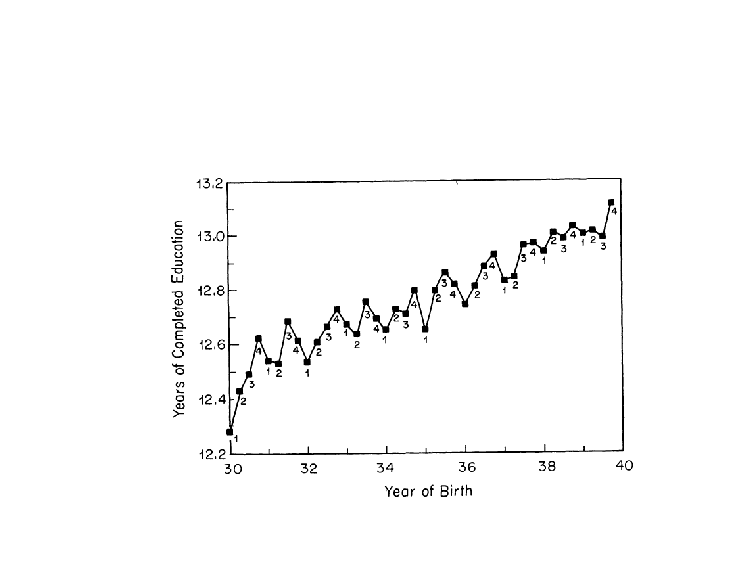
\includegraphics{./lecture_includes/qob_2.pdf}
	\end{figure}
	
\end{frame}

\begin{frame}{Forma reducida}
	
	¿Las diferencias en educación debido a diferentes trimestres de nacimiento se traducen en diferentes ingresos?
	
	\begin{figure}
	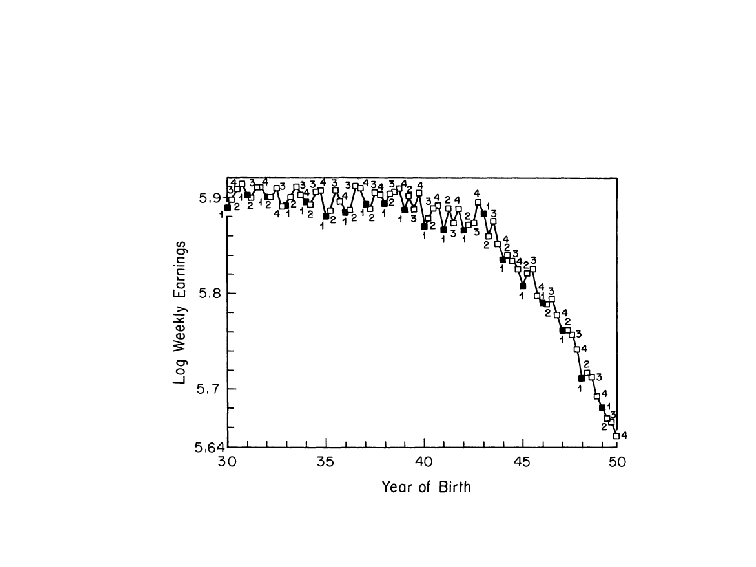
\includegraphics{./lecture_includes/qob_3.pdf}
	\end{figure}
	
\end{frame}

\begin{frame}{Modelo de Mínimos Cuadrados en Dos Etapas}
	
	\begin{itemize}
	\item El modelo causal es $$Y_i = X \pi + \delta S_i + \varepsilon$$
	\item La regresión de la primera etapa es: $$S_i=X\pi_{10} + \pi_{11}Z_i + \eta_{1i}$$
	\item La regresión de la forma reducida es: $$Y_i=X\pi_{20} + \pi_{21}Z_i+\eta_{2i}$$
	\item El análogo de muestra del estimador de Wald que ajusta por covariables: $\frac{\pi_{21}}{\pi_{11}}$
	\end{itemize}

\end{frame}

\begin{frame}{Mínimos Cuadrados en Dos Etapas}
	
	\begin{itemize}
	\item Angrist y Krueger instrumentan la educación utilizando tres variables ficticias para trimestre de nacimiento: una variable ficticia para el primer, segundo y tercer trimestre.
	\item Su regresión inicial de primera etapa es: $$S_i=X\pi_{10} + Z_{1i}\pi_{11} + Z_{2i}\pi_{12} + Z_{3i}\pi_{13}+\eta_1$$
	\item La segunda etapa es la misma que antes (incluyendo todos los controles $X$), pero los valores ajustados son de la nueva primera etapa $$Y_i = X \pi + \delta \widehat{S_i} + \epsilon$$
	\end{itemize}

\end{frame}

\begin{frame}{Resultados de la regresión de la primera etapa}

	El trimestre de nacimiento es un fuerte predictor del total de años de educación.
	
	\begin{figure}
	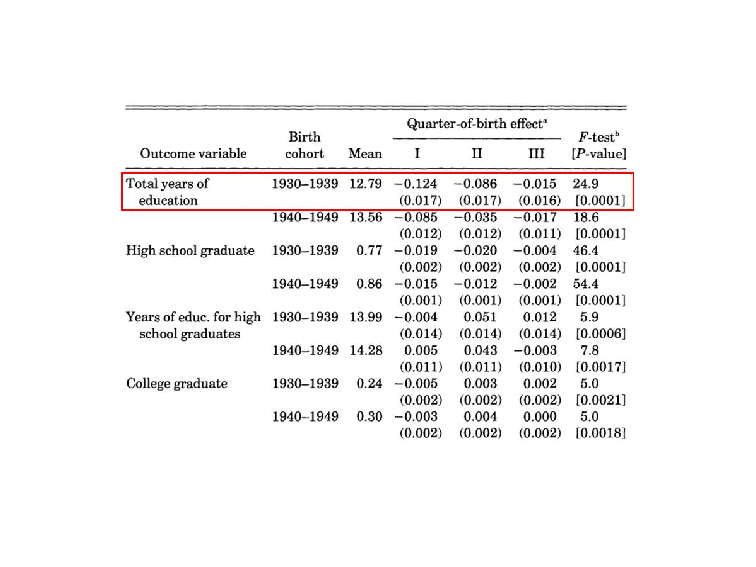
\includegraphics{./lecture_includes/qob_5.pdf}
	\end{figure}

\end{frame}

\begin{frame}{Estimaciones IV Cohortes de Nacimiento 20-29, Censo de 1980}
	
	\begin{figure}
	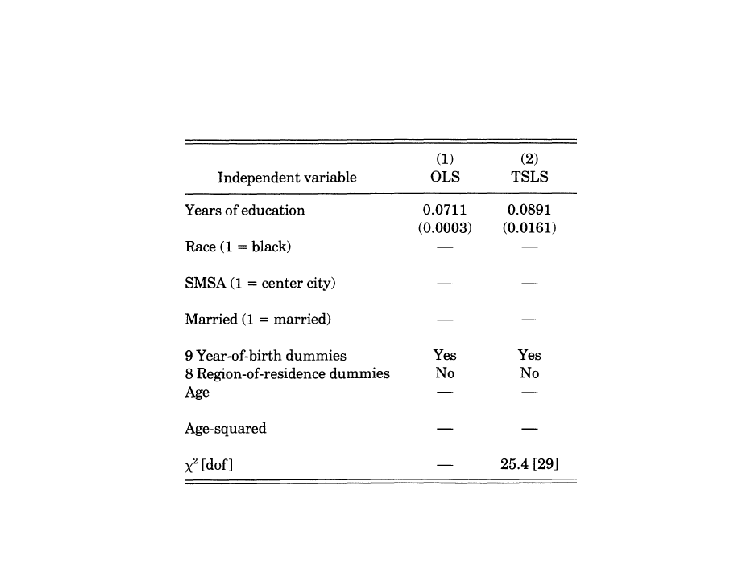
\includegraphics{./lecture_includes/qob_7.pdf}
	\end{figure}
	
\end{frame}




% \begin{frame}{180 instrumentos}

% \begin{itemize}
% \item Para mejorar la precisión en su modelo de mínimos cuadrados en dos etapas, incluyen más instrumentos (lo que causa una reducción del 40 por ciento en los errores estándar en 2SLS).
% \item Más instrumentos pueden aumentar la variación en la variable de educación predicha, reduciendo los errores estándar y estrechando los intervalos de confianza.
% \item Tres variables ficticias de trimestre de nacimiento interaccionadas con 50 variables ficticias de estado de nacimiento más 3 variables ficticias de trimestre de nacimiento interaccionadas con 9 variables ficticias de año de nacimiento (180 instrumentos).
% \item Incluye 50 variables ficticias de estado de nacimiento, por lo que la variabilidad en la educación en 2SLS se debe únicamente a diferencias en las estaciones de nacimiento, y esto se permite variar por estado y año de nacimiento por primera vez.
% \end{itemize}

% \end{frame}

% \begin{frame}{Más instrumentos}

% 	\begin{figure}
% 	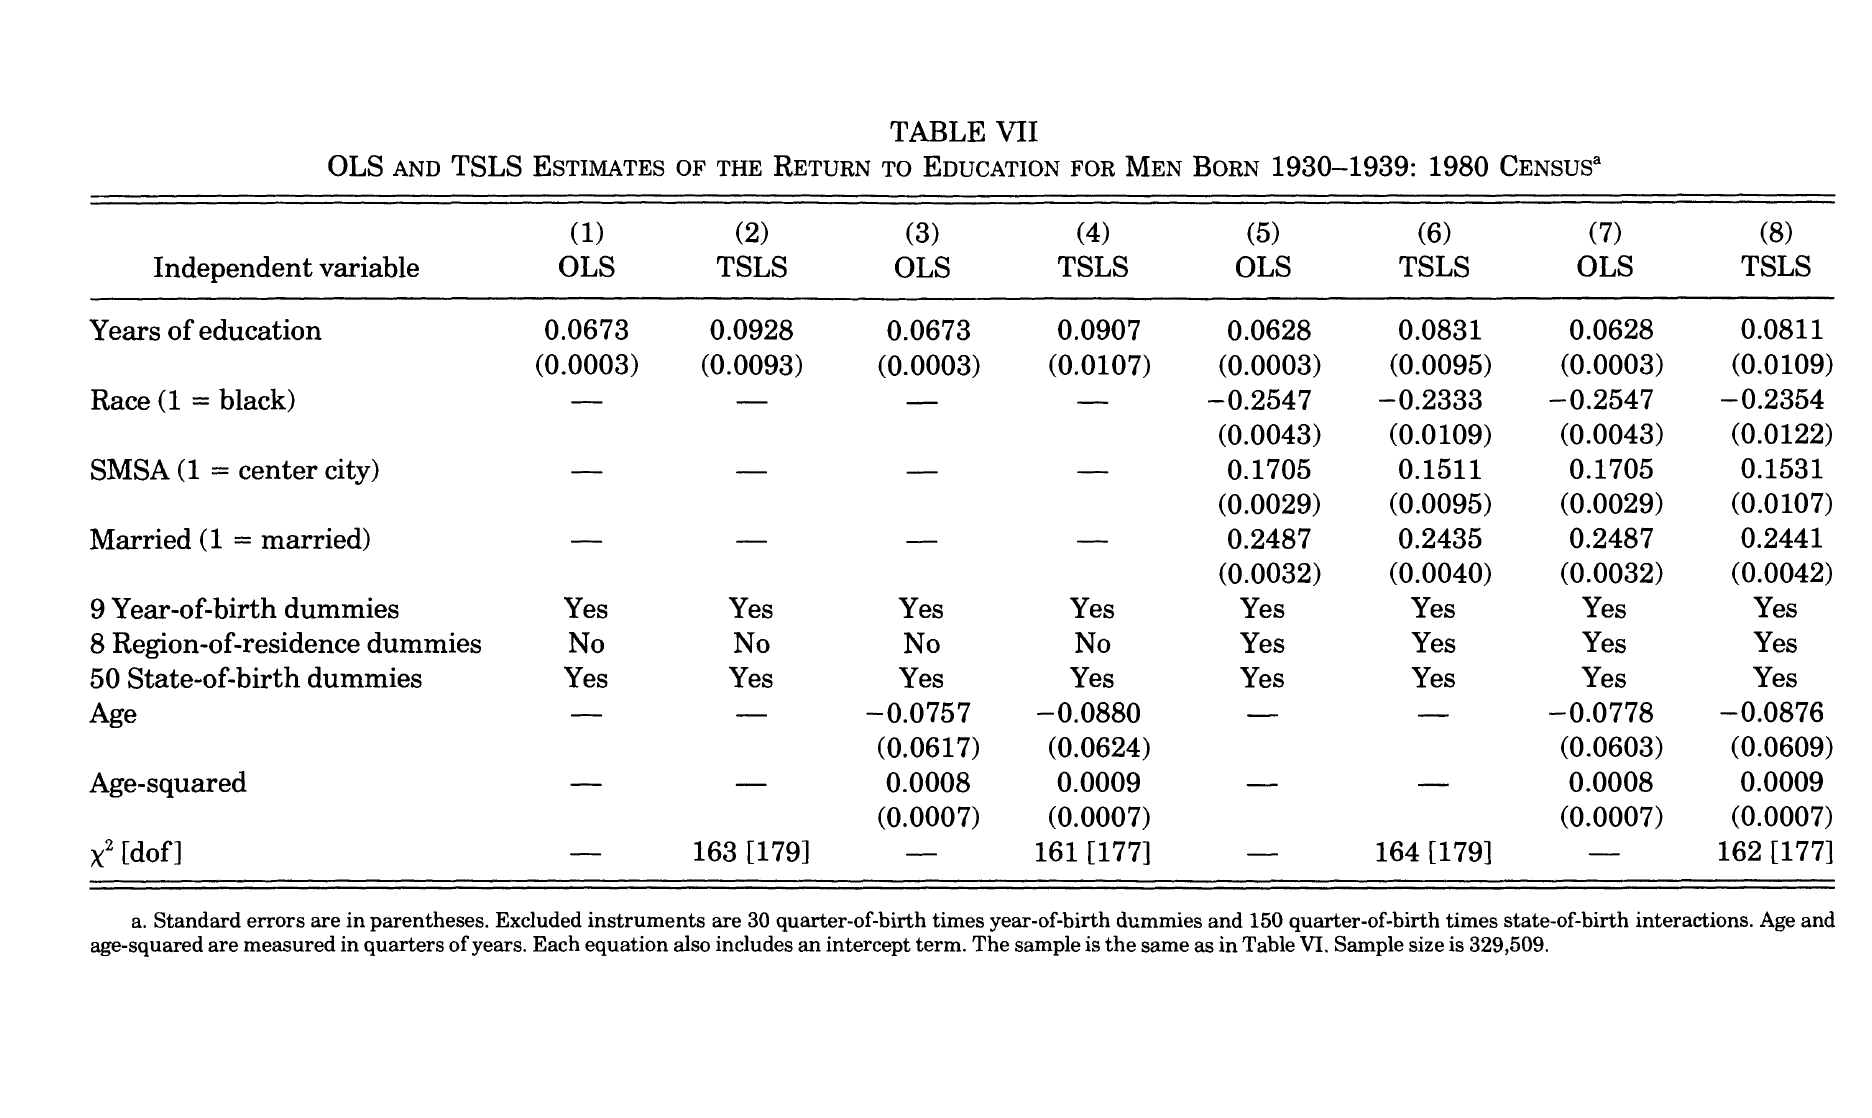
\includegraphics[scale=.18]{./lecture_includes/weak_qob3.png}
% 	\end{figure}
	
% \end{frame}



\subsection{Instrumentos débiles}

\begin{frame}{Instrumentos débiles}

\begin{quote}
``En la regresión por variables instrumentales, los instrumentos se denominan débiles si su correlación con los regresores endógenos, condicionada a cualquier control, está cerca de cero.'' -- Andrews, Stock y Sun (2018)
\end{quote}

\end{frame}

\begin{frame}{Instrumentos débiles}

\begin{itemize}
\item Mientras que la restricción de exclusión no es verificable, la primera etapa no es cero.
\item Los instrumentos débiles pueden ocurrir si las dos variables son independientes o si la muestra es pequeña.
\item Si tienes un instrumento débil, entonces el sesgo de 2SLS se centra en el sesgo de OLS y la solución termina siendo peor que la enfermedad.
\end{itemize}

\end{frame}

\begin{frame}{Instrumentos débiles}
	
	\begin{itemize}
	\item Un artículo importante sugiere que OLS y 2SLS son bastante similares, además de introducir la noción moderna de buscar ``instrumentos plausiblemente exógenos''.
	\item Pero a principios de los años 90, varios artículos mostraron que IV puede estar \emph{severamente} sesgado con instrumentos débiles y muchos instrumentos para una variable endógena.
	\item En el peor de los casos, si los instrumentos son tan débiles que no hay una primera etapa, entonces la distribución de muestreo de 2SLS se centra en el límite de probabilidad de OLS.
	\end{itemize}
\end{frame}

% \begin{frame}{Matrices e instrumentos}

% \begin{itemize}
% 	\item El modelo causal de interés es: $$Y=\beta X + \nu$$
% 	\item La matriz de variables instrumentales es Z con la ecuación de la primera etapa: $$X = {Z'}\pi + \eta$$
% \end{itemize}

% \end{frame}

% \begin{frame}{Instrumentos débiles y sesgo hacia OLS}

% \begin{itemize}
% 	\item Si $\nu_i$ del modelo causal y $\eta_i$ del modelo de primera etapa están correlacionados, entonces el estimador OLS $\widehat{\beta}_{OLS}$ en el modelo causal está sesgado.
% 	\item Para mostrar el sesgo de OLS, toma la diferencia media poblacional en $\beta$ menos el estimador $\beta_{OLS}$: $$E[\widehat{\beta}_{OLS} - \beta] = \frac{ Cov(\nu, X)}{Var(X)} = \frac{\sigma_{\nu \eta}}{\sigma^2_\eta}$$
% 	\item Nuestra esperanza es que con 2SLS, podamos llevar este sesgo a cero en la muestra finita y tener una estimación razonablemente no sesgada de $\beta$. 
% \end{itemize}

% \end{frame}

% \begin{frame}{Instrumentos débiles y sesgo de 2SLS hacia OLS}
	
% 	\begin{itemize}
% 	\item Los instrumentos fuertes reducen el término de sesgo, $\frac{\sigma_{\nu \eta}}{\sigma^2_\eta}$, a un valor escalado inconsecuente (pero no pueden llegar a cero).
% 	\item Podemos derivar el sesgo aproximado de 2SLS como: $$E[\widehat{\beta}_{2SLS} - \beta] \approx \frac{\sigma_{\nu \eta}}{\sigma^2_\eta} \frac{1}{F+1}$$
% 	\item Considera la intuición que todo ese trabajo nos proporcionó ahora: si la primera etapa es débil (es decir, $F\rightarrow{0}$), entonces el sesgo de 2SLS se aproxima a $\frac{\sigma_{\nu \eta}}{\sigma^2_\eta}$.
% 	\end{itemize}
% \end{frame}

% \begin{frame}{Instrumentos débiles y sesgo hacia OLS}

% \begin{itemize}
% 	\item Esto es lo mismo que el sesgo de OLS cuando $\pi=0$ en la segunda ecuación de la diapositiva anterior (es decir, no hay relación en la primera etapa) $\sigma^2_x = \sigma^2_\eta$ y, por lo tanto, el sesgo de OLS $\frac{\sigma_{\nu \eta}}{\sigma^2_\eta}$ se convierte en $\frac{\sigma_{\nu \eta}}{\sigma^2_\eta}$.
% 	\item Pero si la primera etapa es muy fuerte ($F\rightarrow{\infty}$), entonces el sesgo de 2SLS se aproxima a 0.
% 	\item Lo interesante es que puedes probar esto con una prueba F sobre la significación conjunta de $Z$ en la primera etapa.
% 	\item Por lo tanto, es absolutamente crítico que elijas instrumentos que estén fuertemente correlacionados con el regresor endógeno; de lo contrario, la cura es peor que la enfermedad.
% \end{itemize}

% \end{frame}


% \begin{frame}{Instrumentos débiles - Añadiendo más instrumentos}
	
% 	\begin{itemize}
% 	\item Añadir más instrumentos débiles aumentará el sesgo de 2SLS
% 		\begin{itemize}
% 		\item Al agregar más instrumentos sin poder predictivo, el estadístico $F$ de la primera etapa tiende a cero y el sesgo aumenta
% 		\item Veremos esto más de cerca cuando cubramos el diseño de indulgencia
% 		\end{itemize}
% 	\item Si el modelo está ``exactamente identificado'' -- es decir, el mismo número de variables instrumentales que covariables endógenas -- el sesgo de instrumentos débiles es menos problemático
% 	\end{itemize}
% \end{frame}

% \begin{frame}{Problema de instrumentos débiles}

% \begin{itemize}
% 	\item Después del estudio de Angrist y Krueger, surgieron nuevos artículos que destacan problemas relacionados con instrumentos débiles y sesgo en muestras finitas
% 	\item Los artículos clave son Nelson y Startz (1990), Buse (1992), Bekker (1994) y especialmente Bound, Jaeger y Baker (1995)
% 	\item Bound, Jaeger y Baker (1995) destacaron este problema para el estudio de Angrist y Krueger.  
% \end{itemize}

% \end{frame}

% \begin{frame}{Bound, Jaeger y Baker (1995)}

% Recuerda que AK presentan hallazgos de la expansión de sus instrumentos para incluir muchas interacciones (es decir, modelo saturado)
% 		\begin{enumerate}
% 		\item Variables ficticias de trimestre de nacimiento $\rightarrow$ 3 instrumentos
% 		\item Variables ficticias de trimestre de nacimiento $+$ (trimestre de nacimiento) $\times$ (año de nacimiento) $+$ (trimestre de nacimiento) $\times$ (estado de nacimiento) $\rightarrow$ 180 instrumentos
% 		\end{enumerate}
% Así que si alguno de estos es débil, entonces el sesgo aproximado de 2SLS empeora.

% \end{frame}

% \begin{frame}{Añadiendo instrumentos en Angrist y Krueger}
	
% 	\begin{figure}
% 	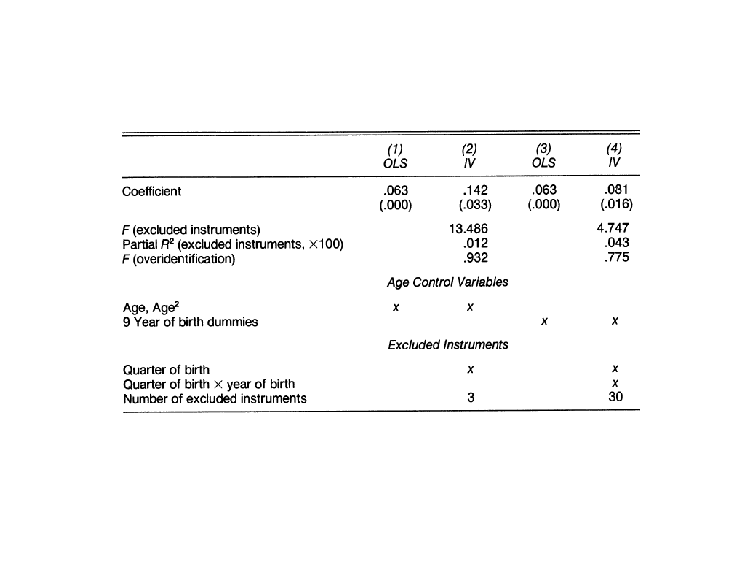
\includegraphics{./lecture_includes/ak_iv1.pdf}
% 	\end{figure}
	
% Añadir más instrumentos débiles reduce el estadístico $F$ de la primera etapa y aumenta el sesgo de 2SLS. Observa que también se ha acercado a OLS. 
	
% \end{frame}

% \begin{frame}{Añadiendo instrumentos en Angrist y Krueger}
	
% 	\begin{figure}
% 	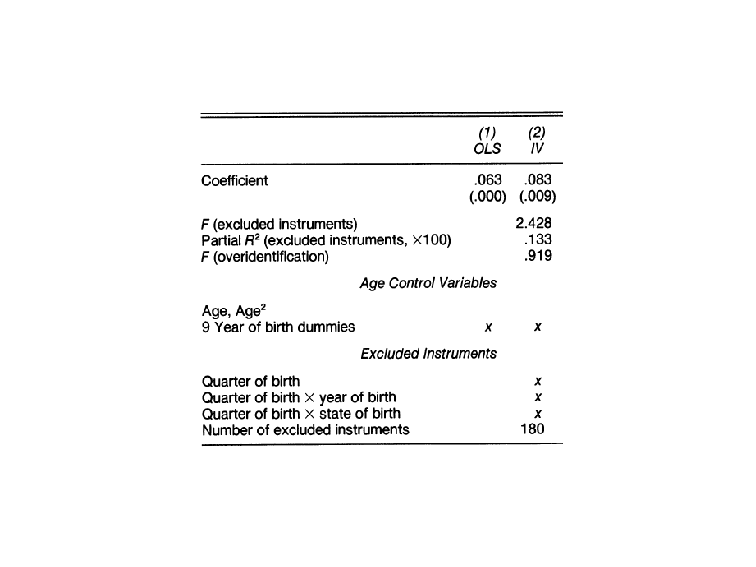
\includegraphics{./lecture_includes/ak_iv2.pdf}
% 	\end{figure}
	
% Más instrumentos aumentan la precisión, pero disminuyen $F$, por lo tanto, sabemos que el problema ha empeorado.
	
% \end{frame}





% \begin{frame}{Consejos IV: Instrumentos débiles}

% 	\begin{itemize}
% 	\item Excelente revisión de Keane y Neal (2021) ``Una Guía Práctica para Instrumentos Débiles'', así como de Andrews, Stock y Sun (2018)
% 	\item Stock, Wright y Yogo (2002) encontraron que los estadísticos $F$ sobre la excluibilidad del instrumento de la primera etapa mayores a 10 funcionaron bien en Monte Carlos con homocedasticidad, pero 2SLS tiene propiedades deficientes aquí
% 		\begin{itemize}
% 		\item Bajo poder
% 		\item Errores estándar artificialmente bajos cuando la endogeneidad es severa
% 		\item Esto causa que las pruebas $t$ sean engañosas
% 		\end{itemize}
% 	\end{itemize}

% \end{frame}

% \begin{frame}{Consejos IV: Instrumentos débiles}

% \begin{quote}
% ``En el caso principal con un solo regresor endógeno, recomendamos que los investigadores juzguen la fuerza del instrumento basado en el estadístico $F$ efectivo de Montiel Olea y Pflueger (2013). Si hay un solo instrumento, recomendamos informar intervalos de confianza robustos de Anderson-Rubin. Estos son efectivos independientemente de la fuerza de los instrumentos, y por lo tanto deberían ser informados sin importar el valor del $F$ de la primera etapa. Finalmente, si hay múltiples instrumentos, la literatura aún no ha convergido en un procedimiento único, pero recomendamos elegir entre los varios procedimientos robustos disponibles que son eficientes cuando los instrumentos son fuertes.'' -- Andrews, Stock y Sun (2018)
% \end{quote}

% \end{frame}


% \begin{frame}{Consejos IV: Instrumentos débiles}

% \begin{itemize}
% 	\item Anderson-Rubin alivia en gran medida este problema y debería ser utilizado incluso con instrumentos muy fuertes siempre que el $F$ de la primera etapa esté bien por encima de 10 (Lee, et al. 2020 dice 104.7)
% 	\item Se recomiendan umbrales más altos, y aun así se sugieren pruebas robustas a menos que el $F$ esté en los miles
% 	\item Keane y Neal (2021) escriben: ``para evitar rechazar en exceso la nulidad cuando $\beta_{2SLS}$ se desplaza en la dirección del sesgo de OLS, uno debería confiar en la prueba de Anderson-Rubin en lugar de la prueba $t$ incluso cuando el estadístico $F$ de la primera etapa esté en los miles.'' 
% \end{itemize}

% \end{frame}

% \begin{frame}{DGP heterocedástico}

% \begin{itemize}
% \item Evaluar los estadísticos $F$ aceptables de la primera etapa significa, en la práctica, considerar el impacto de la heterocedasticidad
% \item Con múltiples instrumentos, es inapropiado usar un $F$ convencional o robusto a la heterocedasticidad para evaluar la fuerza del instrumento
% \item Andrews, et al. (2019) sugieren el estadístico $F$ efectivo de primera etapa de Olea y Pflueger (2013)
% \item El caso de identificación justa con un solo instrumento se reduce al $F$ robusto convencional y al Wald de Kleibergen y Paap (2006)
% \end{itemize}

% \end{frame}



\end{document}




\subsection{Local average treatment effects}

\begin{frame}{Constant vs heterogenous treatment effects}

\begin{itemize}
\item IV was modeled using realized outcomes, which clouded causal inference
\item But also tended to assume constant treatment effects
\item When you introduced heterogenous treatment effects, IV became more complex 
\end{itemize}

\end{frame}

\begin{frame}{Some background}

\begin{itemize}
\item October 2021's Nobel Prize in economics went to Card, Angrist and Imbens (the last two for work 1990s work on IV)
\item Angrist writes a dissertation using randomized instruments (Vietnam draft), goes to Harvard, overlaps with Imbens for a year, they are mentored by Gary Chamberlain, work with Don Rubin, write their famous LATE paper
\item Chamberlain recommends modifying Rubin's potential outcomes framework (instead of their original latent index modeling) and that seems to make the work more generally attractive (outside economics)
\item Let's spend twenty minutes listening to them
\end{itemize}

\end{frame}

\begin{frame}{Angrist, Imbens and Harvard}


Josh Angrist on the negative results at the time (10 min)

\url{https://youtu.be/ApNtXe-JDfA?t=1885}

Guido Imbens on the reception of their work (10 min)

\url{https://youtu.be/cm8V65AS5iU?t=799}

\end{frame}




\begin{frame}{Potential treatment concept}
	
``Potential treatment status'' ($D^j$) is like potential outcomes the thought experiment; it's not the observed treatment status $D$ until we switch between them with the instrument's assignment
\bigskip
		\begin{itemize}
		\item $D^1_{i} = i$'s treatment status when $Z_i=1$
		\item $D^0_{i} = i$'s treatment status when $Z_i=0$
		\end{itemize}
\bigskip
We'll represent outcomes as a function of both treatment status and instrument status. In other words, $Y_i(D_i=0,Z_i=1)$ is represented as $Y_i(0,1)$

\end{frame}




\begin{frame}{Identification}
		
	\begin{enumerate}
	\item Stable Unit Treatment Value Assumption (SUTVA)
	\item Random Assignment
	\item Exclusion Restriction
	\item Nonzero First Stage
	\item Monotonicity
	\end{enumerate}
\end{frame}


\begin{frame}{SUTVA}

\begin{block}{SUTVA with respect to IV}
In the IV context, SUTVA means the \textbf{potential treatments} for any unit do not (1) vary with the instruments assigned to other units, and for each unit, (2) there are no different forms of versions of each instrument level, which lead to different potential treatments
\end{block}

\bigskip

Once you make $D^1_i$, $D^0_i$ based on a scalar, you've invoked SUTVA because this means your potential outcome is not based on other's assignment and it means there's no hidden variation in the instrument

\bigskip

Example:   The instrument is a randomly generated draft number. When your friend, $i'$, gets drafted, you, $i$, somehow get drafted too even though you didn't get assigned with your draft number


\end{frame}

		


\begin{frame}{Independence assumption}
	
	\begin{block}{Independence assumption}
	$\{Y_i(D^1_i,1),Y_i(D^0_i,0),D^1_{i},D^{0}_i\} \independent{Z}_i$
	\end{block}

\begin{itemize}	
\item Instruments are assigned independent of potential treatment status and potential outcomes
\item Independence is ensured by physical randomization, but perhaps other assignments could too (e.g., alphabetized assignment)
\item Example: Random draft numbers generated by a random number generator
\end{itemize}

\end{frame}


\begin{frame}{Independence}

		 \textbf{Implications of independence}: First stage measures the causal effect of $Z_i$ on $D_i$:
			\begin{eqnarray*}
			E[D_i|Z_i=1] - E[D_i|Z_i=0] &=& E[D^1_{i} | Z_i = 1] - E[D^0_{i}|Z_i = 0] \\
			&=& E[D^1_{i} - D^0_{i}]
			\end{eqnarray*}

\end{frame}

\begin{frame}{Independence}

			 \textbf{Implications of independence}: Reduced form measures the causal effect of $Z_i$ on $Y_i$
			\begin{eqnarray*}
			E[Y_i | Z_i=1] - E[Y_i | Z_i=0] &=& E[Y_i(D^1_{i},1)|Z_i = 1] \\
			&& - E[Y_i(D^0_{i},0) | Z_i = 0] \\
			&=&E[Y_i(D^1_{i},1)] - E[Y_i(D^0_{i},0)]
			\end{eqnarray*}
			
			\bigskip
			
			But independence is not enough to for this to mean we've identified the causal effect of $D$ on $Z$ as $Z$ could be operating directly not ``only through'' the treatment -- for that we need exclusion
\end{frame}

\begin{frame}[plain]
\frametitle{Exclusion Restriction}

	\begin{block}{Exclusion Restriction}
	$\textbf{Y(D,Z)}=\textbf{Y(D,Z')}$ for all $\textbf{Z}$, $\textbf{Z'}$, and for all $\textbf{D}$
	\end{block}
	
\begin{itemize}
\item Notice how in the notation, $Z$ is changing to $Z'$, but $D$ is held fixed and as a result of it being held fixed, $Y$ does not change?
\item  That's the ``only through'' part. Any effect of $Z$ on $Y$ must be via the effect of $Z$ on $D$.
\item Recall the DAG and the \emph{missing arrows} from $Z$ to $\nu$ and from $Z$ to $Y$ directly
\item \textbf{Violation example}:  Your draft number causes you to go to graduate school to avoid the draft, but graduate school changes your wages, therefore exclusion is violated even though instrument was random
\end{itemize}
	
\end{frame}





\begin{frame}{Exclusion restriction}
	
	\begin{itemize}
	\item Use the exclusion restriction to define potential outcomes indexed solely against treatment status (regardless of instrument assignment): 
		\begin{eqnarray*}
		 Y^1_{i} &=& Y_i(1,1) = Y_i(1,0) \\
		 Y^0_{i} &=& Y_i(0,1) = Y_i(0,0)
		\end{eqnarray*}
	\item Rewrite switching equation:
		\begin{eqnarray*}
		Y_i &=& Y_i(0,Z_i) + [Y_i(1,Z_i) - Y_i(0,Z_i)]D_i \\
		Y_i &=& Y^0_{i} + [Y^1_{i} - Y^0_{i}]D_i \\
		Y_i &=& Y^0_i + \delta_iD_i
		\end{eqnarray*}
	\item Notice here that $D_i$ will only change if the instrument assignment causes it to change, and thus the average causal effect picked up will only be for those who reply to their instrument assignment
	\end{itemize}

\end{frame}

\begin{frame}{Know your treatment and instrument assignment mechanism}

People tend to target exclusion arguments when they see them, because except under very special situations like homogenous treatment effects with overidentification, they're based on untestable assumptions

\bigskip

Angrist and Krueger (2001) note ``In our view, good instruments often come from detailed knowledge of the economic mechanism and institutions determining the regressor of interest.''  

\bigskip

You simply can't avoid the importance of deep knowledge of treatment and instrument assignment, as those are literally in the identifying assumptions (e.g., independence, exclusion)

\end{frame}


\begin{frame}{Strong first stage}
	
	\begin{block}{Nonzero Average Causal Effect of $Z$ on $D$}
	$E[D^1_{i} - D^0_{i}]\neq{0}$
	\end{block}
				
\begin{itemize}
\item Recall the weak instrument literature from earlier (AR, $F$ very large)
\item $D^1$ means instrument is turned on, and $D^0$ means it is turned off. We need treatment to change when instrument changes.
\item $Z$ has to have some statistically significant effect on the average probability of treatment
\item Example: Check whether a high draft number makes you more likely to get drafted and vice versa
\item Finally -- a testable assumption. We have data on $Z$ and $D$
\end{itemize}

\end{frame}			


\begin{frame}{Monotonicity}
	
	\begin{block}{Monotonicity}
	Either $\pi_{1i}\geq{0}$ for all $i$ or $\pi_{1i}\leq{0}$ for all $i=1, \dots, N$
	\end{block}

\begin{itemize}

\item Recall that $\pi_{1i}$ is the reduced form causal effect of the instrumental variable on an individual $i$'s treatment status.  
\item Monotonicity requires that the instrumental variable (weakly) operate in the same direction on all individual units.  
\item ``changing the instrument's value does not induce two-way flows in and out treatment'' -- Michal Kolesar (2013)
\item Anyone affected by the instrument is affected \emph{in the same direction} (i.e., positively or negatively, but not both).
\item \textbf{Example of a violation}: People with high draft number dodge the draft but would have volunteered had they gotten a low number

\end{itemize}

\end{frame}


\begin{frame}{Local average treatment effect}

	If all 1-5 assumptions are satisfied, then IV estimates the \textbf{local average treatment effect (LATE)} of $D$ on $Y$: $$\delta_{IV,LATE} =\frac{\text{Effect of Z on Y}}{\text{Effect of Z on D}}$$

\end{frame}	

\begin{frame}{Estimand}

	\vskip3pt plus.1fill
				
	Instrumental variables (IV) estimand: 
	\begin{align*}
	\delta_{IV,LATE} & = \frac{E[Y_i(D^1_i, 1) - Y_i(D^0_i, 0)]}{E[D^1_i - D^0_i]}& \\
	& = E[(Y^1_i - Y^0_i) | D^1_i - D^0_i = 1]
	\end{align*}

\end{frame}		

\begin{frame}{Local Average Treatment Effect}
	
	\begin{itemize}
	\item The LATE parameters is the average causal effect of $D$ on $Y$ for those whose treatment status was changed by the instrument, $Z$
	\item For example, IV estimates the average effect of military service on earnings for the subpopulation who enrolled in military service because of the draft but would not have served otherwise. 
	\item LATE does not tell us what the causal effect of military service was for patriots (volunteers) or those who were exempted from military service for medical reasons 
	\end{itemize}
	
\end{frame}


\begin{frame}{LATE and subpopulations}
	
IV estimates the average treatment effect for only one of these subpopulations:
		\begin{enumerate}
		\item \underline{Always takers}: My family have always served, so I serve regardless of whether I am drafted
		\item \underline{Never takers}: I'm a contentious objector so under no circumstances will I serve, even if drafted
		\item \underline{Defiers}: When I was drafted, I dodged. But had I not been drafted, I would have served. I am a man of contradictions.
		\item \textbf{Compliers}: I only enrolled in the military because I was drafted otherwise I wouldn't have served
		\end{enumerate}
\end{frame}


\begin{frame}[plain]
	\begin{columns}[t]
	\scriptsize
	\column{.4\textwidth}
	\begin{block}{Never-Takers}
		$D^1_i - D^0_i = 0$ \\
		$Y_i(0,1) - Y_i(0,0) = 0$ \\
		By \textcolor{red}{Exclusion Restriction}, causal effect of $Z$ on $Y$ is zero.
	\end{block}
	\begin{block}{Defier}
		$D^1_i - D^0_i = -1$ \\
		$Y_i(0,1) - Y_i(1,0) = Y_i(0) - Y_i(1)$ \\
		By \textcolor{red}{Monotonicity}, no one in this group
	\end{block}
	\column{.4\textwidth}
	\begin{block}{Complier}
		$D^1_i - D^0_i = 1$ \\
		$Y_i(1,1) - Y_i(0,0) = Y_i(1) - Y_i(0)$ \\
		Average Treatment Effect among Compliers
	\end{block}
	\begin{block}{Always-taker}
		$D^1_i - D^0_i = 0$ \\
		$Y_i(1,1) - Y_i(1,0) = 0$ \\
		By \textcolor{red}{Exclusion Restriction}, causal effect of $Z$ on $Y$ is zero.
	\end{block}
	\end{columns}
\end{frame}


\begin{frame}{Monotonicity Ensures that there are no defiers}
	
	\begin{itemize}
	\item Why is it important to not have defiers?
		\begin{itemize}
		\item If there were defiers, effects on compliers could be (partly) canceled out by opposite effects on defiers
		\item One could then observe a reduced form which is close to zero even though treatment effects are positive for everyone (but the compliers are pushed in one direction by the instrument and the defiers in the other direction)
		\end{itemize}
	\item Monotonicity assumes there are no defiers (there are weak and strong versions of it too)
	\end{itemize}

\end{frame}

\begin{frame}{LATE is not the ATE}
	
	\begin{itemize}
	\item IV estimates the average causal effect for those units affected by the instrument (i.e., complier causal effects)
	\item Work in the mid-2000s found that with continuous instruments, it could be possible to extrapolate from the LATE to the aggregate parameter (marginal treatment effect literature)
	\item I'll wait to discuss that literature but know it's coming and important to learn
	\end{itemize}

\end{frame}

		
\begin{frame}{Sensitivity to assumptions: exclusion restriction}
	
\begin{itemize}
	
\item Someone at risk of draft (low lottery number) changes education plans to retain draft deferments and avoid conscription. 

\item Increased bias to IV estimand through two channels:
		\begin{itemize}
		\item Average direct effect of $Z$ on $Y$ for compliers
		\item Average direct effect of $Z$ on $Y$ for noncompliers multiplied by odds of being a non-complier
		\end{itemize}

\item Severity depends on: 
		\begin{itemize}
		\item Odds of noncompliance (smaller $\rightarrow$ less bias)
		\item ``Strength'' of instrument (stronger $\rightarrow$ less bias)
		\item Effect of the alternative channel on $Y$
		\end{itemize}
\end{itemize}

\end{frame}


\begin{frame}{Sensitivity to assumptions: Monotonicity violations}

\begin{itemize}

\item Someone who would have volunteered for Army when not at risk of draft (high lottery number) chooses to avoid military service when at risk of being drafted (low lottery number)
	
\item Bias to IV estimand (multiplication of 2 terms):
		\begin{itemize}
		\item Proportion defiers relative to compliers
		\item Difference in average causal effects of $D$ on $Y$ for compliers and defiers
		\end{itemize}
\item Severity depends on:
		\begin{itemize}
		\item Proportion of defiers (small $\rightarrow$ less bias)
		\item ``Strength'' of instrument (stronger $\rightarrow$ less bias)
		\item Variation in effect of $D$ on $Y$ (less $\rightarrow$ less bias)
		\end{itemize}
\end{itemize}
		
\end{frame}

	
		

\section{Application}

\subsection{Data visualization and necessary evidence}

\begin{frame}{Practical advice}

\begin{itemize}
\item Before we move into applications, let's talk about pictures
\item It's very easy for causal inference to become a black box, but the more it's a black box, the less people will believe your analysis 
\item There's also recent evidence that IV papers show signs of publication bias with a large spike in $p$-values at 0.05 (unlike RCT and RDD)
\item Pictures are crucial, but it's particular kinds of pictures you need to show for IV that I want to emphasize (not just any data visual)

\end{itemize}

\end{frame}



\begin{frame}{Show Wald Quantities}

Present your main results as Wald quantites in beautiful pictures of simple correlations even if you're estimating with 2SLS
	\begin{itemize}
	\item Show pictures of the \textcolor{blue}{first stage}. If you can't see the correlation in the first stage, you have a weak instrument problem
	\item Show instead pictures of the \textcolor{blue}{reduced form}.  If you can't see the correlation in the reduced form, it's likely not there.
	\end{itemize}
	
	\bigskip
	
This can be challenging as not every IV design will lend itself to easy pictures though which is why it helps if you can familiarize yourself with a range of pictures for inspiration	

\end{frame}



\begin{frame}{IV advice: Picturing my instrument}
	
	\begin{figure}
	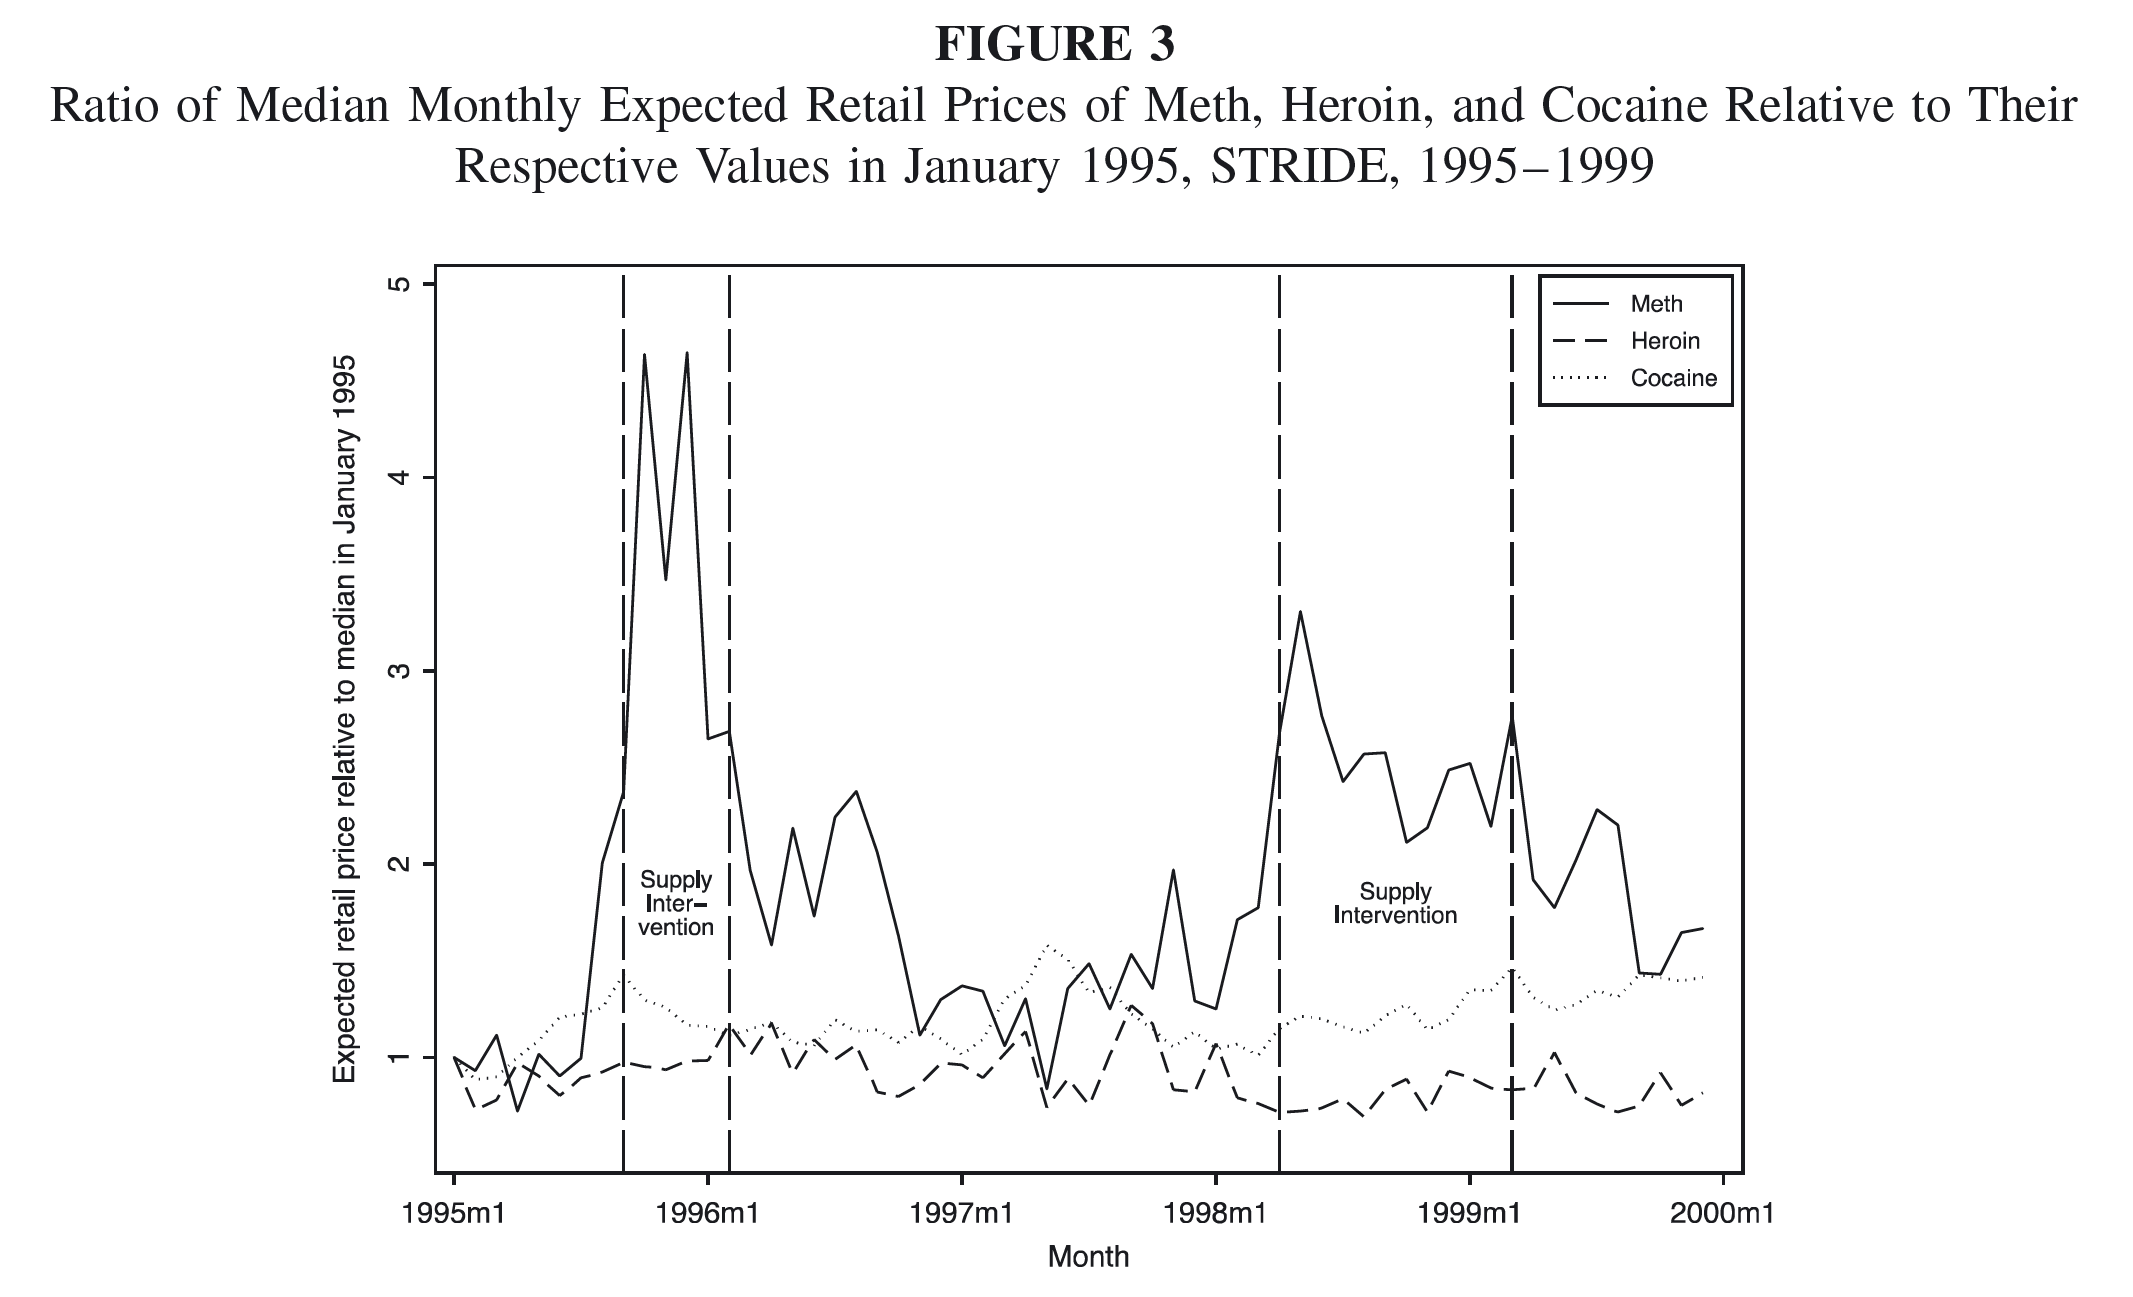
\includegraphics[scale=0.15]{./lecture_includes/keith_1.png}
	\end{figure}
	
\end{frame}


\begin{frame}{IV advice: Picturing the first stage}
	
	\begin{figure}
	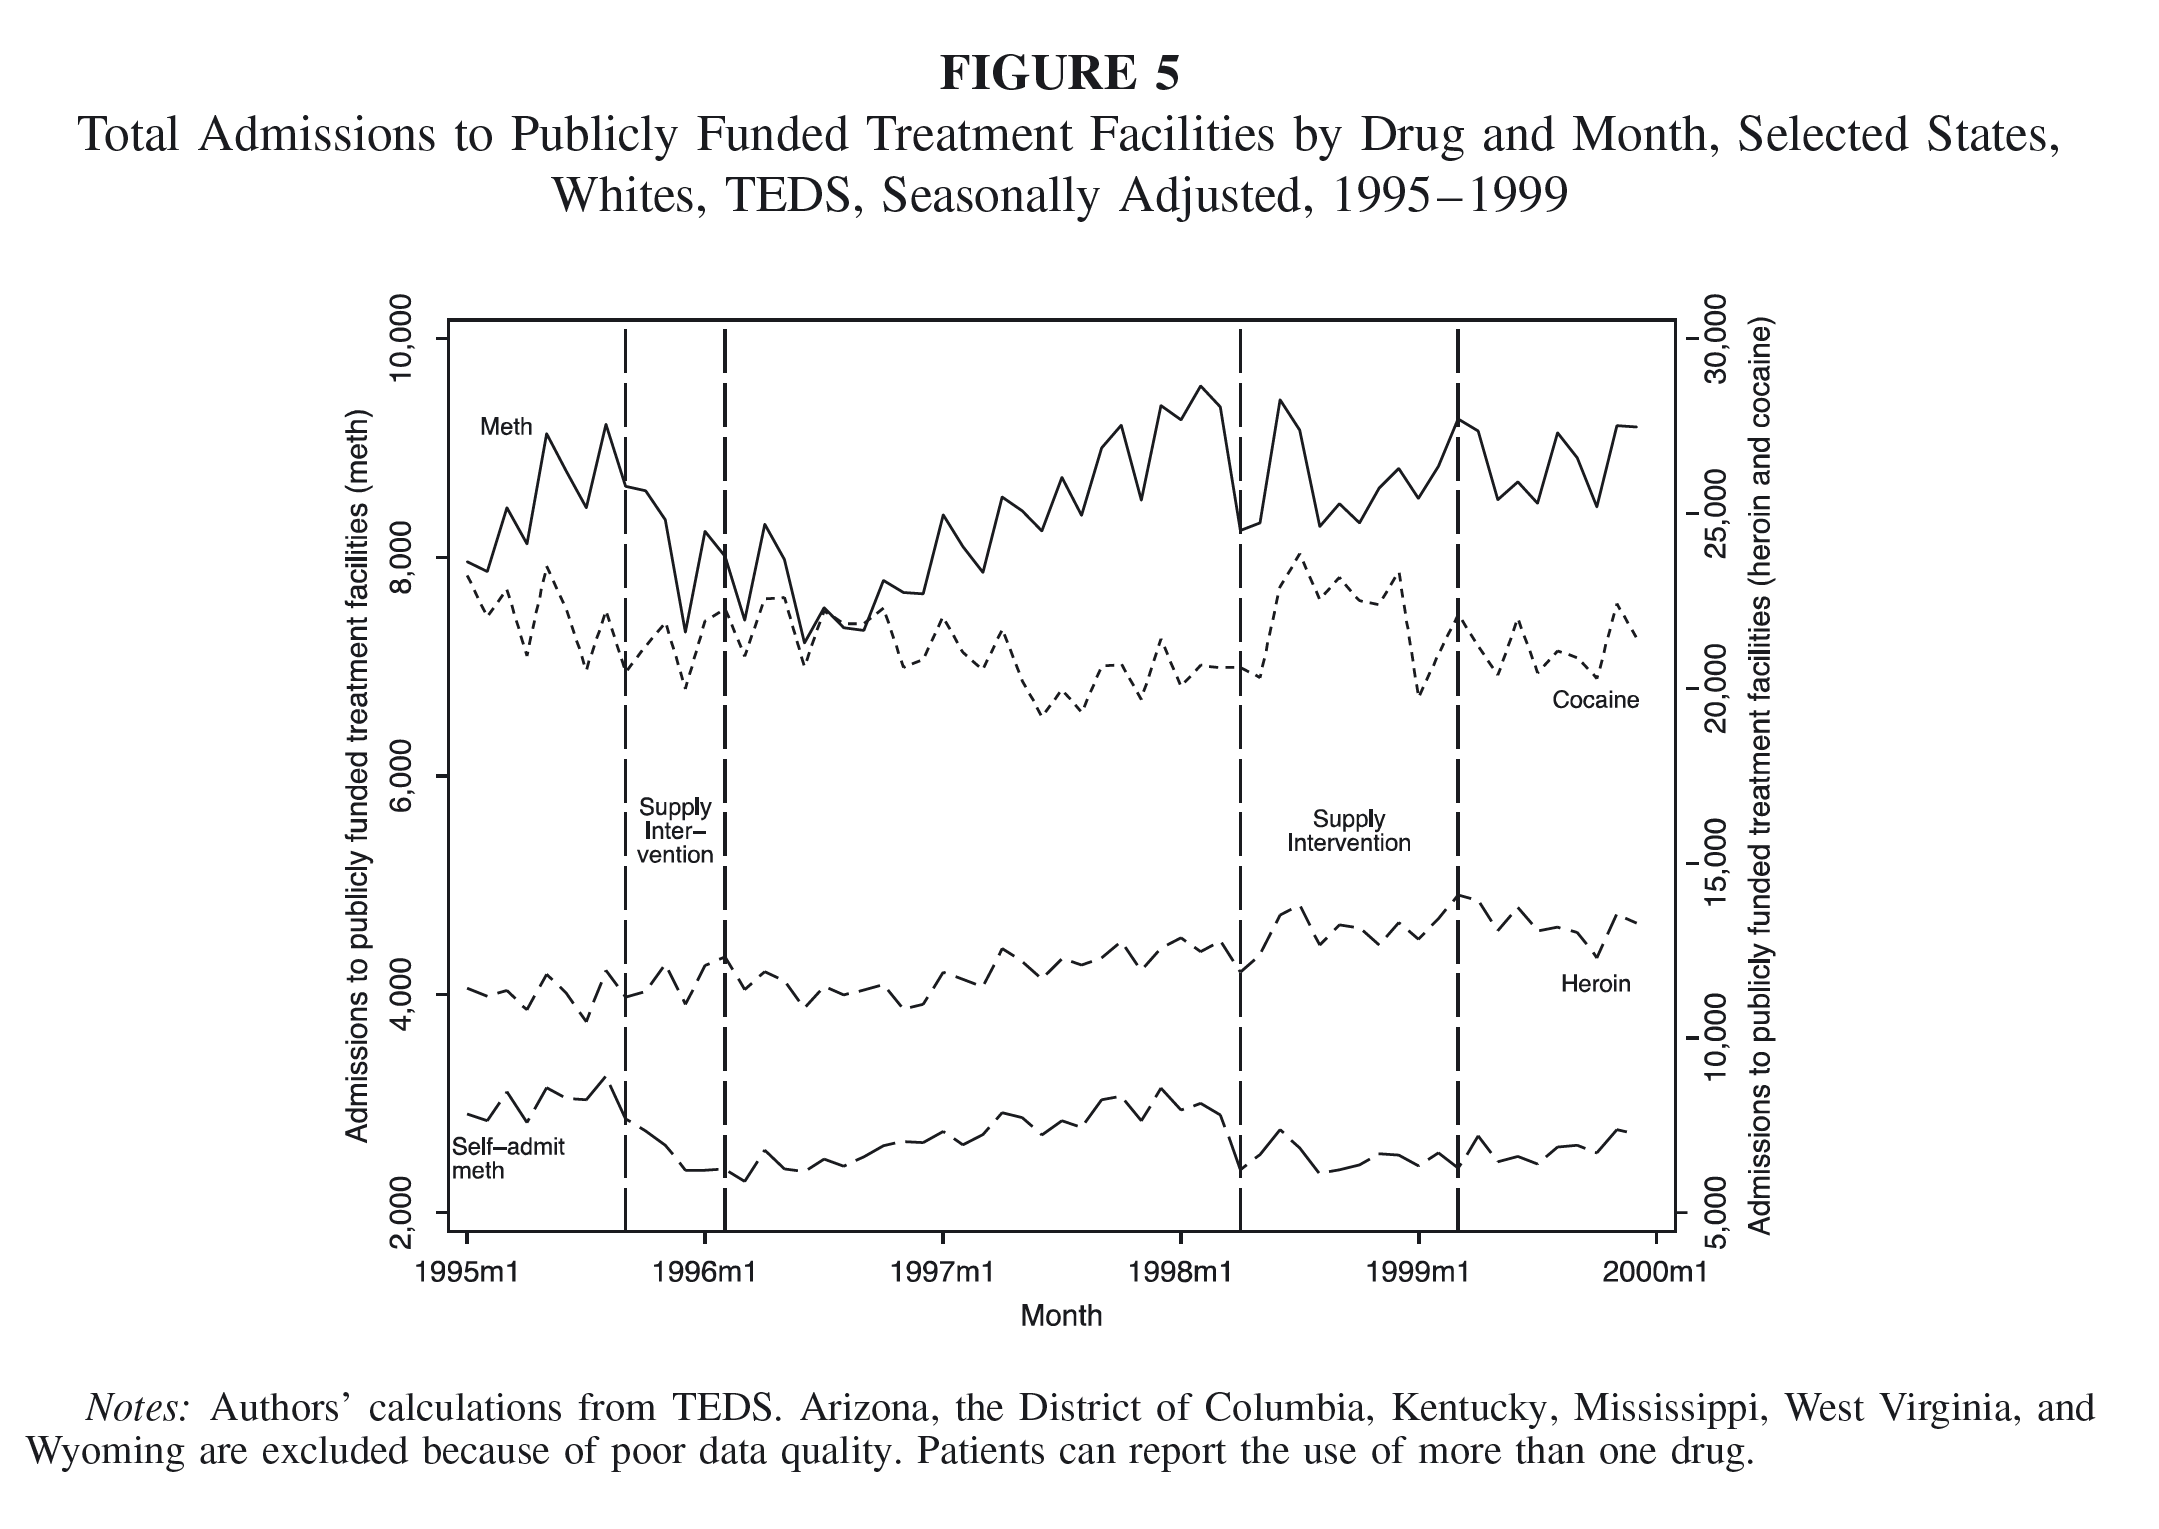
\includegraphics[scale=0.15]{./lecture_includes/keith_3.png}
	\end{figure}
	
\end{frame}

\begin{frame}{IV advice: Picturing the reduced form}
	
	\begin{figure}
	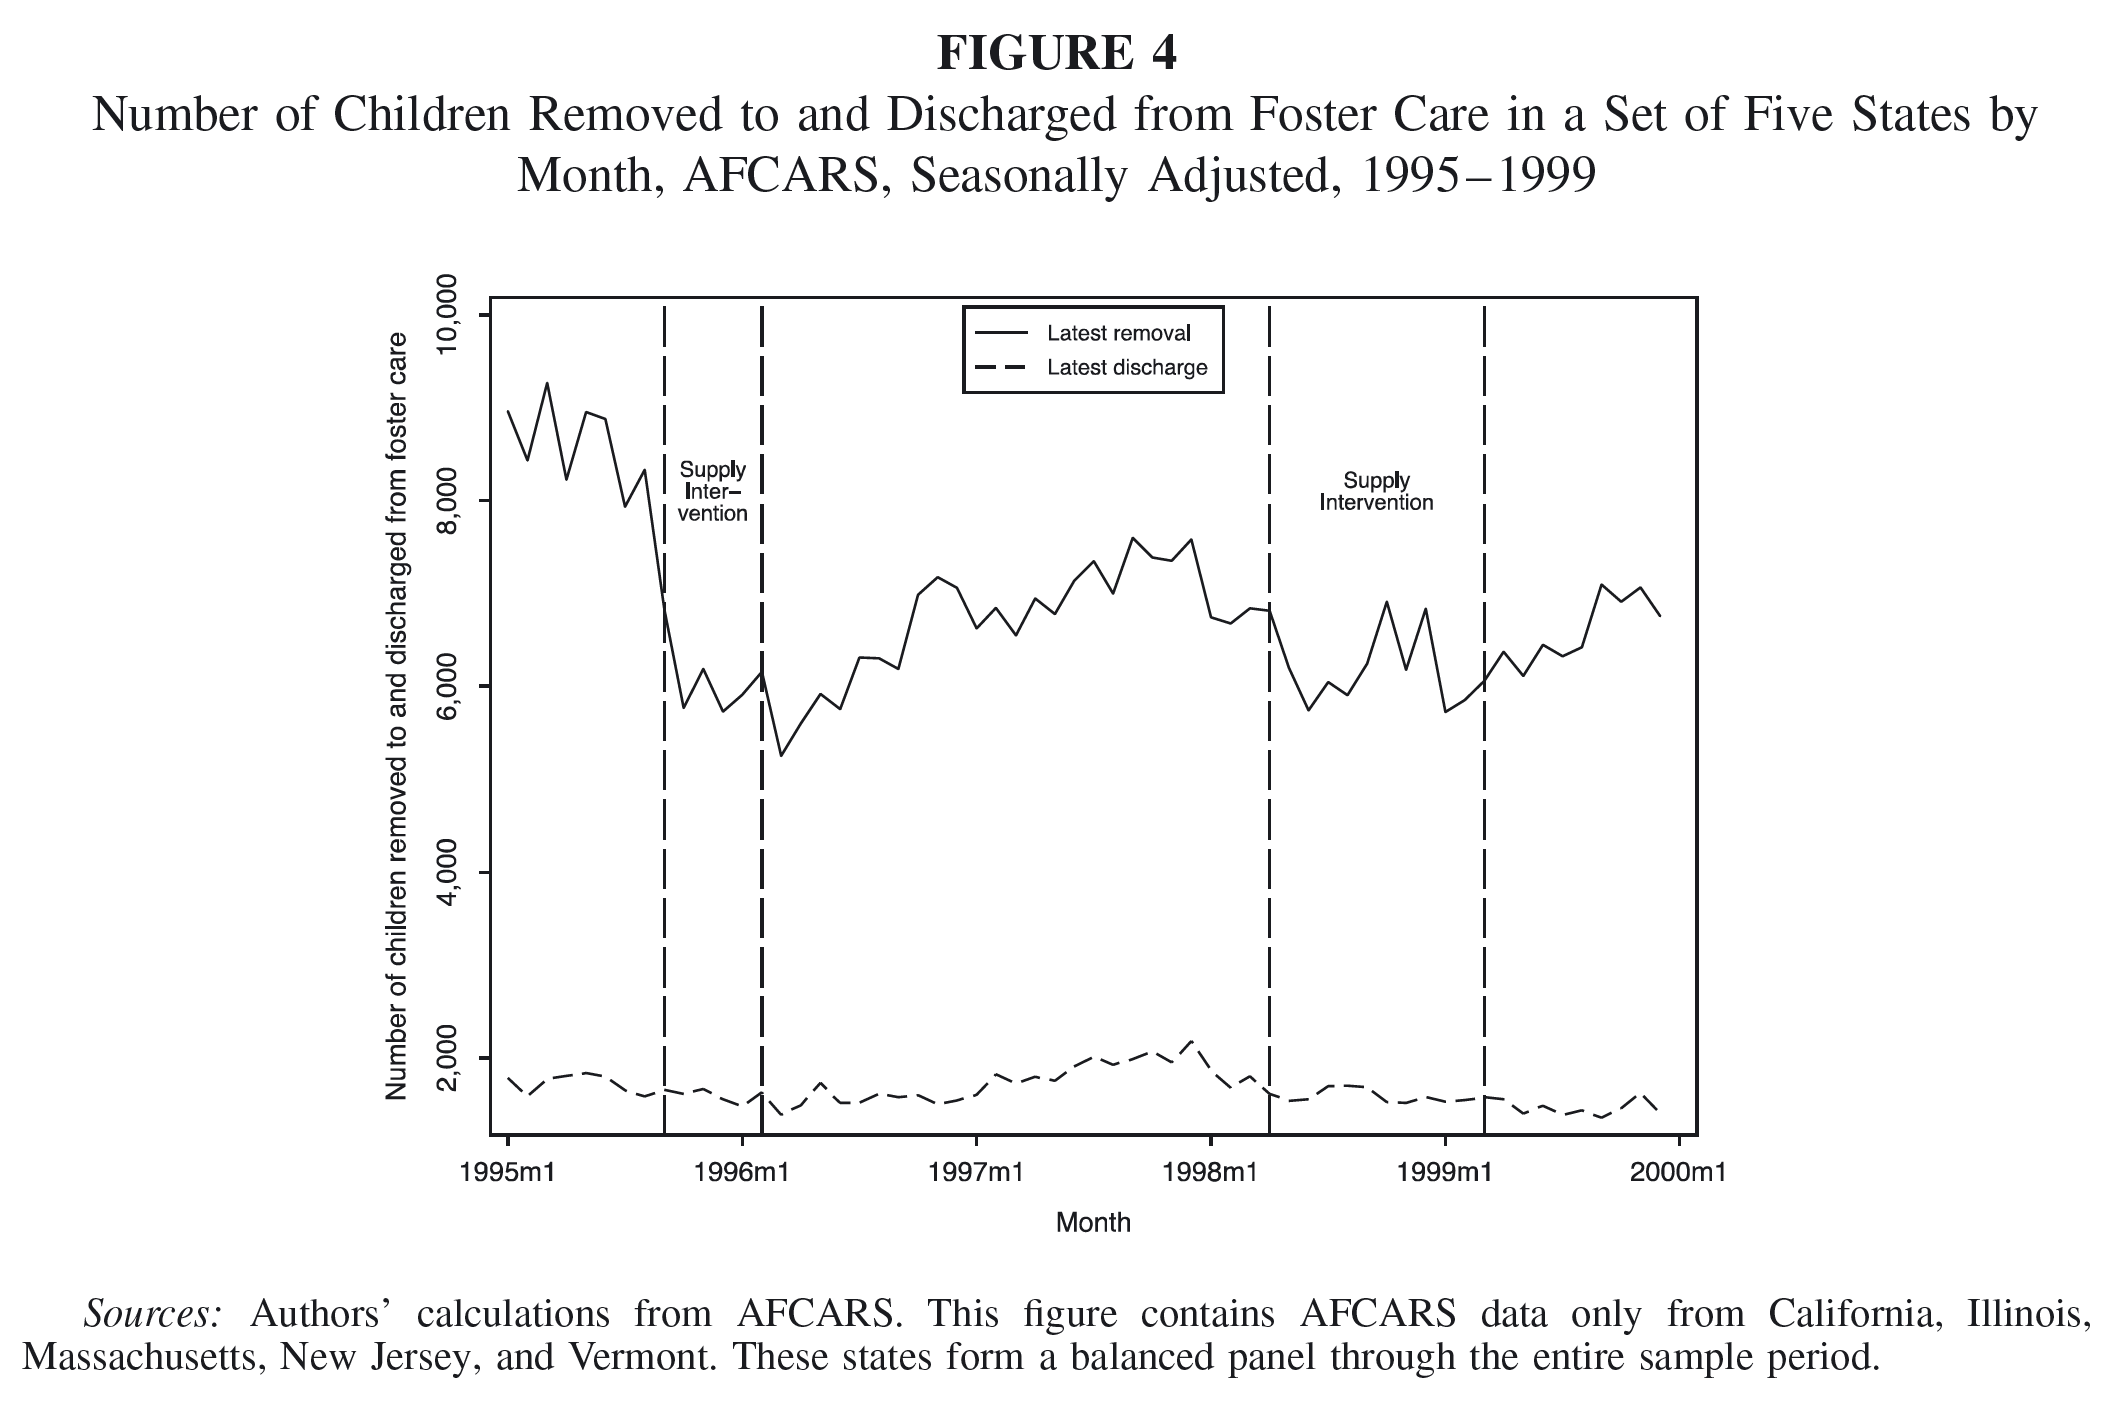
\includegraphics[scale=0.15]{./lecture_includes/keith_2.png}
	\end{figure}
	
\end{frame}

\begin{frame}{Tables}

\begin{enumerate}
\item Naive OLS model (though with heterogeneity this may not be informative of same parameter with IV)
\item Reduced Form
\item First stage
\item Weak instrument tests
\item IV model
\end{enumerate}

\end{frame}



\begin{frame}[plain]

\begin{table}[htbp]\centering
\scriptsize
\caption{OLS and 2SLS regressions of Log Earnings on Schooling}
\label{2sls_1}
\begin{center}
\begin{threeparttable}
\begin{tabular}{l*{2}{c}}
\toprule
\multicolumn{1}{l}{\textbf{Dependent variable}}&
\multicolumn{2}{c}{\textbf{Log wage}}\\
\multicolumn{1}{c}{}&
\multicolumn{1}{c}{OLS}&
\multicolumn{1}{c}{2SLS}\\
\midrule
educ                &       0.071***&       0.124** \\
                    &     (0.003)   &     (0.050)   \\
exper               &       0.034***&       0.056***\\
                    &     (0.002)   &     (0.020)   \\
black               &      -0.166***&      -0.116** \\
                    &     (0.018)   &     (0.051)   \\
south               &      -0.132***&      -0.113***\\
                    &     (0.015)   &     (0.023)   \\
married             &      -0.036***&      -0.032***\\
                    &     (0.003)   &     (0.005)   \\
smsa                &       0.176***&       0.148***\\
                    &     (0.015)   &     (0.031)   \\
\\
\midrule
\multicolumn{1}{c}{First Stage Instrument}\\
College in the county&               &       0.327***\\
Robust standard error &               &       0.082   \\
F statistic for IV in first stage&               &      15.767   \\
N                   &       3,003   &       3,003   \\
Mean Dependent Variable&       6.262   &       6.262   \\
Std. Dev. Dependent Variable&       0.444   &       0.444   \\
\bottomrule
\end{tabular}
\begin{tablenotes}
\tiny
\item Standard errors in parenthesis. * p$<$0.10, ** p$<$0.05, *** p$<$0.01
\end{tablenotes}
\end{threeparttable}
\end{center}
\end{table}

\end{frame}



	
%\begin{frame}[shrink=20,plain]

%	\begin{center}
%	\textbf{Other potentially interesting treatment effects}
%	\end{center}
	
%	\begin{itemize}
%	\item Another effect which we may be potentially interested in estimating is the familiar estimand, the average treatment effect on the treatment group (ATT)
%	\item \underline{Remark}: LATE is \emph{not} the same as ATT, though.
%		\begin{eqnarray*}
%		\underbrace{E[Y_i^1 - Y_i^0 | D_i=1]}_{ \mathclap{\text{ATT}} }&=& \underbrace{E[Y_i^1 - Y_i^0 | D_i^0 = 1]}_{ \mathclap{\text{Effect on always takers}}} P[D_i^0 = 1 | D_i = 1]\\
%		& &+ \underbrace{E[Y^1_i - Y^0_i | D_i^1>D_i^0]}_{ \mathclap{\text{Effect on compliers}} } P[D_i^1 > D_i^0, Z_i=1 | D_i=1]
%		\end{eqnarray*}
%	\item The average treatment effect on the treated, ATT, is a weighted average of the effects on always-takers and compliers.
%		\begin{itemize}
%		\item \underline{Question}: What are the weights? 
%		\end{itemize}
%	\item If there are no always takers we can, however, estimate ATT which is equal to LATE in that case. 
%	\end{itemize}
	
%\end{frame}




	
		
%\begin{frame}[plain]
%	\begin{center}
%	\textbf{Discussions and questions}
%	\end{center}

%	\begin{itemize}
%	\item When might we \emph{not} be interested in the local average treatment effect?
%		\begin{itemize}
%		\item \underline{Romneycare in Massachusetts examples}: If the compliance rate or treatment effects differ in the community than during some quasi-experimental expansion, are we more interested in LATE, ATT or ATE?
%		\item What might be other examples of this in economics?  In education?
%		\item This has a similar flavor to methodological questions regarding a study's ``external'' vs. ``internal validity''
%		\end{itemize}
%	\end{itemize}
%\end{frame}

%\begin{frame}[plain]
%\begin{center}
%\textbf{Discussions and questions}
%\end{center}

%\begin{itemize}
%	 \item What do we make of the fact that LATE is defined for an \emph{unobservable sub-population} (i.e., can't label all units in the population as compliers or noncompliers)?
%	 \item What do we make of the fact that IV identification is based on a set of untestable assumptions?
%		\begin{itemize}
%		\item For example: colonial settler mortality ($Z$) influences economic development ($Y$) \emph{only through} $Z$'s association with human capital accumulation rather than institutions, $D$ (Acemoglu, Johnson and Robinson, 2001).
%		\end{itemize}
%\end{itemize}

%\end{frame}
\subsection{Leniency design}

\begin{frame}{Leniency designs}

	\begin{itemize}
	\item Imagine the following:
		\begin{enumerate}
		\item A person moves through a pipeline and hits a critical point where treatment occurs as a result of some decision-maker
		\item There are many different decision-makers and you're assigned randomly to one of them
		\item Each decision-maker differs in terms of their \emph{leniency} in assigning the treatment
		\end{enumerate}
	\item Very popular in criminal justice bc of how often judges are randomly assigned to defendants (Kling 2006; Mueller-Smith 2015; Dobbie, et al. 2018) or even children to foster care case workers (Doyle 2007; Doyle 2008)
	\end{itemize}
\end{frame}

\imageframe{./lecture_includes/judge_fe.pdf}

\begin{frame}{Juvenile incarceration}

	\begin{itemize}
	\item Aizer and Doyle (2015) were interested in the causal effect of juvenile imprisonment on future crime and human capital accumulation
	\item Extremely important policy question given the US has the world's highest incarceration rate and prison population of any country in the world by a significant margin (500 prisoners per 100,000, over 2 million adults imprisoned, 4.8 million under supervision)
	\item High rates of incarceration extend to juveniles: in 2010, the stock of juvenile detainees stood at 70,792, a rate of 2.3 per 1,000 aged 10-19. 
	\item Including supervision, US has a juvenile corrections rate 5x higher than the next highest country, South Africa
	\end{itemize}
	
\end{frame}

\begin{frame}{Confounding}


		\begin{center}
		\begin{tikzpicture}
			[node distance=1.5cm]
		% nodes %
		\node[text centered] (e) {$e$};
		\node[below right of  = e, text centered] (y) {$Y$};
		\node[below left of = e, text centered] (d) {$D$};
 
		% edges %
		\draw[->, line width=1] (d) -- (y);
		\draw[dashed, ->] (e) -- (y);
		\draw[dashed, ->] (e) -- (d);
		\end{tikzpicture}
		\end{center}
		
		\begin{itemize}
		\item We are interested in the causal effect of juvenile incarceration ($D$) on life outcomes, like adult crime and high school completion
		\item But youth \emph{choose} to commit crimes, and that choice may be due to unobserved criminogenic factors like poverty or underlying criminal propensities which are themselves causing those future outcomes
		\end{itemize}
		

\end{frame}

\begin{frame}{Leniency as an instrument}

		\begin{center}
		\begin{tikzpicture}
			[node distance=1.5cm]
		% nodes %
		\node[text centered] (e) {$e$};
		\node[below right of  = e, text centered] (y) {$Y$};
		\node[below left of = e, text centered] (d) {$D$};
		\node[above left of = d, text centered] (z) {$Z$};
 
		% edges %
		\draw[->, line width=1] (d) -- (y);
		\draw[->, line width=1] (z) -- (d);
		\draw[dashed, ->] (e) -- (y);
		\draw[dashed, ->] (e) -- (d);
		\end{tikzpicture}
		\end{center}
		
		\begin{itemize}
		\item Aizer and Doyle (2015) propose an instrument - the propensity to convict by the judge the youth is randomly assigned
		\item If judge assignment is random, and the various assumptions hold, then the IV strategy identifies the local average treatment effect of juvenile incarceration on life outcomes
		\end{itemize}

\end{frame}


\begin{frame}{The Main Idea}

	\begin{itemize}
	\item ``Plausibly exogenous'' variation in juvenile detention stemming from the random assignment of cases to judges who vary in their sentencing
	\item Consider two juveniles randomly assigned to two different judges with different incarceration tendencies (Scott and Bob)
	\item Random assignment ensures that differences in incarceration between Scott and Bob are due to the judge, not themselves, because remember, they're identical
	\end{itemize}
\end{frame}

\begin{frame}{Data}

	\begin{itemize}
	\item 35,000 juveniles administrative records over 10 years who came before a juvenile court in Chicago (Juvenile Court of Cook County Delinquency Database)
	\item Data were linked to public school data for Chicago (Chicago Public Schools) and adult incarceration data for Illinois (Illinois Dept. of Corrections Adult Admissions and Exits)
	\item They wanted to know the effect of juvenile incarceration on high school completion (2nd data needed) and adult crime (3rd data needed) using randomized judge assignment (1st data needed)
	\item They need personal identifying information in each data set to make this link (i.e., name, DOB, address)
	\end{itemize}
	
\end{frame}

\begin{frame}{Preview of findings}

	\begin{itemize}
	\item Juvenile incarceration decreased high school graduation by 13 percentage points (vs. 39pp in OLS)
	\item Increased adult incarceration by 23 percentage points (vs. 41pp in OLS)
	\item Marginal cases are high risk of adult incarceration and low risk of high school completion as a result of juvenile custody
	\item Unlikely to ever return to school after incarcerated, but when they do return, they are more likely to be classified as special ed students, and more likely to be classified for special ed services due to behavioral/emotional disorders (as opposed to cognitive disability)
	\end{itemize}
	
\end{frame}

\begin{frame}{``Plausibly'' exogenous}

	\begin{itemize}
	\item Very common in these studies for the assignment to some decision-maker to be \emph{arbitrary} but not clearly random (i.e., not random no. generator)
	\item In this case, juveniles charged with a crime are assigned to a calendar corresponding to their neighborhood and calendars have 1-2 judges who preside over them
	\item 1/5 of hearings are presided over by judges who cover the calendar when the main judge can't, known as swing judges
	\item Judge assignment is a function of the sequence with which cases happen to enter into the system and judge availability that is set in advance
	\item No scope for which judge you see first; conversations with court administrators confirm its random
	\end{itemize}
\end{frame}

\begin{frame}{Structural equation}

\begin{eqnarray*}
Y_i = \beta_0 + \beta_1 JI_i + \beta_2 X_i + \varepsilon_i
\end{eqnarray*}where $X_i$ is controls and $\varepsilon_i$ is an error term.  In this, juvenile incarceration is likely correlated with the error term.

\bigskip

This is the ``long'' causal model. But note, from the prior DAG, we cannot control for $e$ because it is unobserved. But it is confounding the estimation of juvenile incarceration's effect on outcomes.

\end{frame}

\begin{frame}{Incarceration Propensity as an Instrument}

	\begin{itemize}
	\item The instrument is based on the randomized judge equalling the propensity to incarcerate from the randomly assigned judge
	\item ``Leave-one-out mean''$$Z_{j(i)} = \bigg ( \frac{1}{n_{j(i)} - 1} \bigg ) \bigg ( \sum_{k \neq i}^{n_{j(i)}-1} \widetilde{JI}_k \bigg )$$
	\item The $n_{j(i)}$ terms is the total number of cases seen by judge $k$, and $\widetilde{JI}_k$ is equal to 1 if the juvenile was incarcerated during their first case
	\item Thus the instrument is the judge's incarceration among first cases based on all their other cases
	\item It's basically a judge fixed effect given the likelihood two judges have precisely the same propensity is small
	\end{itemize}
\end{frame}

\begin{frame}{Information about the instrument}

\begin{itemize}
	\item There are 62 judges in the data, and the average number of initial cases per judge is 607
	\item Substantial variation in the data - raw measure ranges from 4\% to 21\%
	\item Residualized measure based on controls still has substantial variation from 6\% to 18\%
	\item Variation comes from two sources: variation among the regular (nonswing) judges (80\% of cases) and variation from the swing judges (20\% of cases)
\end{itemize}

\end{frame}

\begin{frame}{Distribution of IV}
	
	\begin{figure}
	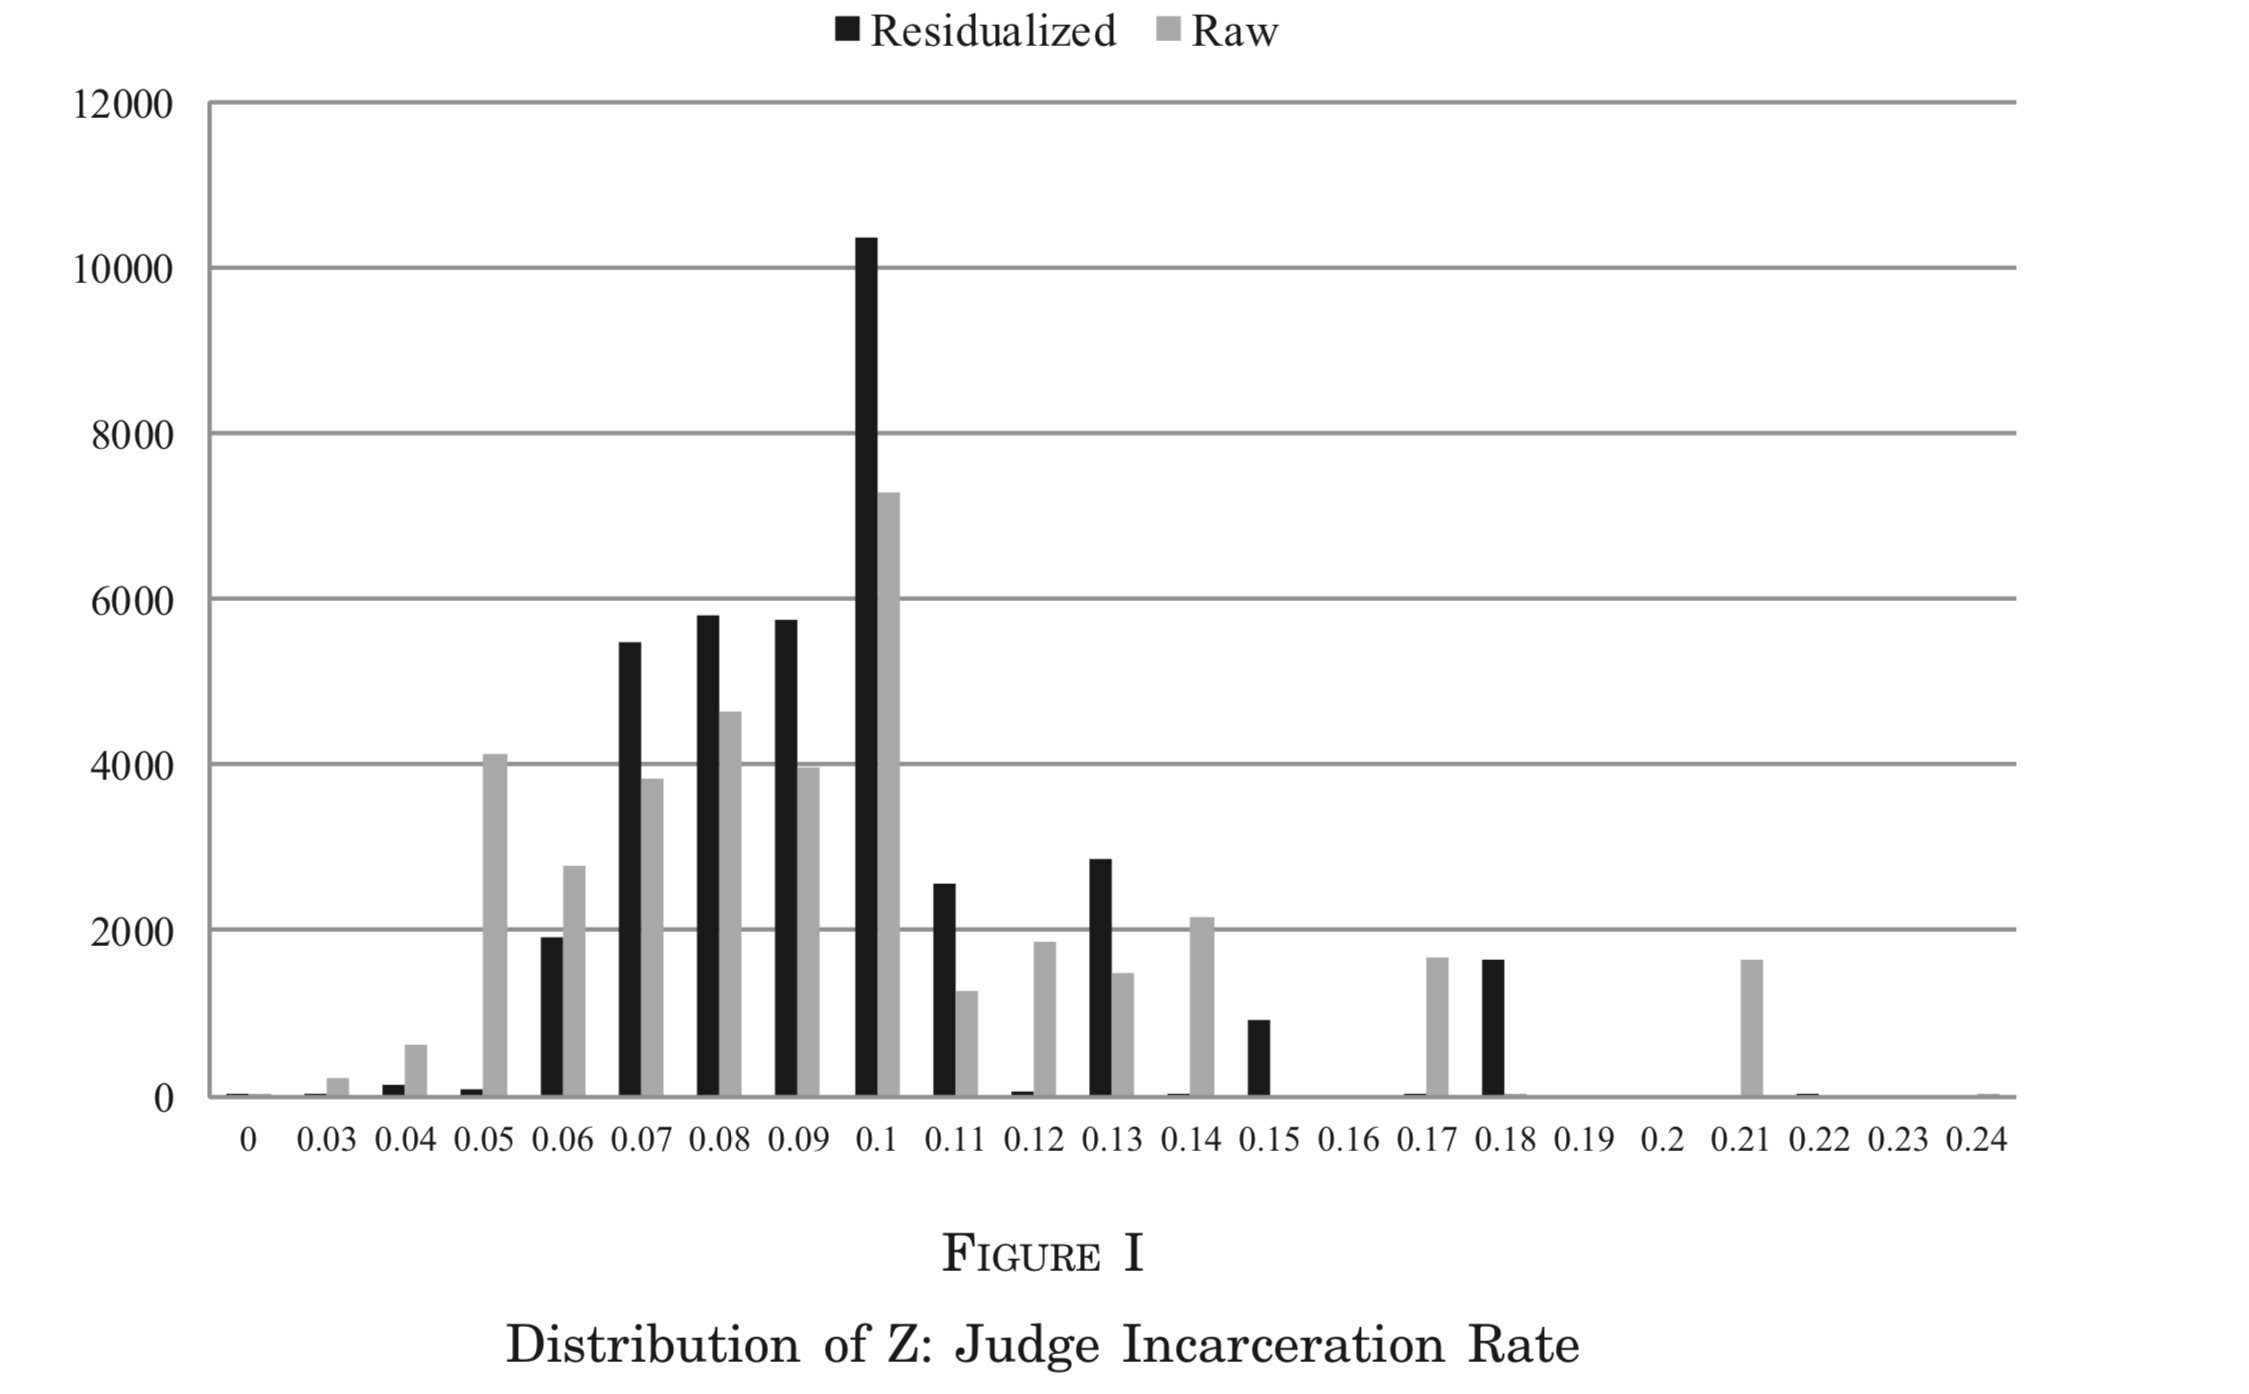
\includegraphics[scale=0.15]{./lecture_includes/iv.png}
	\end{figure}
\end{frame}
	
\begin{frame}{Balance test}
	
	\begin{figure}
	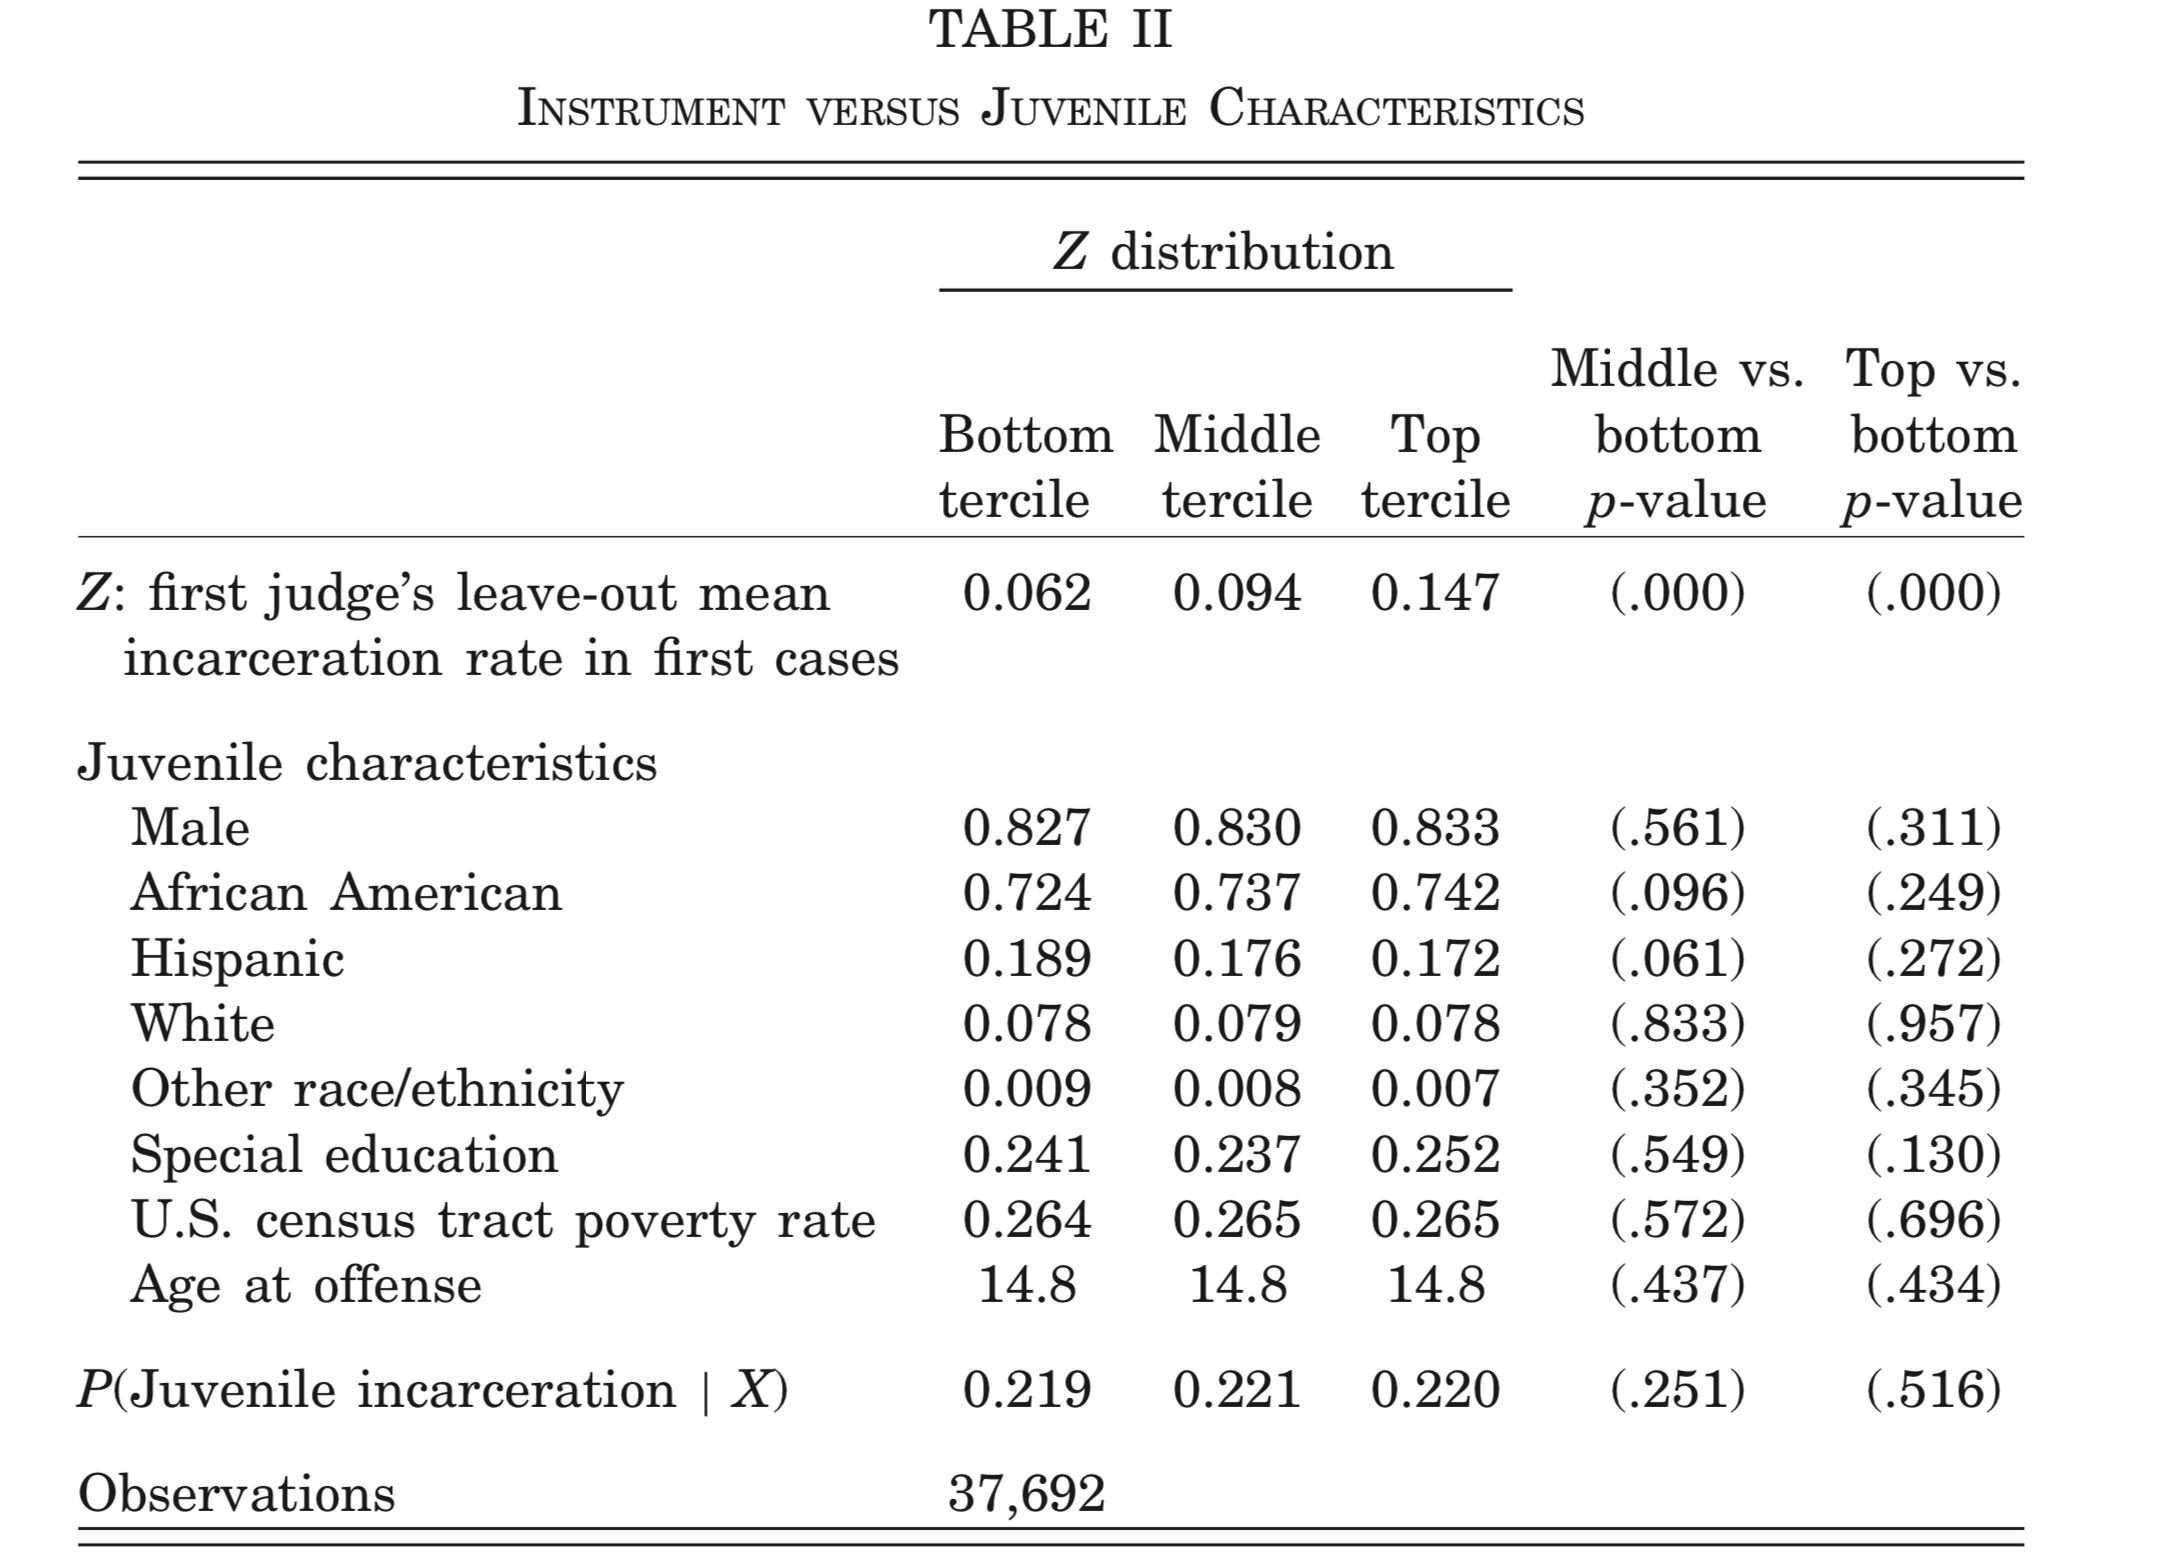
\includegraphics[scale=0.15]{./lecture_includes/balance.png}
	\end{figure}
\end{frame}

\begin{frame}{First stage}
	
	\begin{figure}
	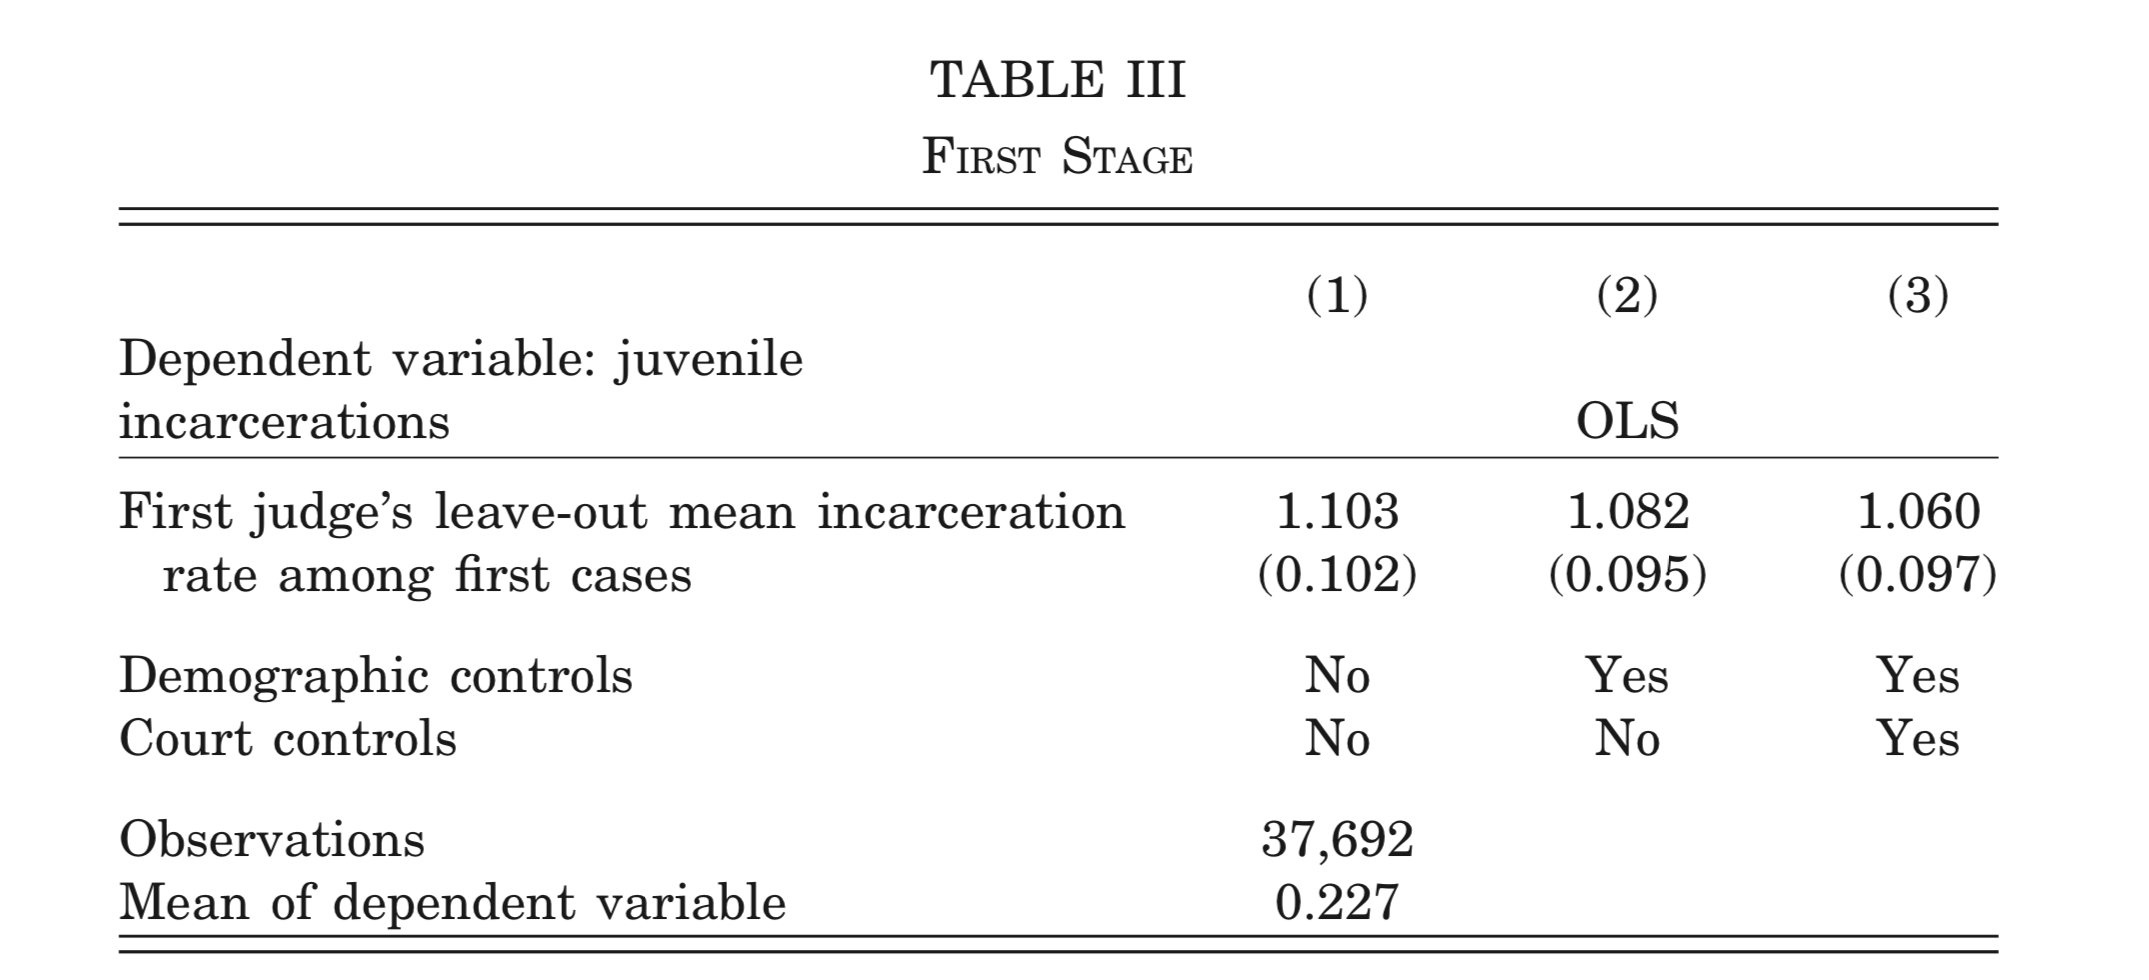
\includegraphics[scale=0.15]{./lecture_includes/firststage.png}
	\end{figure}
\end{frame}


\begin{frame}{High school completion}
	
	\begin{figure}
	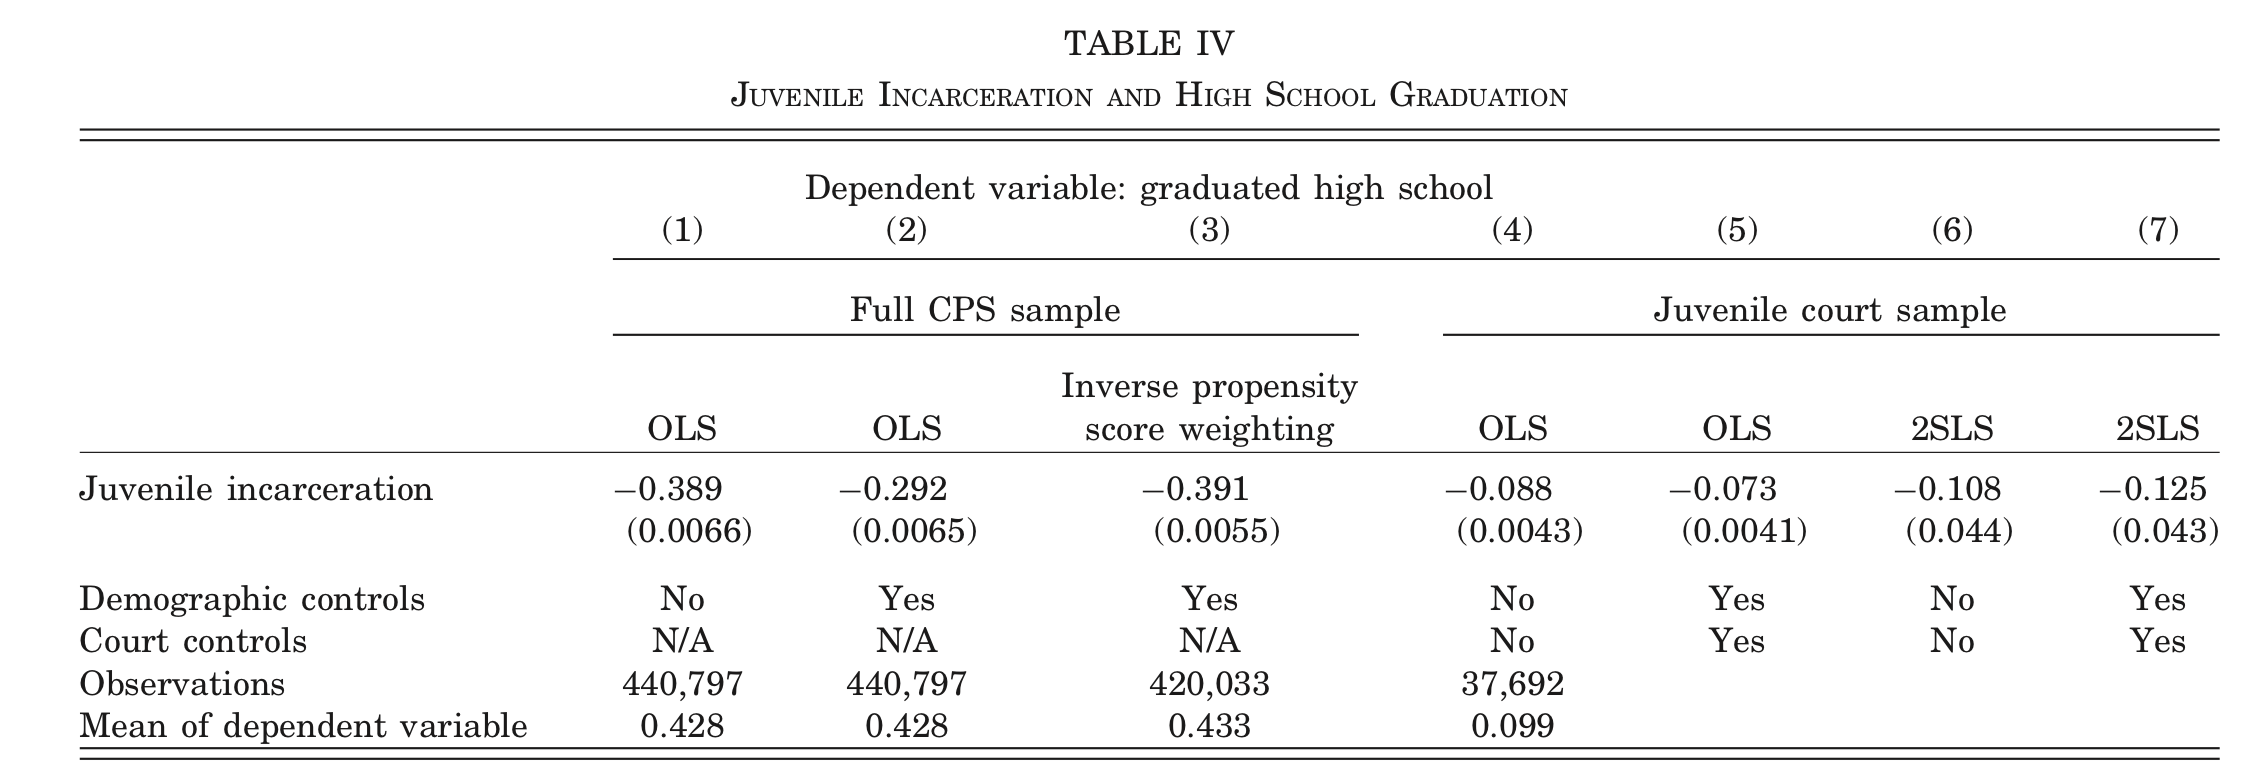
\includegraphics[scale=0.15]{./lecture_includes/highschool.png}
	\end{figure}
\end{frame}


\begin{frame}{Adult crime}
	
	\begin{figure}
	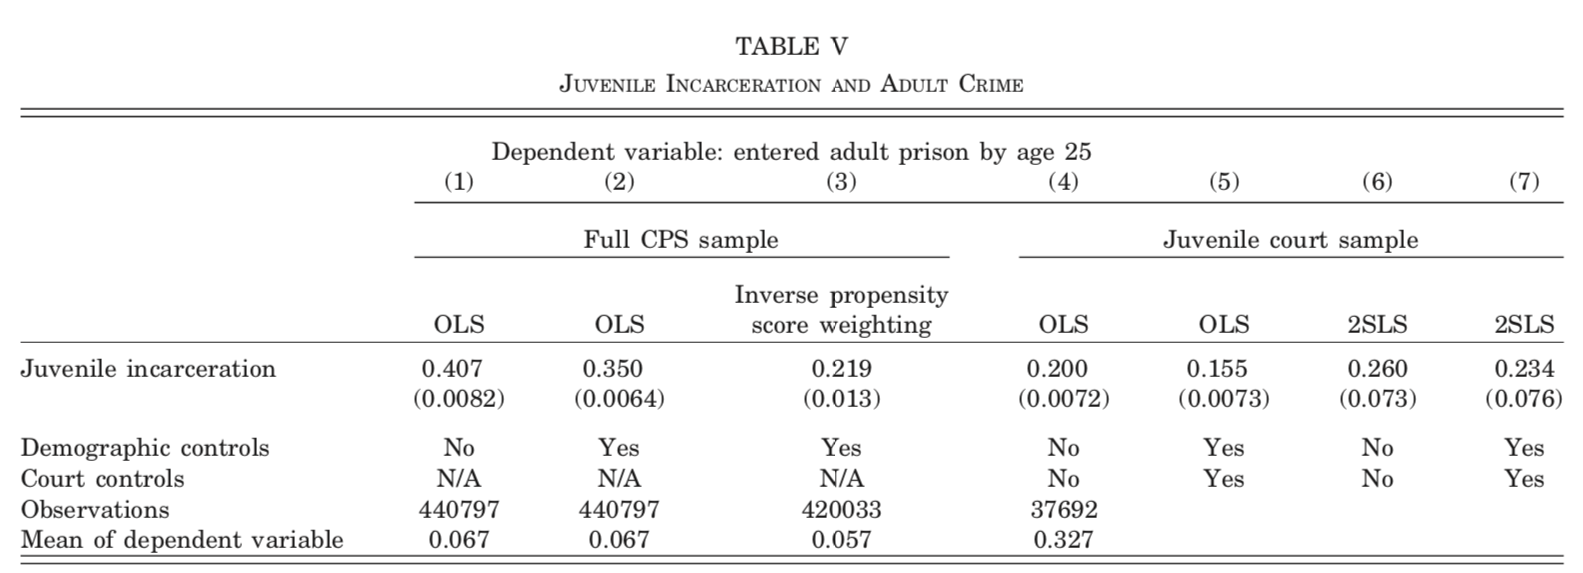
\includegraphics[scale=0.2]{./lecture_includes/adult_crime.png}
	\end{figure}
\end{frame}


\begin{frame}{Crime type}
	
	\begin{figure}
	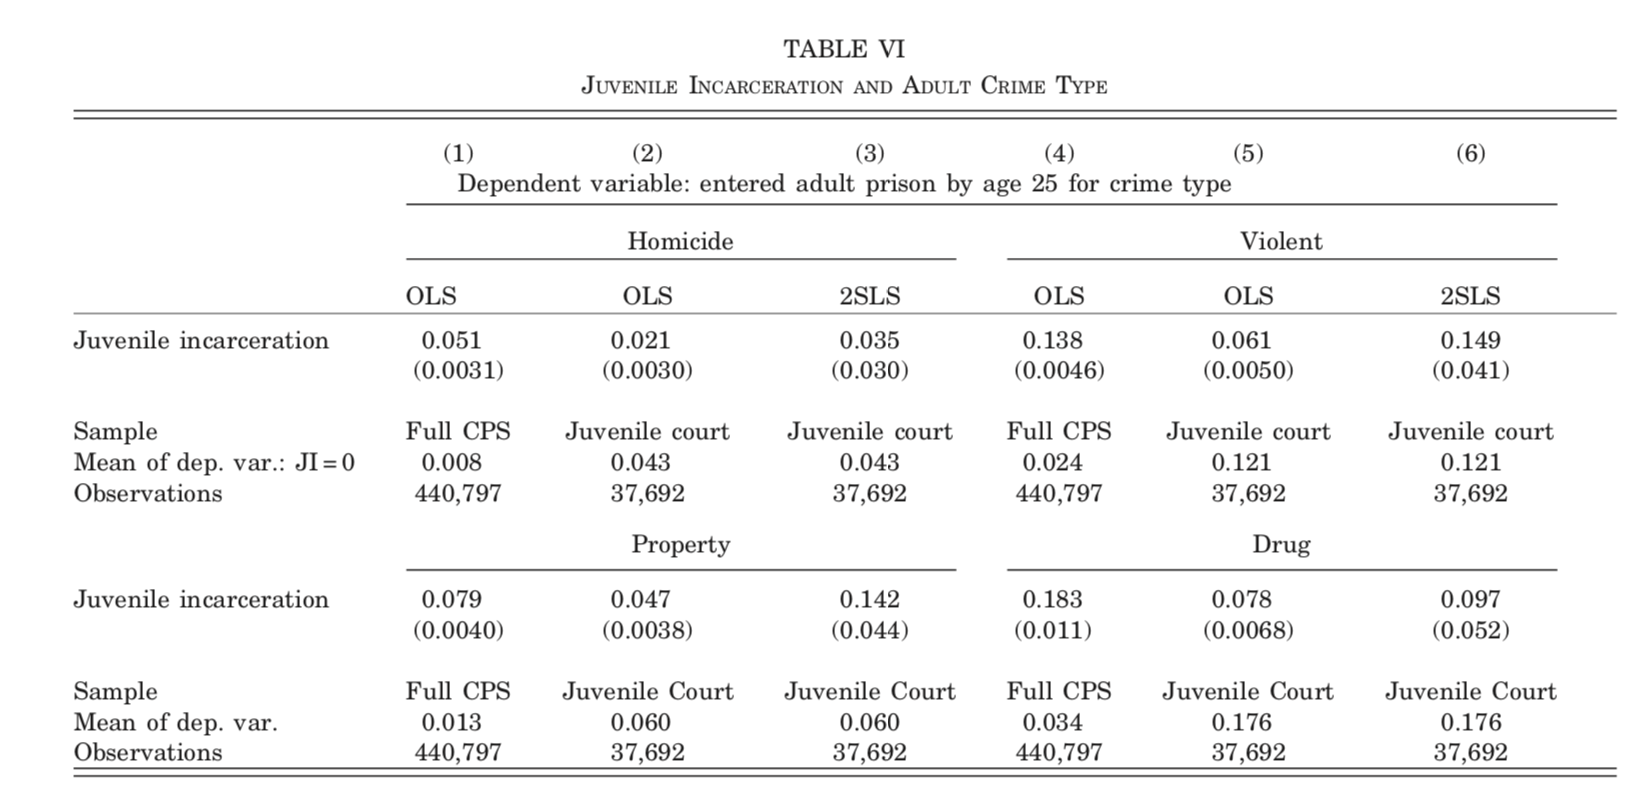
\includegraphics[scale=0.2]{./lecture_includes/crimetype.png}
	\end{figure}
\end{frame}


\begin{frame}{High school transfers}
	
	\begin{figure}
	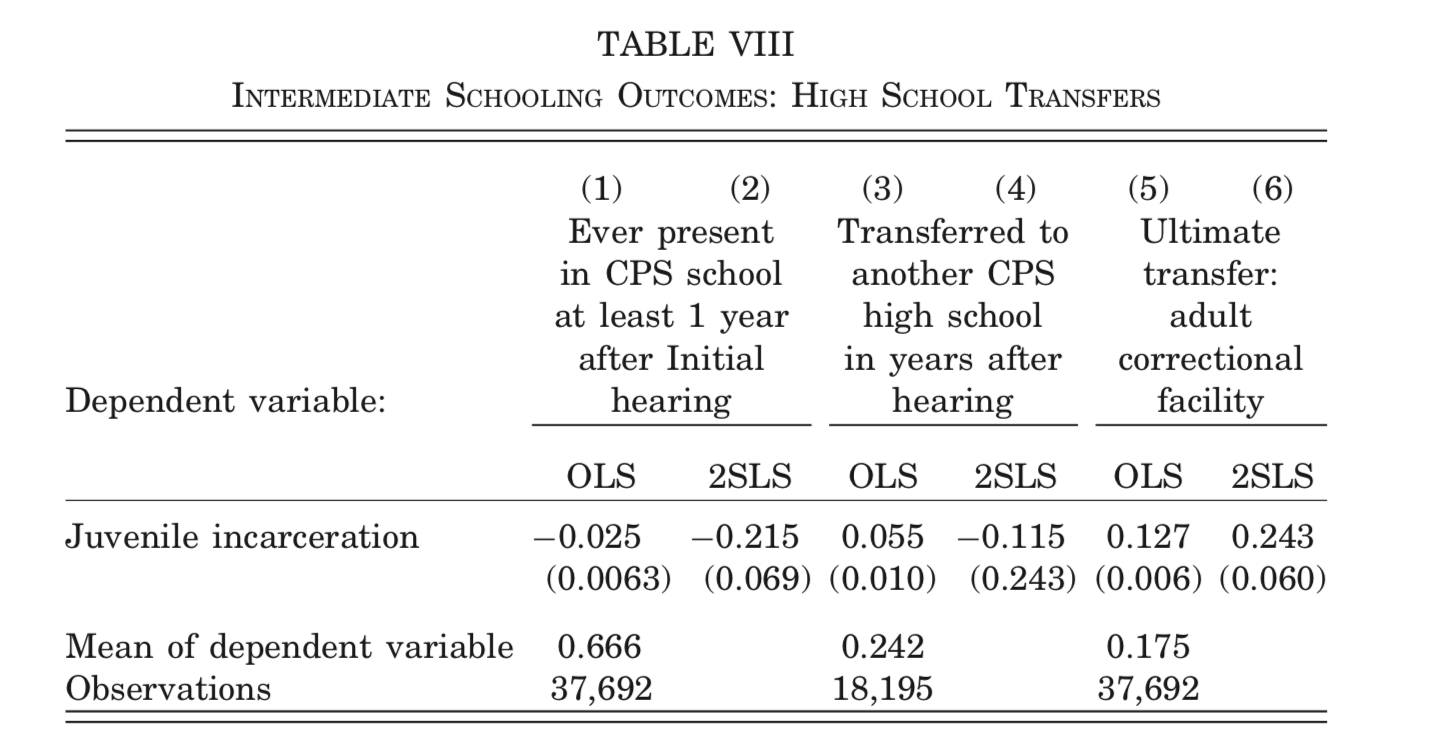
\includegraphics[scale=0.2]{./lecture_includes/transfers.png}
	\end{figure}
\end{frame}


\begin{frame}{Developing emotional problems}
	
	\begin{figure}
	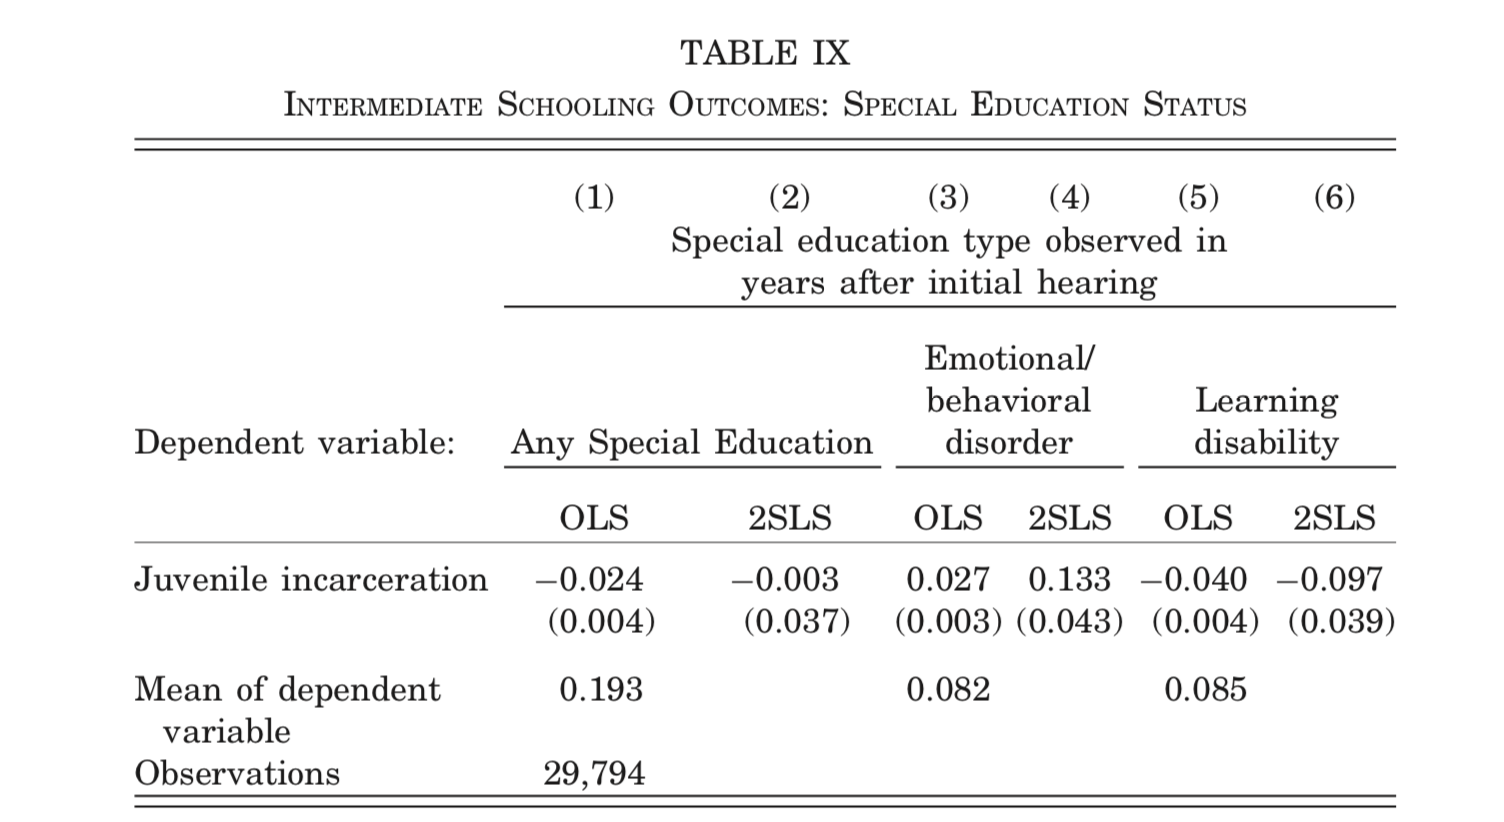
\includegraphics[scale=0.2]{./lecture_includes/disorder.png}
	\end{figure}
\end{frame}


\begin{frame}{Examples from our paper}

\begin{itemize}
\item Just accepted at JHR, ``Adverse Impacts of Mental Health Needs Assessment on Jail Outcomes: Evidence from Transition Age Youth and Adults'' with Cunningham, Seward, Clay and Vigliotti (randomized)

\item We investigated the effect of mental health needs scores on suicidality in jail and recidivism and explored possible mechanisms like length of stay

\item We also used a leniency design coming from randomized clinicians who scored on score of 0 to 3 the severity of their daily functioning

\item Rather than review the paper, I want to highlight the main exhibits of a leniency paper today

\end{itemize}

\end{frame}

\begin{frame}{Write down your structural equation}

First equation states your research question, not your instrumental variable strategy.  Let's consider a model in which an inmate $i$ at booking $b$ remains in jail longer, attempts suicide or recidivates based on interventions given in response to their mental health needs score, $Score_{ibt}$. 
\begin{equation}
    Y_{ibt} = \beta_0 + \beta_1 Score_{ibt} + \beta_2 X_{ibt} + \tau_t + \epsilon_{ibt},
    \label{eq:ols}
\end{equation}where $Y_{ibt}$ is the outcome of interest for individual $i$ in booking $b$ in month-year $t$: (1) length of stay, (2) suicide attempt, or (3) recidivism within a year of release.  The matrix $X_{ibt}$ contains baseline inmate and booking characteristics, $\tau_t$ is a vector of month-year dummies and $\varepsilon_{ibt}$ is an error term.  

\end{frame}

\begin{frame}{Present your instrument equation}

To isolate the effect of clinician scoring on the mental health needs score of inmate $i$ at booking $b$ in time $t$, we first estimate a linear model that includes a vector of month-of-year fixed effects. These fixed effects account for any county-wide trends that might affect mental health needs scores:
\begin{equation}
    \label{eq:residual}
    Score_{ibt} = \gamma_1 + \gamma_2 \tau_t + \varepsilon_{ibt} 
\end{equation}where $\varepsilon$ is an idiosyncratic error.  
\end{frame}

\begin{frame}{Present your instrument equation}

We then residualize the inmate's mental health needs score using the fitted coefficients from previous equation
\begin{equation}
    \label{eq:residual2}
    Score^{*}_{ibt} = Score_{ibt} - \widehat{\gamma_1} - \widehat{\gamma_2} \tau_{t}
\end{equation}
This residualized score isolates the part of the inmate's mental health needs score that is due to the clinician's scoring, independent of the month-of-year fixed effects. 

\end{frame}


\begin{frame}{Residualized leave-one-out mean IV}

We construct a measure of residualized clinician $c$ propensity to assign a high score $Z_{btc}$ as:

\begin{equation}
    \label{eq:instrument}
    Z_{btc} = \bigg(\frac{1}{n_{tc}-n_{itc}}\bigg) \bigg( \sum_{k=0}^{n_{it}} (Score^{*}_{ikt}) - \sum_{b=0}^{n_{itc}} (Score^{*}_{ibt}) \bigg),
\end{equation} where $n_{ct}$ is the number of cases seen by clinician $c$ in month-year $t$ and $n_{it}$ is the number of bookings of inmate $i$ seen by clinician $c$ in month-year $t$.

\bigskip

$Score^{*}_{ikt}$ is the residualized mental health needs score given by the clinician at time $t$, and $Score^{*}_{ibt}$ is the residualized score by inmates $i$.   In other words, we remove the residualized mental health needs score assignment of all of an inmate’s bookings seen by clinician $c$ in each month.

\end{frame}

\begin{frame}{Present the first stage equation}

We explore this positive association between the residualized leave-one-out-mean clinician scores and an inmate's own score by estimating the following linear probability model:
\begin{equation}
Score_{ibt} = \alpha + \pi Z_{btc} + X_{ibt} + \tau_t + \varepsilon_{ibt}\label{eq:firststage}
\end{equation}where $Score_{ibt}$ is the binary treatment variable (``classification score'') indicating whether an inmate received a mental health needs score of ``Moderate'' or ``Severe,'' and $Z_{btc}$ is a vector of the residualized leave-one-out-mean clinician score, $X_{ibt}$ is an array of pre-booking inmate characteristics, including race, sex, age at booking, whether they had a prior offense in the last year, the number of offenses per booking, $\tau_t$ are month-of-year fixed effects, and $\varepsilon_{ibt}$ is the inmate specific error term. Standard errors are two-way clustered by clinician and inmate.   

\end{frame}

\begin{frame}{First Stage Figures}
	\begin{figure}
             \centering
             \includegraphics[scale=0.25]{./lecture_includes/jhr_ivfig1}
	\end{figure}
\end{frame}


\begin{frame}{First Stage Tests}
	\begin{figure}
             \centering
             \includegraphics[scale=0.3]{./lecture_includes/jhr_ivfig2}
	\end{figure}
\end{frame}

\begin{frame}{First Stage Tests}
	\begin{figure}
             \centering
             \includegraphics[scale=0.3]{./lecture_includes/jhr_ivfig3}
	\end{figure}
\end{frame}

\begin{frame}{Balance Tests Showing Independence}
	\begin{figure}
             \centering
             \includegraphics[scale=0.2]{./lecture_includes/jhr_ivfig4}
	\end{figure}
\end{frame}

\begin{frame}{Average monotonicity tests}
	\begin{figure}
             \centering
             \includegraphics[scale=0.3]{./lecture_includes/jhr_ivfig5}
	\end{figure}
\end{frame}










\begin{frame}{2SLS and one instrument}

\begin{itemize}

\item When we have one endogenous variable and one instrument, we say the equation is ``just identified'' and if we have more instruments than endogenous variables we say it is ``overidentified''
\item 2SLS is best when just identified as weak instruments can be better controlled (and tests for it exist like reporting Anderson-Rubin CI as well as reporting appropriately robust F statistics like we saw)
\item Single instrument is also helped with visualization and balance tests which I think shouldn't be downplayed
\item But it has problems too which we will now explore

\end{itemize}

\end{frame}



\begin{frame}{Continuous instrument}

\begin{itemize}
\item LATE theorem (Imbens and Angrist 1994) references a binary treatment and binary instrument technically making tests for weak instruments easier with broad agreement 
\item But with a continuous instrument, things change in the leniency design -- for one, the LATE interpretation gets a little more challenging, and the monontonicity assumption more complicated
\end{itemize}

\end{frame}

\begin{frame}{Weak instruments}

\begin{itemize}
\item But it may even be that the just identified model is a bait and switch in the first place
\item Peter Hull and others, for one, have noted that the residualized leave-one-out mean used as the instrument is a collapsing of judge fixed effects into a single scalar as a quasi-propensity score (recall it's dimension reducing)
\item So really, the correct specification is judge fixed effects potentially, not the residualized leave-one-out-mean, and 2SLS has severe bias with multiple instruments
\end{itemize}

\end{frame}


\begin{frame}{Criticism of 2SLS: Over identification and bias}

\begin{itemize}
\item Even though the 2SLS model is just identified with residualized leave-one-out-mean, our instrument is actually multi-dimensional in the number of judges and with weak instruments, this creates finite sample bias for 2SLS due to \emph{many instruments}; see Sun's \texttt{manyweakiv} at \url{https://github.com/lsun20/manyweakiv}


\item To help pin this down, consider that the propensity score theorem which states the propensity score is a scalar based on dimension reduction in X (Rosenbaum and Rubin 1983)

\item This isn't really a just identified model so we should explore alternative models that are more appropriate for our data and design: we consider three
\end{itemize}

\end{frame}

\begin{frame}{Many instruments}

\begin{itemize}

\item High-dimensional instruments can arise when there is inherently large number of potentially relevant instruments or when it’s unclear how these instruments should be specified (e.g. dummy variables, interaction effects).
\end{itemize}

\end{frame}



\begin{frame}{Alternative to 2SLS: LIML}

\begin{itemize}
\item Two branches of IV: minimum distance IV (very old; limited information maximum likelihood) and ``two step'' procedures (Wald, 2SLS, JIVE, etc.)
\item If LATEs vary, then two step IV estimators like 2SLS estimate a convex combination of them
\item Minimum distances estimators like LIML may be outside the convex hull of the LATEs and may not be interpretable as causal
\item This calls into the question the use of LIML when there are large number of instruments, so not advised
\end{itemize}

\end{frame}

\begin{frame}{Alternative to 2SLS: JIVE}

\begin{itemize}
\item One popular alternative to the 2SLS model in these applications has been the jackknife IV estimator (JIVE) (Angrist, Imbens and Krueger 1999)

\item JIVE removes bias using leave-out first stage fits for each observation 

\item That is the fitted value for observation $i$ is $Z_i\widehat{\pi}_{i}$ where $\widehat{\pi}_i$ is an estimate that throws out observation $i$

\item The other appeal is that it can handle large number of instruments, but ironically \emph{not} large number of covariates

\end{itemize}

\end{frame}

\begin{frame}{Many control variables}

\begin{itemize}

\item The primary interest in an econometric analysis often lies in one or a few regressors, for which we want to estimate the causal effect on an outcome variable. 
\item However, to allow for a causal interpretation we need to control for confounding factors. 
\item Lasso-type techniques can be employed to appropriately select controls and thus improve the robustness of causal inference.

\end{itemize}

\end{frame}



\begin{frame}{Alternative to 2SLS: JIVE}

\begin{itemize}


\item Kolesar (2013) notes that in a finite sample, JIVE will be noisy and this estimation error will be correlated with the outcome since it depends on the treatment status of a particular person (unit of observation for me is an inmate).  

\item This will cause JIVE to be biased when the number of covariates is large as is the case in our context -- in my recent paper, for instance, I had 14 covariates and 84 time fixed effects. 

\item We face therefore a tradeoff between a set of time fixed effects that ensure conditional randomization and the biases created by large numbers of covariates for our JIVE estimator.  

\end{itemize}

\end{frame}





\begin{frame}{Alternative to 2SLS: UJIVE}

\begin{itemize}
\item Researchers therefore often accompany just identified 2SLS with another model that is robust for both large number of covariates and large number of instruments.  

\item First alternative is to estimate LATEs using the UJIVE estimator (Kolesar 2013)

\item UJIVE estimates are robust to a large set of \emph{covariates} and \emph{instruments} by excluding inmate $i$ from estimation, thus guaranteeing that the prediction error be uncorrelated with the outcome (Kolesar 2013)

\item This means that UJIVE estimates are consistent for a convex combination of LATEs even when we have a large number of covariates. 
\end{itemize}
\end{frame}


\begin{frame}{Alternative to 2SLS: UJIVE}

\begin{itemize}

\item You can implement this using Kolesar's matlab code \url{https://github.com/kolesarm/ivreg/blob/master/ivreg.m}, but it's giving us problems here so I can't report the results

\item You can also use Stata's \texttt{manyiv} and we will review that together, 

\item R: Kolesar's github does not yet have this updated for R \url{https://github.com/kolesarm/ivreg/tree/master}, see the ivreg.pdf

\end{itemize}

\end{frame}


\begin{frame}{Alternatives: LASSO}

\begin{itemize}
\item But there are also two machine learning selection IV models: 
    \begin{itemize}
    \item the post-double-selection model and 
    \item the post-lasso-orthogonalization method described by Chernozhukov (2015) which we loosely term our LASSO and post-LASSO models, respectively.  
    \end{itemize}
\item We use the Stata command \texttt{lassopack} for its implementation 
\end{itemize}

\end{frame}

\begin{frame}{Why pdslasso?}

\begin{itemize}
\item \texttt{pdslasso} and \texttt{ivlasso} are routines for estimating structural parameters in linear models with many controls and/or many instruments. 
\item The routines use methods for estimating sparse high-dimensional models, specifically the LASSO and the square-root-LASSO (Belloni et al. 2011, 2014).
\item Purpose of \texttt{pdslasso}  is to improve causal inference when the aim is to assess the effect of one or a few (possibly endogenous) regressors on the outcome variable. 
\item \texttt{pdslasso}  allows to select control variables and/or instruments.
\end{itemize}

\end{frame}

\begin{frame}{LASSOPACK}


\begin{itemize}
\item These estimators can be used to select controls (pdslasso) or instruments
(ivlasso) from a large set of variables (possibly numbering more than the
number of observations), in a setting where the researcher is interested in
estimating the causal impact of one or more (possibly endogenous) causal
variables of interest.
\item Two approaches are implemented in pdslasso and ivlasso: (1) The "post-
double-selection" (PDS) methodology of Belloni et al. (2012, 2013, 2014,
2015, 2016). (2) The "post-regularization" (CHS) methodology of
Chernozhukov, Hansen and Spindler (2015). For instrumental variable
estimation, ivlasso implements weak-identification-robust hypothesis tests
and confidence sets using the Chernozhukov et al. (2013) sup-score test.
\end{itemize}

\end{frame}






\begin{frame}{Results}
	\begin{figure}
             \centering
             \includegraphics[scale=0.3]{./lecture_includes/jhr_ivfig6}
	\end{figure}
\end{frame}



\subsection{Marginal Treatment Effects}

\begin{frame}{Marginal treatment effects and judge IV}

\begin{itemize}

\item Increasingly common to see people go from estimating LATE effects with judges to MTE and then even to ATT, ATE and ATU
\item Literature goes back to early 2000s by Ed Vycatil and Jim Heckman in a series of papers
\item Works only with a continuous instrument, which you have with the residualized leave-one-out mean

\end{itemize}

\end{frame}


\begin{frame}{Marginal Treatment Effects}
       \begin{columns}
          \column{0.38\linewidth}
             \centering
             \includegraphics[height=5.25cm, width=4.5cm]{./lecture_includes/labour_mte.png}
           \column{0.65\linewidth}
		\begin{itemize}
	\item Cornelissen, et al. (2016) is a phenomenal review of this literature
	\item I've found this literature really fascinating
	\item If there is heterogeneity in unobservables
	\item To get a distribution of treatment effects
	\item Calculate aggregate parameters like the ATE
		\end{itemize}
         \end{columns} 
    \end{frame}





\begin{frame}{Marginal treatment effects}

What assumptions do we need? 
    	\begin{itemize}
	\item Heckman and Vytacil (2005, 2006, 2007, etc.) show that all policy relevant parameters (e.g., ATE, ATT, ATU) can be reconstructed using weighted averages over the MTE
   	\item Technically you can identify LATE with average monotonicity, but you need strict for MTE (new AER by Frandsen, Lefgren and Leslie forthcoming)
    	\item Additive separability of treatment effects (i.e., unobserved based on covariates plus observed heterogeneity)
    	\item Only required if not full support, and we don't have full support
	\end{itemize}

\end{frame}

\begin{frame}{Marginal treatment effects}

\begin{itemize}

\item Rooted in the LATE revolution in the 1990s focused on identifying models with heterogenous treatment effects
\item Imbens and Angrist are known for the LATE theorem and clarified interpretation of IV estimates
\item Heckam and Vytlacil, Card and others proposed a control function approach as an alternative to linear IV which under stronger assumptions than IV would allow the estimation of the ATE (which IV could not do)
\end{itemize}

\end{frame}

\begin{frame}{Marginal treatment effects}

\begin{itemize}
\item Marginal treatment effect (MTE) appears in the late 80s in the context of a switching regression model where "marginal gain" was the gain from treatment for people who were shifted into (or out of) treatment status by a marginal change in the cost of the treatment (which was the instrument)

\item Heckman and Vytlacil in four articles from 1999 to 2007 define the MTE as the ``gain from treatment for individuals shifted into treatment or out of treatment by a marginal change in the \emph{propensity score} (i.e., the predicted probability of treatment which is a function of the instrument)
\item They then develop nonparametric estimation methods and clarify the connection of the switching regime self selection model and of MTE with IV and LATE

\end{itemize}

\end{frame}

\begin{frame}{Marginal treatment effects}

\begin{itemize}
\item Since it's familiar to the audience, I'll focus on recidivism from the mental health paper I mentioned not suicide
\item In our context, we could have explored the heterogeneity in treatment effects across inmates' underlying mental illness proxied by the propensity score
\item Consider the following equations decomposing an inmate $i$'s potential recidivism into the conditional means of potential outcomes, $\mu^j(X_i)$, based on inmate characteristics $X_i$ as well as deviations from the mean $U_i^j$
\end{itemize}

\begin{eqnarray*}
Y_i^0 &=& \mu^0(X_i) + U_i^0 \\
Y_i^1 &=& \mu^1(X_i) + U_i^1 
\end{eqnarray*}

\end{frame}

\begin{frame}{Selection into treatment}


Mental illness scores are assigned based on an individual latent index threshold in which the net benefits of ``severe mental illness'' (obviously odd way of putting it) are exactly equal to
\bigskip
\begin{eqnarray*}
D_i^* = \mu^D(X_i,Z_i) - V_i
\end{eqnarray*}where $X_i$ and $Z_i$ are the inmate's observed determinants of treatment choice, but $Z_i$ is the instruments, and $V_i$ the unobserved characteristics that makes treatment choice less like (``unobserved resistance to treatment'')

\bigskip

Assignment to a severe mental illness score (low functioning) occurs when $D_i^*>0$ otherwise they are classified as high functioning

\end{frame}

\begin{frame}{Selection into treatment}

Or to be simpler about it, this is our "selection into treatment" equation meaning a person's treatment status is either 0 or 1 depending on the right hand side being positive or negative:

\begin{eqnarray*}
D_i^* = \mu^D(X_i,Z_i) - V_i
\end{eqnarray*}

\bigskip

$D_i=1$ if $D_i*\geq 0$,  otherwise $D_i=0$.  $V_i$ is an i.i.d. error term indicating unobserved heterogeneity in the propensity for treatment.  The error term $V_i$ enters the selection equation with a negative sign, it embodies unobserved characteristics that make individuals \emph{less} likely to receive treatment. As I said on the other page, people call it ``unobserved resistance to treatment'' or even ``distaste''.  

\end{frame}


\begin{frame}{Selection and expected gains}

\begin{itemize}
\item Very common for people in this literature to use language about ``selection based on gains'' as in choosing the treatment bc they expect to gain from it
\item In our context, we don't think you can take that literally because their moderate to severe mental illness is doing the choosing
\item We treat ``choice'' and ``moderate to severe mental illness'' are treated as synonyms, but that's just in our context
\end{itemize}

\end{frame}

\begin{frame}{Selection}

\begin{itemize}
\item The directions on our variables can be a little hard to interpret because for us higher values of $\mu_D(X,Z)$ basically cause them to get a severe mental illness score, but they correspond to worse symptoms
\item When the therapist believes the inmate's functioning is above her own reservation threshold for that inmate, $V_i$, the evaluator assigns a high score which assigns him to a high severe mental illness score
\end{itemize}

\end{frame}

\begin{frame}{Selection}

\begin{itemize}
\item Indifference condition is $\mu_D(X,Z)=V$, and thus when $D^*>0$, $\mu_D(X,Z)>V$, and the therapist assigns him to a severe mental illness score
\item We then apply the cdf of $V$ to this inequality to get $F_V(\mu^D(X_i,Z_i)) \geq F_V(V_i)$ which bounds both sides b/w 0 and 1
\item The left side is the propensity score (i.e., the conditional probability of treatment) which is $p_i(X_i,Z_i)$ and the right is the quantiles of the distribution of the unobserved resistance to treatment, $U_i^D$
\item Rewrite the selection equation  as $p_i(X_i,Z_i) \geq U_i^D$ which means an inmate $i$ selects into treatment when their propensity score is greater than their unwillingness to participate due to their slightly higher functioning
\end{itemize}

\end{frame}


\begin{frame}
\frametitle{Some sources of confusion I had}

\begin{itemize}
\item So it may help if you replace the phrase ``high propensity score / low resistance to treatment'' with ``moderate to severe mental illness'' (high scores)
\item If I have schizophrenia with extreme displays of psychosis, then I am \textbf{less} resistance to treatment because the treatment is a high score, and I will almost certainly get a high score (high propensity score)
\item If I come in with depression but am functional, my score is lower and so I both have a lower propensity score \emph{and} therefore have a \emph{higher} resistance to treatment
\item Note the subtle language: ``propensity score'' and ``resistance to treatment'' are reversed -- people with less resistance have higher propensity scores because their illness is so severe
\end{itemize}

\end{frame}



\begin{frame}{Switching equation}

Write down the choice of either potential outcome according to which treatment was chosen using a switching equation

\begin{eqnarray*}
Y_i &=& D_iY_i^1 + (1-D_i)Y_i^0 \\
Y_i &=& Y_i^0 + (Y_i^1 - Y_i^0)D_i
\end{eqnarray*}which is a regression equation.  If we substitute our earlier potential outcomes into this we get:

\begin{eqnarray*}
Y_i &=& \mu^0(X_i) + D_i(\mu^1(X_i) - \mu^0(X_i) + U_i^1 - U_i^0) + U_i^0
\end{eqnarray*}

\end{frame}

\begin{frame}{Assumptions}

\begin{block}{\textbf{Assumption 1: Conditional Independence}}
$(U^1,U^0,V) \perp\!\!\!\perp Z | X$

\bigskip

Implied by standard LATE assumptions (e.g., non-zero first stage, exclusion, SUTVA, monotonicity) are equivalent to some representation of a choice equation.  This is no more restrictive than the LATE model. And that could be enough, except that it requires full support of the propensity scores in both treated and untreated samples for all values of $X$ and in practice this rarely holds. So most proceed with a stronger assumption.

\end{block}

\end{frame}


\begin{frame}{Assumptions}

\begin{block}{\textbf{Assumption 2: Separability}}
$E[U^j|V,X] = E[U^j|V]$

\bigskip

It's a strong assumption.  First, the MTE is identified over the common support, unconditional on $X$.  Second, the MTEs are additively separable in $U^D$ and $X$. The intercept, but not the slope, is a function of $X$. 


\end{block}

\end{frame}




\begin{frame}
\frametitle{Steps}

\begin{enumerate}
\item Estimate the propensity score using logit (here issues of common support arise as we want it across all cells of Z)
\item Model recidivism as a function of covariates and propensity score with second degree polynomials
\item Calculate the derivative of $\widehat{recidivism}$ with respect to the propensity score and plot it as a curve
\end{enumerate}

\bigskip

Since we don't have full support, we rescaled the weights so that they integrate to one over the trimmed sample so that we can calculate different weighted averages of the MTEs


\end{frame}



\begin{frame}
\frametitle{Calculating aggregates}

\begin{itemize}
\item ATE is the equally weighted average over the entire MTE curve, ATT as a weighted average over the left group of ``low resistance, high propensity score'', and ATU as the weighted average of the right group of (``high resistance, low propensity'')
\item Downward slope means selection on unobserved returns to receiving a mental illness score (i.e., ATT$>$ATE$>$ATU)
\item Upward slope means the reverse (i.e., ATU$>$ATE$>$ATT)
\end{itemize}

\end{frame}

\begin{frame}{Common support}

    \includegraphics[width=\textwidth]{./lecture_includes/common_support_recid.png}

\end{frame}

\begin{frame}{MTE and aggregate parameters for recidivism}

    \includegraphics[width=\textwidth]{./lecture_includes/mte_recid__2.png}

\end{frame}
\subsection{Covariates}

\begin{frame}{IV with covariates}

\begin{itemize}
\item What if you think you need to control for covariates?  Can't you just control for it in your 2SLS specification? But how?
\item Blandhol, et al. (2022) as well as Stoczynski (2021) bring up some issues with typical 2SLS specifications with covariates
\item This is a decently sized literature going back at least to Abadie (2003), Frolich (2007), as well as to a degree Imbens and Angrist (1995)
\item The punchline is that controlling for covariates can be somewhat hazardous when using 2SLS
\end{itemize}


\end{frame}


\begin{frame}{Saturated regression models}

\begin{itemize}
\item Remember Angrist and Krueger's QoB instrument specification where they interacted Z with region of birth and year of birth?  This was almost entirely a saturated model (they didn't interact Z with age I don't think)
\item Saturated models are the full set of interactions on all discrete covariates as well as each one independently 
\end{itemize}

\bigskip

\begin{quote}
``Saturated regression models are regression models with discrete explanatory variables, where the model includes a separate parameter for all possible values taken on by the explanatory variables.'' (Angrist and Pischke 2009, p. 48-49)
\end{quote}

\end{frame}


\begin{frame}{Identification with covariates and 2SLS}

\begin{itemize}
\item We have to modify independence and exclusion (which isn't all that surprising), but we also have to introduce new types of first stage and common support assumptions
\item Assume conditional independence since we're controlling for X, exclusion conditional on X, positive correlation with covariates and treatment
\item Common support assumptions: there are units with $Z=1$ across distribution of X and units in both treatment and control across X 
\item The last two parts of that requires that there is variation in the instrument as well as a distinct number of compliers and defiers at every value of covariates
\end{itemize}

\end{frame}

\begin{frame}{2SLS estimand with covariates}

If you assume this and monotonicity, then Sloczyn'ski (2021),  Angrist and Imbens (1995) and Kolesar 2013) shows that a saturated 2SLS model identifies a convex combination of conditional LATEs with weights equal to the conditional variance of the first stage
\begin{eqnarray*}
\delta_{2SLS} = \frac{E[\sigma^2(X) \cdot \tau(X) ]}{E[\sigma^2(X)]}
\end{eqnarray*}where $\sigma^2$ is $E \bigg [ (E[D|X,Z] - E[D|X] )^2 | X \bigg ]$ and $\tau(x)$ is the conditional LATE.  Notice the variances weighting the conditional LATEs

\end{frame}



\begin{frame}{Covariates in 2SLS models}

\begin{itemize}
\item So the Angrist and Imbens (1995) approach to interacting the instrument with all possible dummies combining covariates in a saturated 2SLS model is not only sufficient to recover weighted combination of LATEs -- it's also necessary
\item But though Angrist and Imbens (1995) did it this way, it's very rare to see covariates controlled for in a nonparametric way like this because overidentification with 2SLS raises issues with weak instruments
\end{itemize}

\begin{quote}
`` Bound, Jaeger and Baker (1995) write, "[our results] indicate that the common practice of adding interaction terms as excluded instruments may exacerbate the [weak instruments] problem.''
\end{quote}
\begin{itemize}
\item Another possibility is to run first stages for every value of X combination (these get huge quickly) and weight them so as to avoid curse of dimensionality issues
\end{itemize}

\end{frame}



\begin{frame}{Saturate and weight}

\begin{itemize}
\item Only one that isn't is the saturate and weight method which requires interacting dummies for values of continuous $X_k$ with all $X_{k'}$ which in a finite sample runs into curse of dimensionality
\item Some cells won't have any variation in $Z$ conditional on $X$
\item They show it's necessary and sufficient for estimate to be weighted average over all individual LATEs, otherwise negative weights enter
\end{itemize}

\end{frame}

\begin{frame}{Covariates going forward}

\begin{itemize}
\item When all covariates are discrete, then the Angrist and Imbens (1995) saturated method recovers convex combination of conditional LATEs
\item 2SLS will in general reflect treatment effects for compliers and always/never takers, and some of the treatment effects for the always/never-takers will necessarily be negatively weighted
\item Sloczyn'ski (2021) introduces a new procedure called ``reordered IV'' but it doesn't guarantee that the resulting estimand will be similar to the unconditional LATE
\item There are a variety of alternatives to 2SLS like Abadie (2003), which uses a propensity score (for Z) to construct ``kappa weights'' 
\end{itemize}

\end{frame}

	




\begin{frame}{Concluding remarks}

	\begin{itemize}
	\item Identifying causal effect without an instrument is likely not possible given the deep selection issues associated with crime as a child and adult
	\item Leniency designs are everywhere, even in tech, but you need to know how to look for them
	\item Bottleneck, influential decision-makers, discretion - these are the three elements of the design
	\end{itemize}

\end{frame}


\subsection{Price elasticity of demand}

\begin{frame}{Supply and Demand}

\begin{itemize}
\item Instrumental variables was developed in the 1920s largely to address problems created by supply and demand
\item Demand curves are causal functions, but so are supply curves
\item We do not observe all the prices and quantities to be able to calculate the slope or shape of the demand curve because we only observe the ``realized prices and quantities'' in equilibrium
\item But if we did know the price elasticity of demand, we could set more optimal policies like tax policy or profit maximization
\end{itemize}

\end{frame}

\begin{frame}{Supply and Demand}
	
	\begin{figure}
	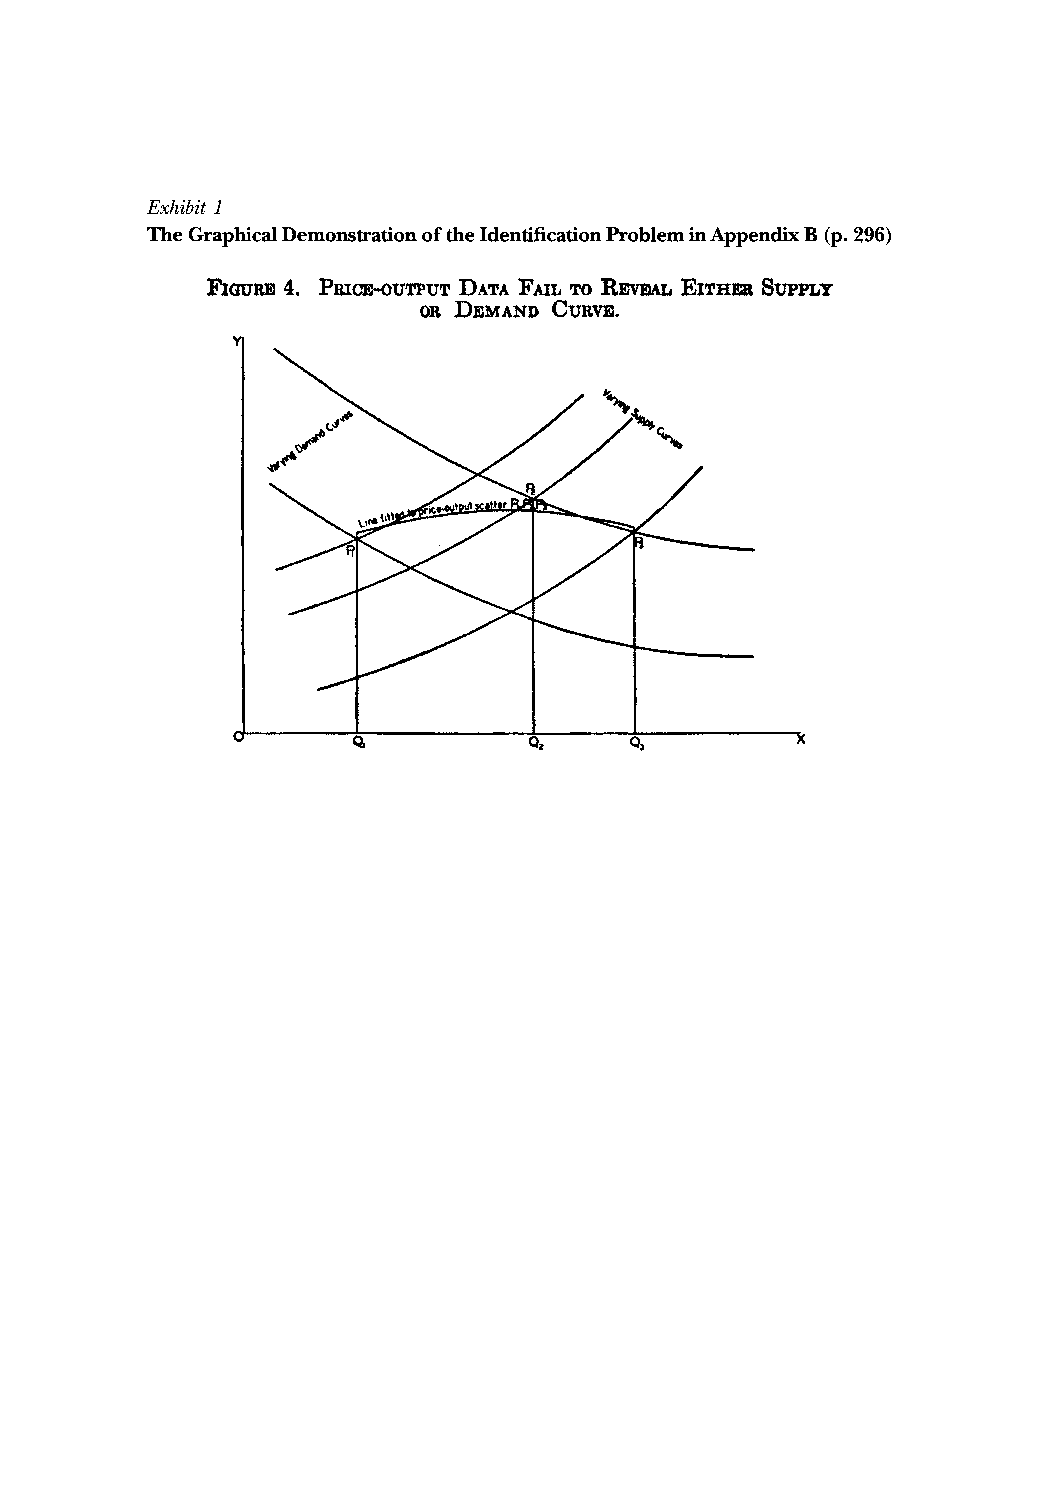
\includegraphics[scale=0.72]{./lecture_includes/supply_demand.pdf}
	\end{figure}
\end{frame}


\begin{frame}{Initial price and quantity}

	\begin{figure}
	\includegraphics[scale=0.15]{./lecture_includes/elasticity_1.jpg}
	\end{figure}
\end{frame}

\begin{frame}{Supply shift}

	\begin{figure}
	\includegraphics[scale=0.15]{./lecture_includes/elasticity_2.jpg}
	\end{figure}
\end{frame}


\begin{frame}{Price elasticity of demand}

\begin{eqnarray*}
\delta = \frac{Q_2 - Q_1}{P_2 - P_1}
\end{eqnarray*}

\bigskip

Can be estimated with log-log regressions:

\bigskip

\begin{eqnarray*}
Ln Q_{it} = \alpha + \delta Ln P_{it} + \psi_{it}
\end{eqnarray*}

\bigskip

But you need an instrument for price and it must be a supply shifter only


\end{frame}

\begin{frame}{Supply shift}

\begin{itemize}
\item \textbf{Supply shifters}: Firm input costs and technology are typical candidates
\item \textcolor{red}{Demand shifters}: Other consumer good prices, consumer income, availability of substitutes, expectations about the future
\item Good instruments must shift \textbf{only} supply -- \textcolor{red}{not demand}
\end{itemize}

\end{frame}

\begin{frame}{Elasticity of meth demand}

	\begin{figure}
	\includegraphics[scale=0.25]{./lecture_includes/he_1}
	\end{figure}
\end{frame}

\begin{frame}{Cooking meth}

\begin{itemize}
\item d-methamphetamine is a chemical product synthesized from either ephedrine or pseudoephedrine 
\item 1995, 1997 and 2003 there were several federal regulations that restricted access to these precursors as an effort combat meth epidemic
\item Undercover meth seizure data showed massive increases in real price of meth on the street in response
\end{itemize}

\end{frame}

\begin{frame}{Meth purity plummetted}

	\begin{figure}
	\includegraphics[scale=0.35]{./lecture_includes/he_2}
	\end{figure}
\end{frame}

\begin{frame}{Meth prices skyrocketed}

	\begin{figure}
	\includegraphics[scale=0.35]{./lecture_includes/he_3}
	\end{figure}
\end{frame}

\begin{frame}{Meth admissions to treatment and hospitals fell}

	\begin{figure}
	\includegraphics[scale=0.35]{./lecture_includes/he_4}
	\end{figure}
\end{frame}


\begin{frame}{OLS and 2SLS Estimation}

	\begin{figure}
	\includegraphics[scale=0.35]{./lecture_includes/he_7}
	\end{figure}
\end{frame}

\begin{frame}{Discussion}

\begin{itemize}
\item Highly inelastic (-0.21 to -0.26) and robust across two measures of meth consumption
\item Need data on prices and quantities, required FOIA requests to Drug Enforcement Agency and purchasing data on hospitalizations and treatment
\item But crucially needed something that would've raised firm costs through inputs that was not related to consumer demand (theory guided)
\item Instruments were deviations in the price from longterm trends
\end{itemize}

\end{frame}

\begin{frame}{Discussion}

\begin{itemize}
\item There are other ways to estimate demand, but this method is one that should immediately be exploited when supply shocks happen
\item Focus needs to be on inputs for which there are not instantly the ability to substitute
\item But can't be so correlated with broader demand shocks that you are back shifting supply and demand (e.g., COVID)
\end{itemize}

\end{frame}

\section{Conclusion}

\begin{frame}{Conclusion}

\begin{itemize}
\item ``With a long enough lever, I can move the world'' -- Archimedes
\item With a strong enough and strange enough instrument, you can identify the LATE even outside of the laboratory
\item Need to know what to look for so keep that DAG in mind all the time -- write it on the wall
\item But like selection on observables, we need plausible assumptions, properly measured data and appropriate estimators
\end{itemize}

\end{frame}


\end{document}



\subsection{Leniency design}


\begin{frame}{Comments on judge fixed effects}

\begin{itemize}
	\item Leave-one-out average propensity of the decision-maker, or some residualized instrument, is very common
	\item More often you'll see jackknife IV (JIVE) which drops observations while running regressions to improve finite sample bias
	\item The biggest threats aren't exclusion probably (though sometimes), but monotonicity
	\item Might judges be harsh in some situations (violent crimes) but lenient in others (female defendants, first time offenders)
\end{itemize}

\end{frame}

\begin{frame}{Tests for violations}

\begin{itemize}
\item New paper by Frandsen, Lefgren and Leslie (2019) proposes a test 
\item They show that the identifying assumptions imply a conditional expectation of the outcome of interest given the judge assignment is a continuous function of the judge propensity 
\item They propose a two-part test that generalizes the Sargan-Hansen over identification test and assesses whether treatment effects across judge propensities are possible 
\item Software available on Emily Leslie's website
\end{itemize}

\end{frame}

\begin{frame}{Multi-dimensional instrument}

\begin{itemize}
\item Peter Hull in a cautionary note notes that while combining judge fixed effects into a single propensity is numerically equivalent, it's still a series of dummies
\item Therefore it's very important to keep in mind the lessons we learned from weak instruments -- the more weak instruments you have when a parameter is overidentified, the larger the bias
\item It's ongoing at the moment to think about ways to improve instrument selection, but not settled
\item I encourage you to read Peter's note on his website and begin thinking about this yourself
\end{itemize}

\end{frame}


\begin{frame}{Discussion questions}

\begin{itemize}
\item When working on a judge fixed effects project, write down an IV DAG 
\item Whereas monotonicity cannot be visualized to my knowledge on a DAG, exclusion can -- so what does an exclusion violation mean in this context?
\item Use logic and conversations with those administering the program to answer the following -- what does monotonicity mean in this context and how might it be violated?  
\end{itemize}

\end{frame}


\begin{frame}{Empirical exercise}

\begin{itemize}

\item Let's estimate the effect of cash bail on defendant outcomes using 2SLS and JIVE
\item Excellent paper by Megan Stevenson
\item -\texttt{bail.do}- and -\texttt{bail.r}- in dropbox and github
\end{itemize}

\end{frame}





\begin{frame}{Phillip Wright}
	
	\begin{itemize}
	\item Philip Wright was a renaissance man - published in JASA, QJE, AER, you name it, while on a very intense teaching load. 
	\item Also published poetry, and even personally published Carl Sandburg's first book of poetry!
	\item Spent a long time at Tufts
	\item He was very concerned about the negative effects of tariffs and wrote a book about commodity markets
	\end{itemize}

\end{frame}

\begin{frame}{Elasticity of demand is unidentified}
	
	\begin{itemize}
	\item James Stock notes that his publications had a theme regarding identification
	\item He knew, for instance, that he couldn't simple look at correlations between price and quantity if he wanted the elasticity of demand due to simultaneous shifts in supply and demand
	\item The pairs of quantity and price weren't demand, or supply - they were demand and supply equilibrium values and therefore didn't reflect the demand or the supply curve, both of which are counterfactuals
	\item Those points are nothing more than a bunch of numbers -- no more, no less -- that have no practical use, scientific or otherwise
	\end{itemize}
	
\end{frame}

\begin{frame}[plain]

 \begin{figure}[h]
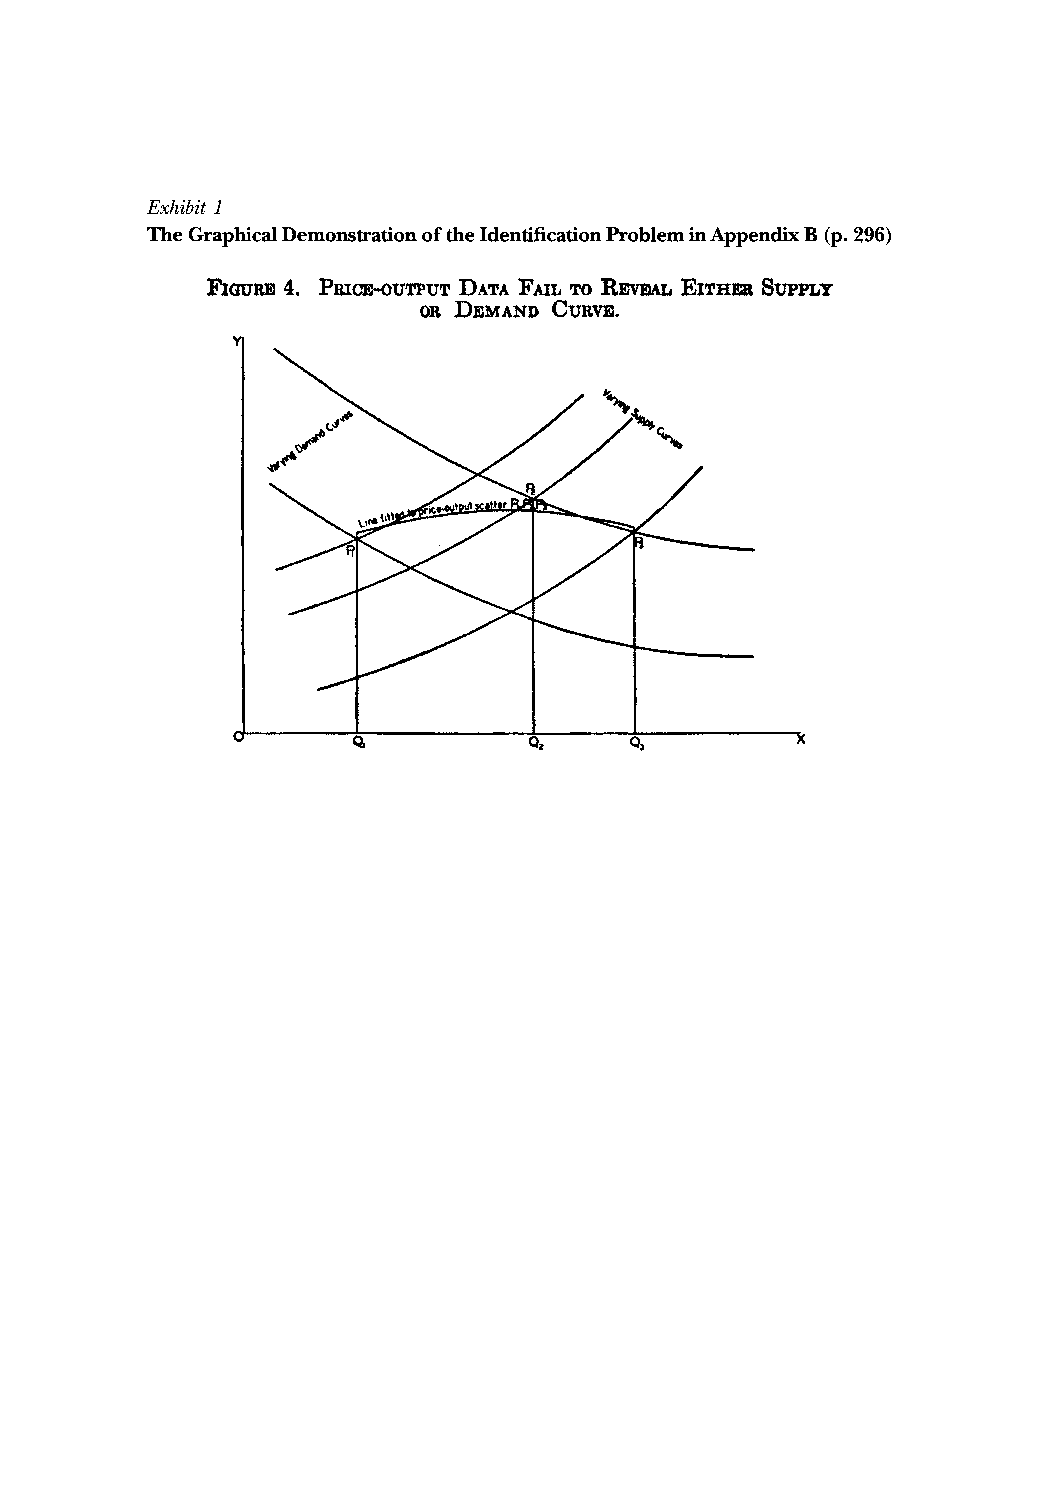
\includegraphics[scale=0.75]{./lecture_includes/supply_demand.pdf}
\caption{Wright's graphical demonstration of the identification problem}
\label{fig:sd}
\end{figure}

\end{frame}

\begin{frame}{Sewell Wright}

\begin{itemize}
\item Sewell was his son, who did \emph{not} go into the family business
\item Rather, he decided to become a genius and invent genetics
\item Developed path diagrams (which Pearl revived 50 years later for causal inference) 
\item Father and son engage in letter correspondence as Philip tried to solve the ``identification problem''

\end{itemize}

\end{frame}

\begin{frame}[plain]


\centering
  \begin{overprint}%
\begin{figure}[h]
  \makebox[\textwidth][c]{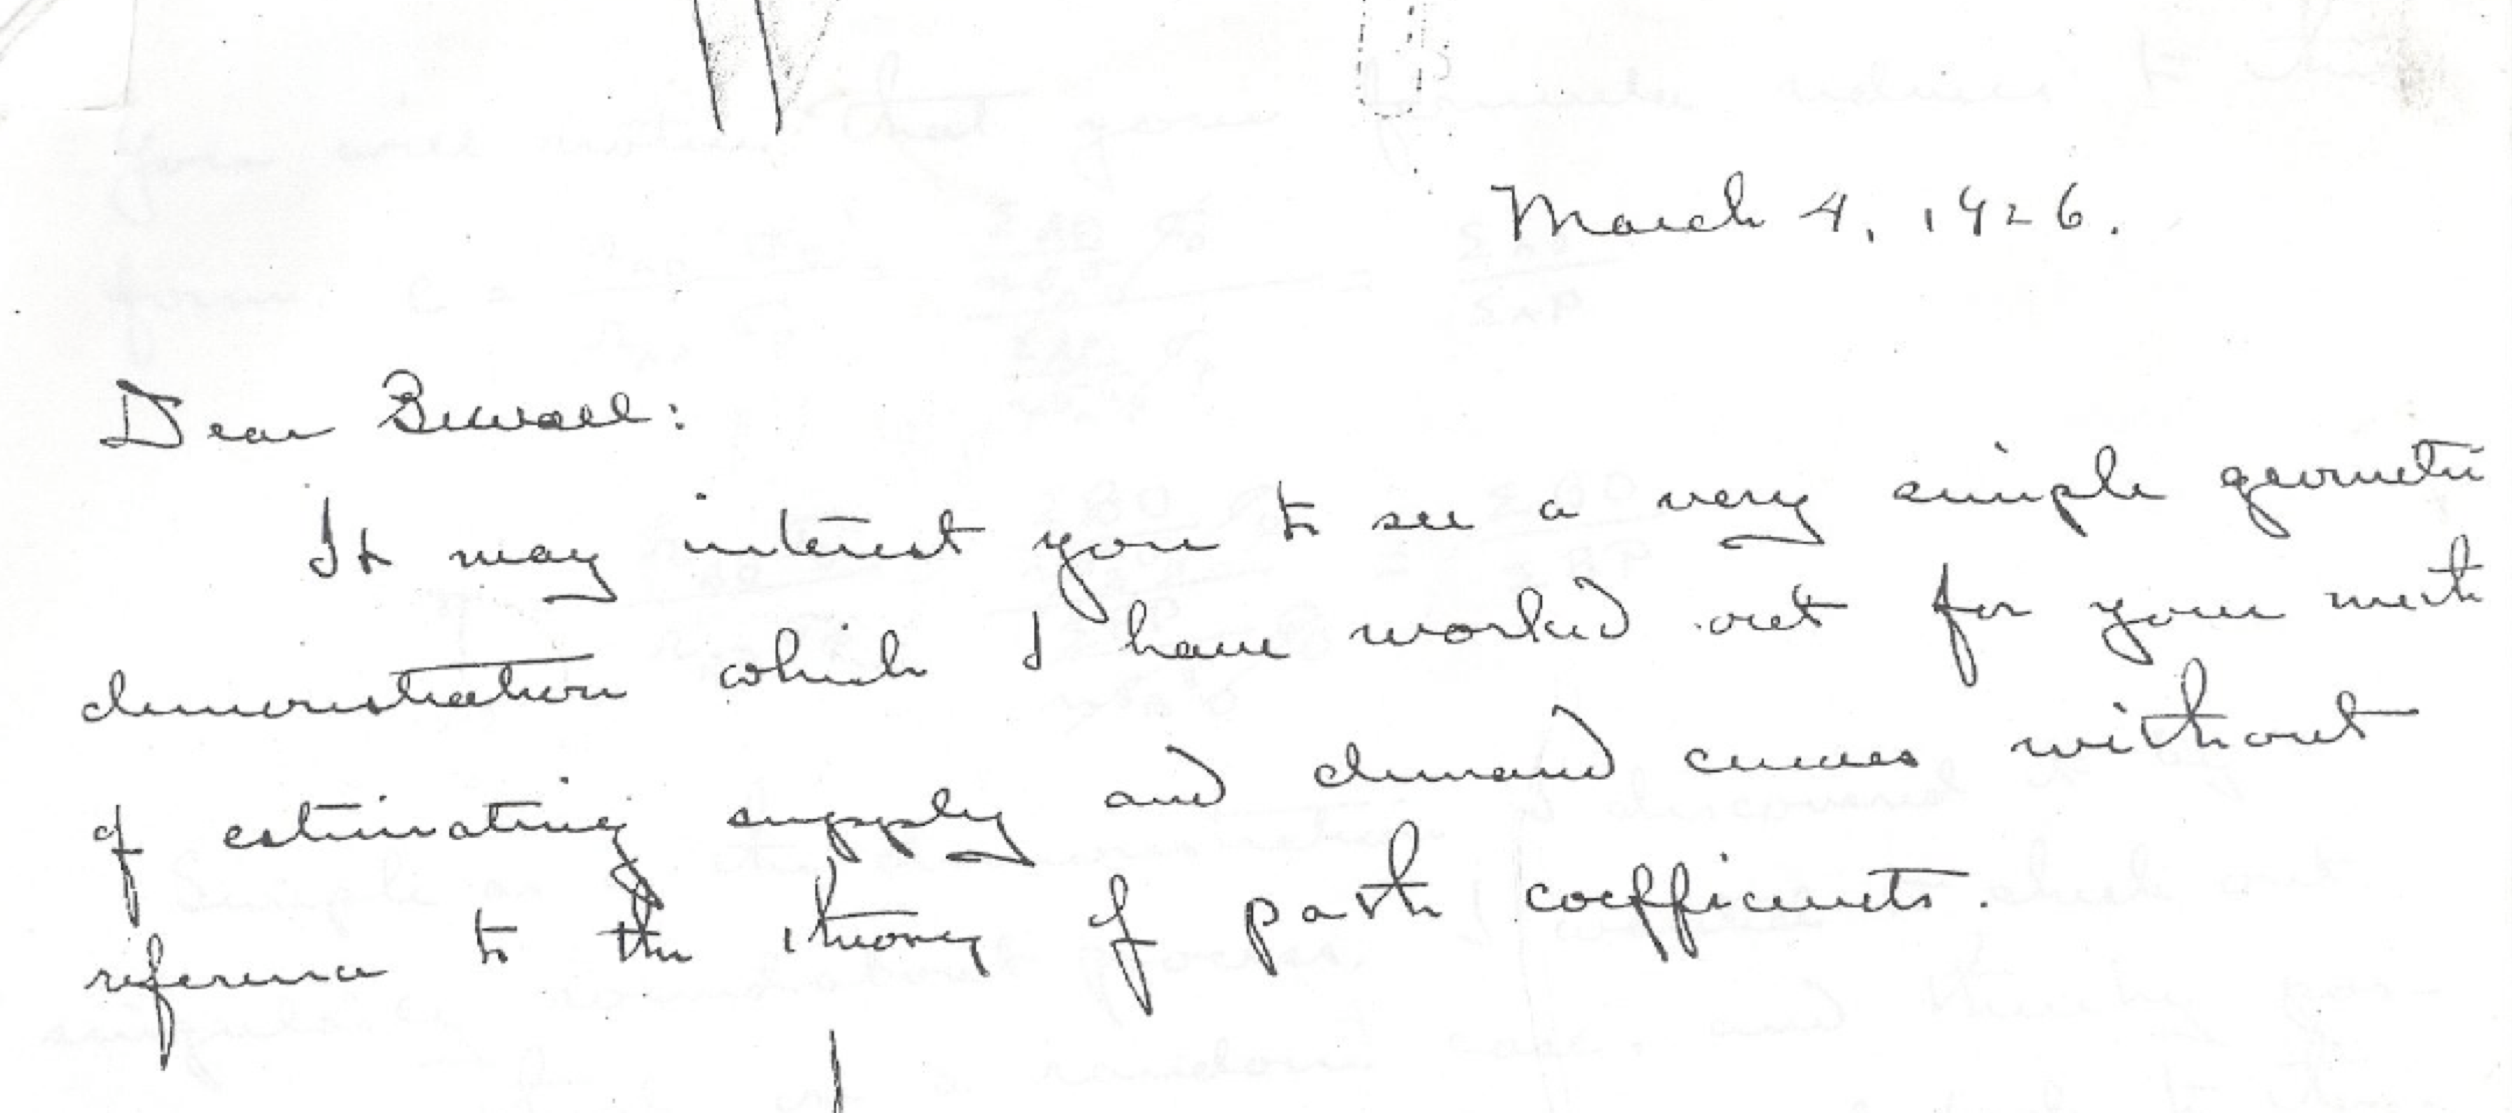
\includegraphics[width=1.0\textwidth]{./lecture_includes/wright_letter.png}}%
\caption{Wright's letter to Sewell, his son}
\end{figure}
  \end{overprint}%

\end{frame}


\begin{frame}[plain]


\centering
  \begin{overprint}%
\begin{figure}[h]
  \makebox[\textwidth][c]{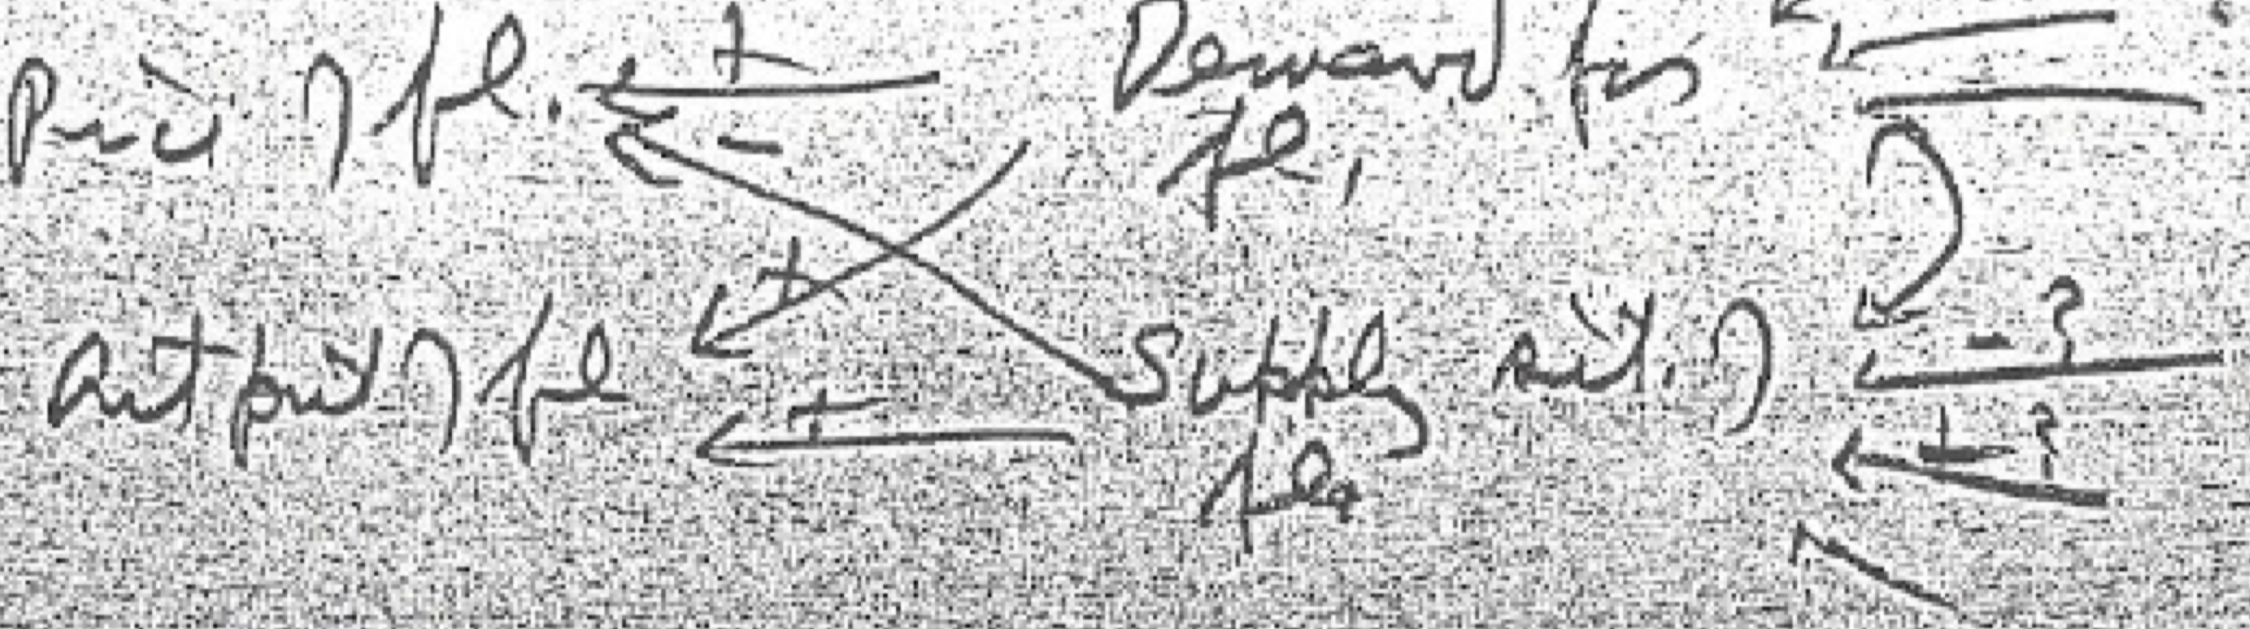
\includegraphics[width=1.0\textwidth]{./lecture_includes/path_diagrams_wrights.png}}%
\caption{Recognize these?}
\end{figure}
  \end{overprint}%

\end{frame}


\begin{frame}{QJE Rejects}

\begin{itemize}
\item QJE misses a chance to make history and rejects his paper proving an IV estimator
\item Sticks his proof in Appendix B of 1928 book, \underline{The Tariff on Animal and Vegetable Oils}
\item His work on IV is ignored, and is then rediscovered 15 years later (e.g., Olav Reiers\o l). 
\item James Stock and others have helped correct the record
\end{itemize}

\end{frame}


\begin{frame}{Sidebar: stylometric analysis}

\begin{itemize}
\item Long standing question was who \emph{wrote} Appendix B? Answer according to Stock and Trebbi (2003) using stylometric methods is that Philip \emph{wrote} it.
\item But who invented it?  It was collaborative, but Sewell acknowledged he didn't know how to handle endogeneity and simultaneity (that was Philip)
\end{itemize}

\end{frame}


\subsection{Lottery designs}


\begin{frame}{IV in Randomized Trials}
	
	\begin{itemize}
	\item In many randomized trials, participation is nonetheless voluntary among those randomly assigned to treatment
	\item Consequently, noncompliance is not uncommon and without correcting for it, creates selection biases
	\item IV designs may even be helpful when evaluating a randomized trial, even though treatment was randomly assigned
	\item The solution is to instrument for treatment with whether you ``won the lottery'' and estimate LATE
	\end{itemize}
	
\end{frame}

	
\begin{frame}{Lottery designs}
	
	\begin{itemize}
	\item The instrument is your randomized lottery
	\item Examples might be randomized lottery for attending charter schools to study effect of charter schools on educational outcomes, or a randomized voucher to encourage the collection of health information
	\item Recall Thornton (2008) instrumented for getting HIV results to estimate causal effect of learning one was HIV+ on condom purchases
	\item We'll discuss two papers from 2012 and 2014 evaluating a lottery-based expansion of Medicaid health insurance on Oregon on numerous health and financial outcomes
	\end{itemize}
\end{frame}


\begin{frame}{Overarching question}
	
	\begin{itemize}
	\item What are the effects of expanding access to public health insurance for low income adults?
		\begin{itemize}
		\item Magnitudes, and even the signs, associated with that question were uncertain
		\end{itemize}
	\item Limited existing evidence
		\begin{itemize}
		\item Institute of Medicine review of evidence was suggestive, but a lot of uncertainty
		\item Observational studies are confounded by selection into health insurance
		\item Quasi-experimental work often focuses on elderly and children
		\item Only one randomized experiment in a developed country: the RAND health insurance experiment
			\begin{itemize}
			\item 1970s experiment on a general population
			\item Randomized cost-sharing, not coverage itself
			\end{itemize}
		\end{itemize}
	\end{itemize}
\end{frame}



\begin{frame}{The Oregon Health Insurance Experiment}
	
	 Setting: Oregon Health Plan Standard
		\begin{itemize}
		\item Oregon's Medicaid expansion program for poor adults
		\item Eligibility
			\begin{itemize}
			\item Poor ($<$100\% federal poverty line) adults 19-64
			\item Not eligible for other programs
			\item Uninsured $>$ 6 months
			\item Legal residents
			\end{itemize}
		\item Comprehensive coverage (no dental or vision)
		\item Minimum cost-sharing
		\item Similar to other states in payments, management 
		\item Closed to new enrollment in 2004
		\end{itemize}
\end{frame}



\begin{frame}{The Oregon Medicaid Experiment}
	
Oregon held a lottery
		\begin{itemize}
		\item Waiver to operate lottery
		\item 5-week sign-up period, heavy advertising (January to February 2008)
		\item Low barriers to sign up, no eligibility pre-screening
		\item Limited information on list
		\item Randomly drew 30,000 out of 85,000 on list (March-October 2008)
		\item Those selected given chance to apply
			\begin{itemize}
			\item Treatment at household level
			\item Had to return application within 45 days
			\item 60\% applied; 50\% of those deemed eligible $\rightarrow$ 10,000 enrollees 
			\end{itemize}
		\end{itemize}
\end{frame}

\begin{frame}{Oregon Health Insurance Experiment}
	
	\begin{itemize}
	\item Evaluate effects of Medicaid using lottery as randomized controlled trial (RCT)
		\begin{itemize}
		\item Intent-to-treat: Reduced form comparison of outcomes between treatment group (lottery selected individuals) and controls (not selected)
		\item LATE: IV using lottery as instrument for insurance coverage
			\begin{itemize}
			\item First stage: about a 25 percentage point increase in insurance coverage
			\end{itemize}
		\item Archived analysis plan
		\item Massive data collect effort -- primary and secondary
		\end{itemize}
	\item Similar to ACA expansion but limits to generalizability
		\begin{itemize}
		\item Partial equilibrium vs. General equilibrium
		\item Mandate and external validity
		\item Oregon vs. other states
		\item Short vs. Long-run
		\end{itemize}
	\end{itemize}
\end{frame}
		

\begin{frame}{Examine Broad Range of Outcomes}
	
	\begin{itemize}
	\item Costs: Health care utilization
		\begin{itemize}
		\item Insurance increases resources (income) and lowers price, increasing utilization
		\item But improved efficiency (and improved health), decreasing utilization (``offset'')
		\item Additional uncertainty when comparing Medicaid to no insurance
		\end{itemize}
	\item Benefits I: Financial risk exposure
		\begin{itemize}
		\item Insurance supposed to smooth consumption
		\item But for very low income, is most care \emph{de jure} or \emph{de facto} free?
		\end{itemize}
	\item Benefits II: Health
		\begin{itemize}
		\item Expected to improve (via increased quantity / quality of care)
		\item But could discourage health investments (``\emph{ex ante} moral hazard'')
		\end{itemize}
	\end{itemize}
\end{frame}

\begin{frame}{Data}
	
	\begin{itemize}
	\item Pre-randomization demographic information
		\begin{itemize}
		\item From lottery sign-up
		\end{itemize}
	\item State administrative records on Medicaid enrollment
		\begin{itemize}
		\item Primary measure of first stage (i.e., insurance coverage)
		\end{itemize}
	\item Outcomes
		\begin{itemize}
		\item Administrative data ($\sim$16 months post-notification): Hospital discharge data, mortality, credit reports
		\item Mail surveys ($\sim$15 months): some questions ask 6-month look-back; some ask current
		\item In-person survey and measurements ($\sim$25 months): Detailed questionnaires, blood samples, blood pressure, body mass index
		\end{itemize}
	\end{itemize}
\end{frame}

\imageframe{./lecture_includes/baicker_1.pdf}

\begin{frame}{Empirical Framework}
	
	\begin{itemize}
	\item They present reduced form estimates of the causal effect of lottery selection$$Y_{ihj} = \beta_0 + \beta_1LOTTERY_{h} + X_{ih}\beta_2+V_{ih}\beta_3 + \varepsilon_{ihj}$$
	\item Validity of experimental design: randomization; balance on treatment and control. This is what readers expect
	\end{itemize}
\end{frame}


\begin{frame}{Empirical framework}

\begin{itemize}
	\item They also present IV results because they want to isolate the causal effect of insurance coverage
		\begin{eqnarray*}
		INSURANCE_{ihj} &=& \delta_0 + \delta_1LOTTERY_{ih} + X_{ih}\delta_2 + V_{ih}\delta_3 + \mu_{ihj} \\
		y_{ihj} &=& \pi_0 + \pi_1 \widehat{INSURANCE}_{ih} + X_{ih}\pi_2 + V_{ih}\pi_3 + v_{ihj}
		\end{eqnarray*}
		\item Effect of lottery on coverage: about 25 percentage points
		\item We have independence guaranteed; now we need exclusion: the primary pathway of the lottery must be via being on Medicaid
			\begin{itemize}
			\item Could affect participation in other programs, but actually small
			\item ``Warm glow'' of winning -- especially early
			\end{itemize}
	\item Analysis plan, multiple inference adjustment
\end{itemize}
\end{frame}

\begin{frame}{Effect of lottery on coverage (first stage)}
	
	\begin{figure}
	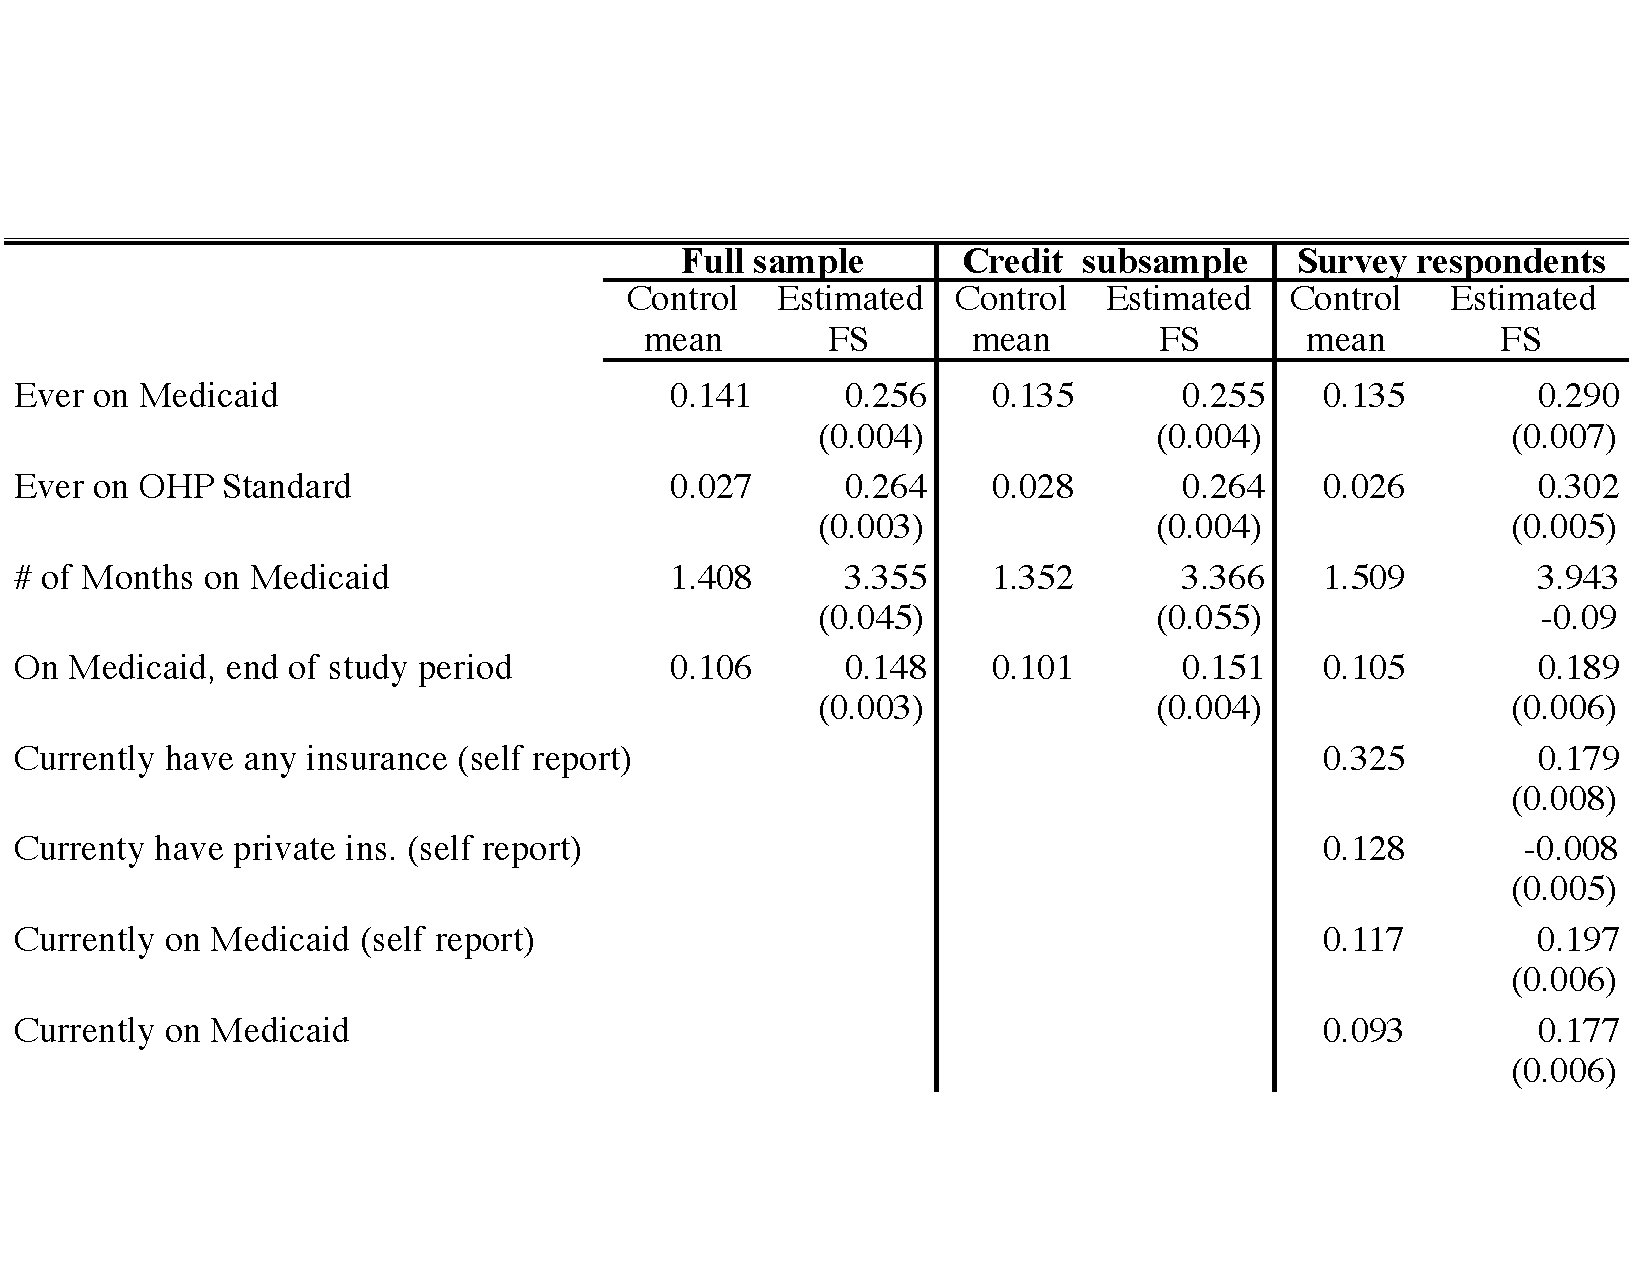
\includegraphics[scale=0.35]{./lecture_includes/baicker_2.pdf}
	\end{figure}
\end{frame}


\begin{frame}{Amy Finkelstein, et al. (2012). ``The Oregon Health Insurance Experiment: Evidence from the First Year'', \emph{Quarterly Journal of Economics}, vol. 127, issue 3, August. }
\end{frame}

\begin{frame}{Effects of Medicaid}
	
 Use primary and secondary data to gauge 1-year effects
		\begin{itemize}
		\item Mail surveys: 70,000 surveys at baseline, 12 months
		\item Administrative data
			\begin{itemize}
			\item Medicaid enrollment records
			\item Statewide Hospital discharge data, 2007-2010
			\item Credit report data, 2007-2010
			\item Mortality data, 2007-2010
			\end{itemize}
		\end{itemize}
\end{frame}

\begin{frame}{Mail survey data}
	
	\begin{itemize}
	\item \textbf{Fielding protocol}
		\begin{itemize}
		\item $\sim$70,000 people, surveyed at baseline and 12 months later
		\item Basic protocol: three-stage male survey protocol, English/Spanish
		\item Intensive protocol on a 30\% subsample included additional tracking, mailings, phone attempts (done to adjust for non-response bias)
		\end{itemize}
	\item \textbf{Response rate}
		\begin{itemize}
		\item Effective response rate = 50\%
		\item Non-response bias aways possible, but response rate and pre-randomization measures in administrative data were balanced between treatment and control
		\end{itemize}
	\end{itemize}
\end{frame}

\begin{frame}{Administrative data}
	
	\begin{itemize}
	\item \textbf{Medicaid records}
		\begin{itemize}
		\item Pre-randomization demographics from list
		\item Enrollment records to assess ``first stage'' (how many of the selected got insurance coverage)
		\end{itemize}
	\item \textbf{Hospital discharge data}
		\begin{itemize}
		\item Probabilistically matched to list, de-identified at Oregon Health Plan 
		\item Includes dates and source of admissions, diagnoses, procedures, length of stay, hospital identifier
		\item Includes years before and after randomization
		\end{itemize}
	\item \textbf{Other data}
		\begin{itemize}
		\item Mortality data from Oregon death records
		\item Credit report data, probabilistically matched, de-identified
		\end{itemize}
	\end{itemize}
\end{frame}

\begin{frame}{Sample}
	
	\begin{itemize}
	\item 89,824 unique individuals on the waiting list
	\item Sample exclusions (based on pre-randomization data only)
		\begin{itemize}
		\item Ineligible for OHP Standard (out of state address, age, etc.)
		\item Individuals with institutional addresses on list
		\end{itemize}
	\item Final sample: 79,922 individuals out of 66,385 households
		\begin{itemize}
		\item 29,834 treated individuals (surveyed 29,589)
		\item 40,088 control individuals (surveyed 28,816)
		\end{itemize}
	\end{itemize}
\end{frame}


\begin{frame}{Sample characteristics}
	
	\begin{figure}
	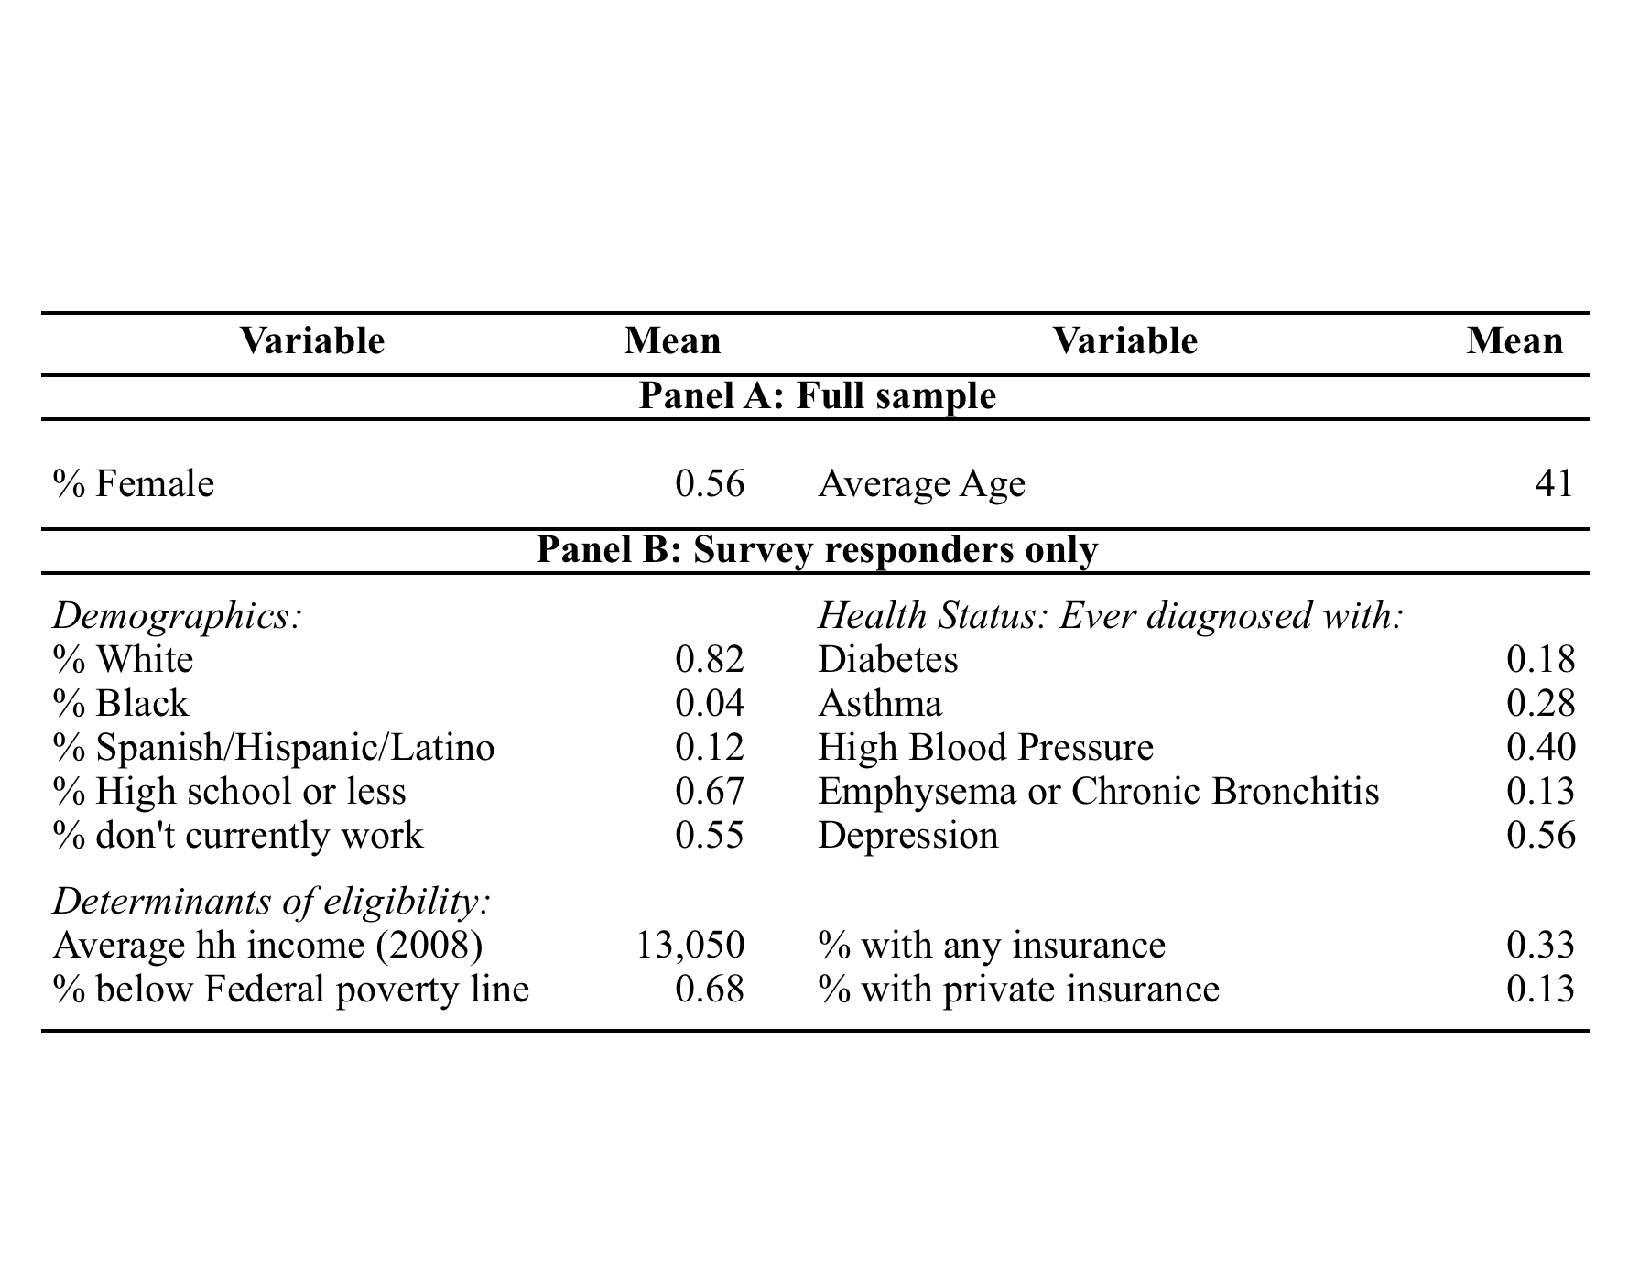
\includegraphics[scale=0.40]{./lecture_includes/baicker_3.pdf}
	\end{figure}
\end{frame}


\begin{frame}{Outcomes}
	
	\begin{itemize}
	\item \textbf{Access and use of care}
		\begin{itemize}
		\item Is access to care improved? Do the insured use more care? Is there a shift in the types of care being used?
		\item Mail surveys and hospital discharge data
		\end{itemize}
	\item \textbf{Financial strain}
		\begin{itemize}
		\item How much does insurance protect against financial strain?
		\item What are the out-of-pocket implications?
		\item Mail surveys and credit reports
		\end{itemize}
	\item \textbf{Health}
		\begin{itemize}
		\item What are the short-term impacts on self-reported physical and mental health?
		\item Mail surveys and vital statistics (mortality)
		\end{itemize}
	\end{itemize}
\end{frame}

\begin{frame}{Effect of lottery on coverage}

Gaining insurance resulted in better access to care and higher satisfaction with care (conditional on actually getting care)
		
	\begin{figure}
	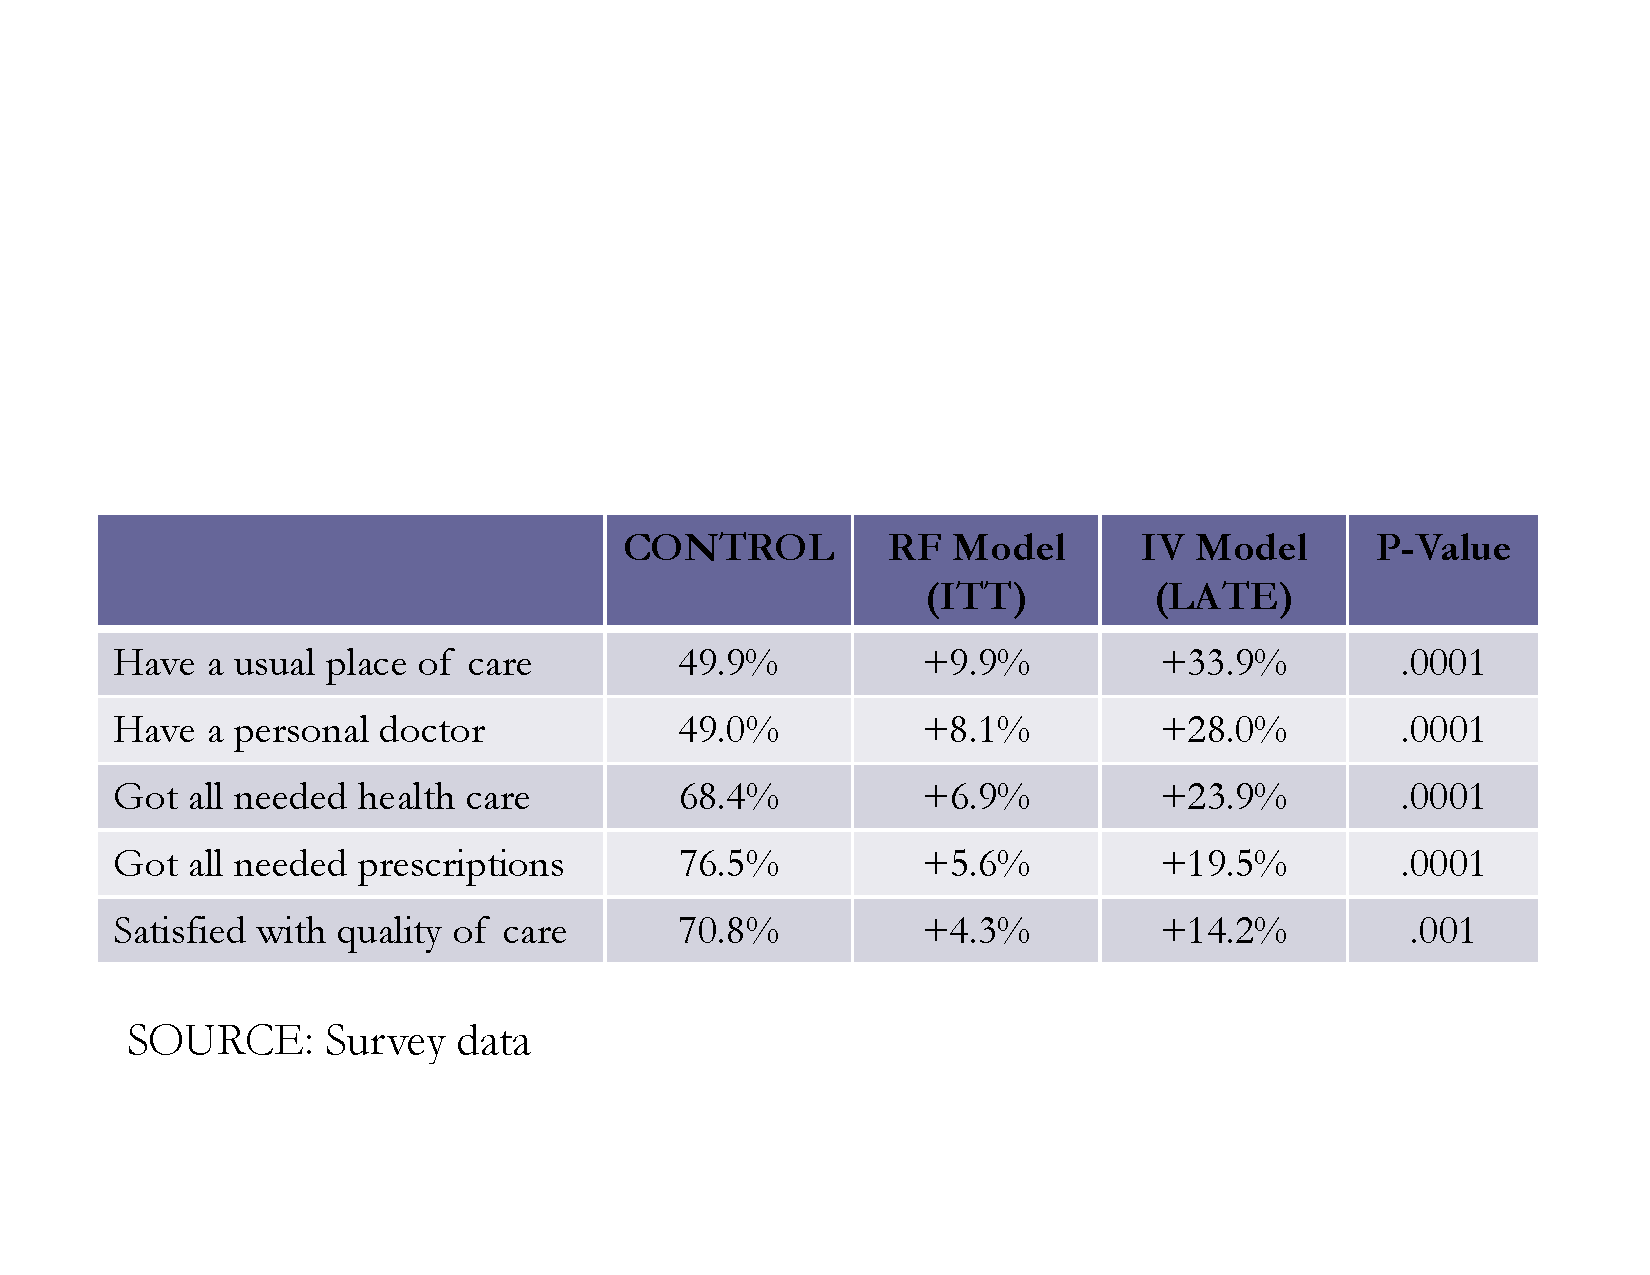
\includegraphics[scale=0.40]{./lecture_includes/baicker_4.pdf}
	\end{figure}
\end{frame}


\begin{frame}[plain]
	
	\begin{figure}
	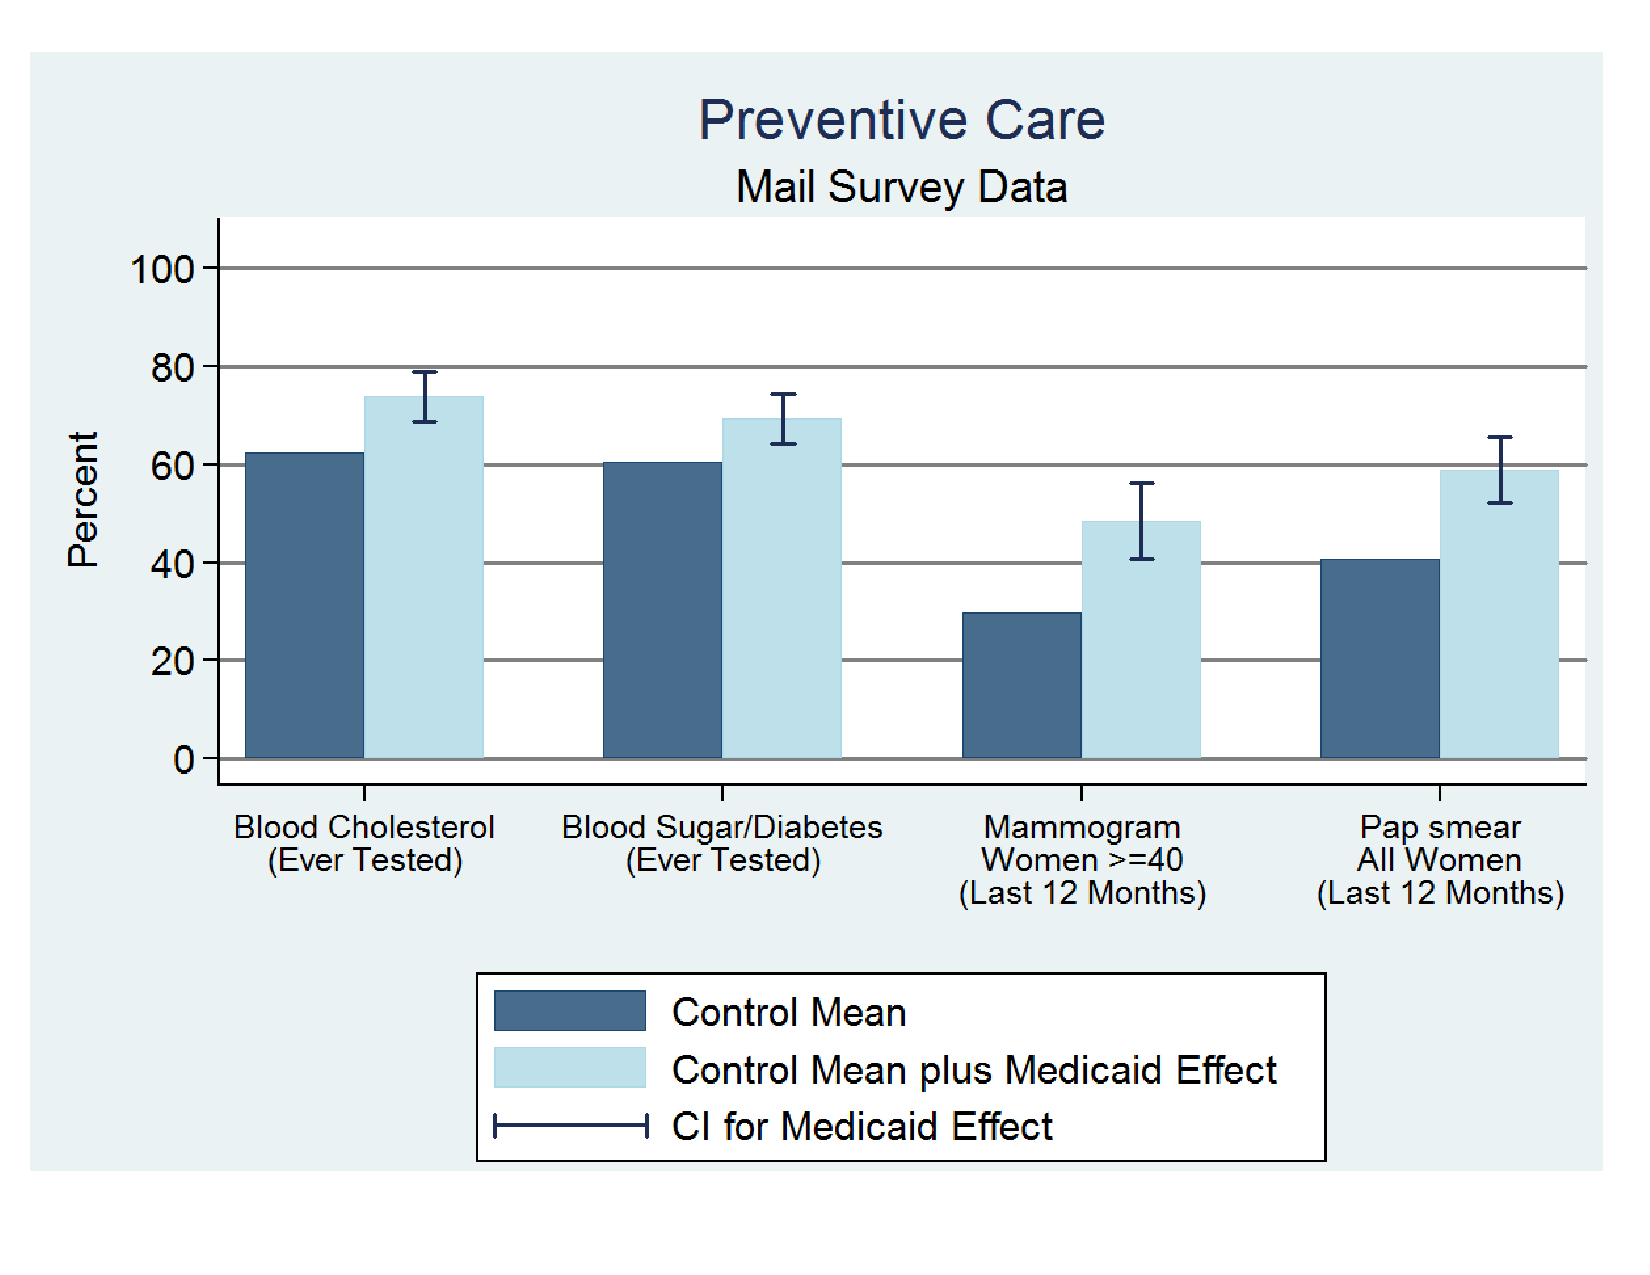
\includegraphics[scale=0.40]{./lecture_includes/baicker_5.pdf}
	\end{figure}
\end{frame}

\begin{frame}{Effect of lottery on coverage}

	 Gaining insurance resulted in increased probability of hospital admissions, primarily driven by non-emergency department admissions
		
	\begin{figure}
	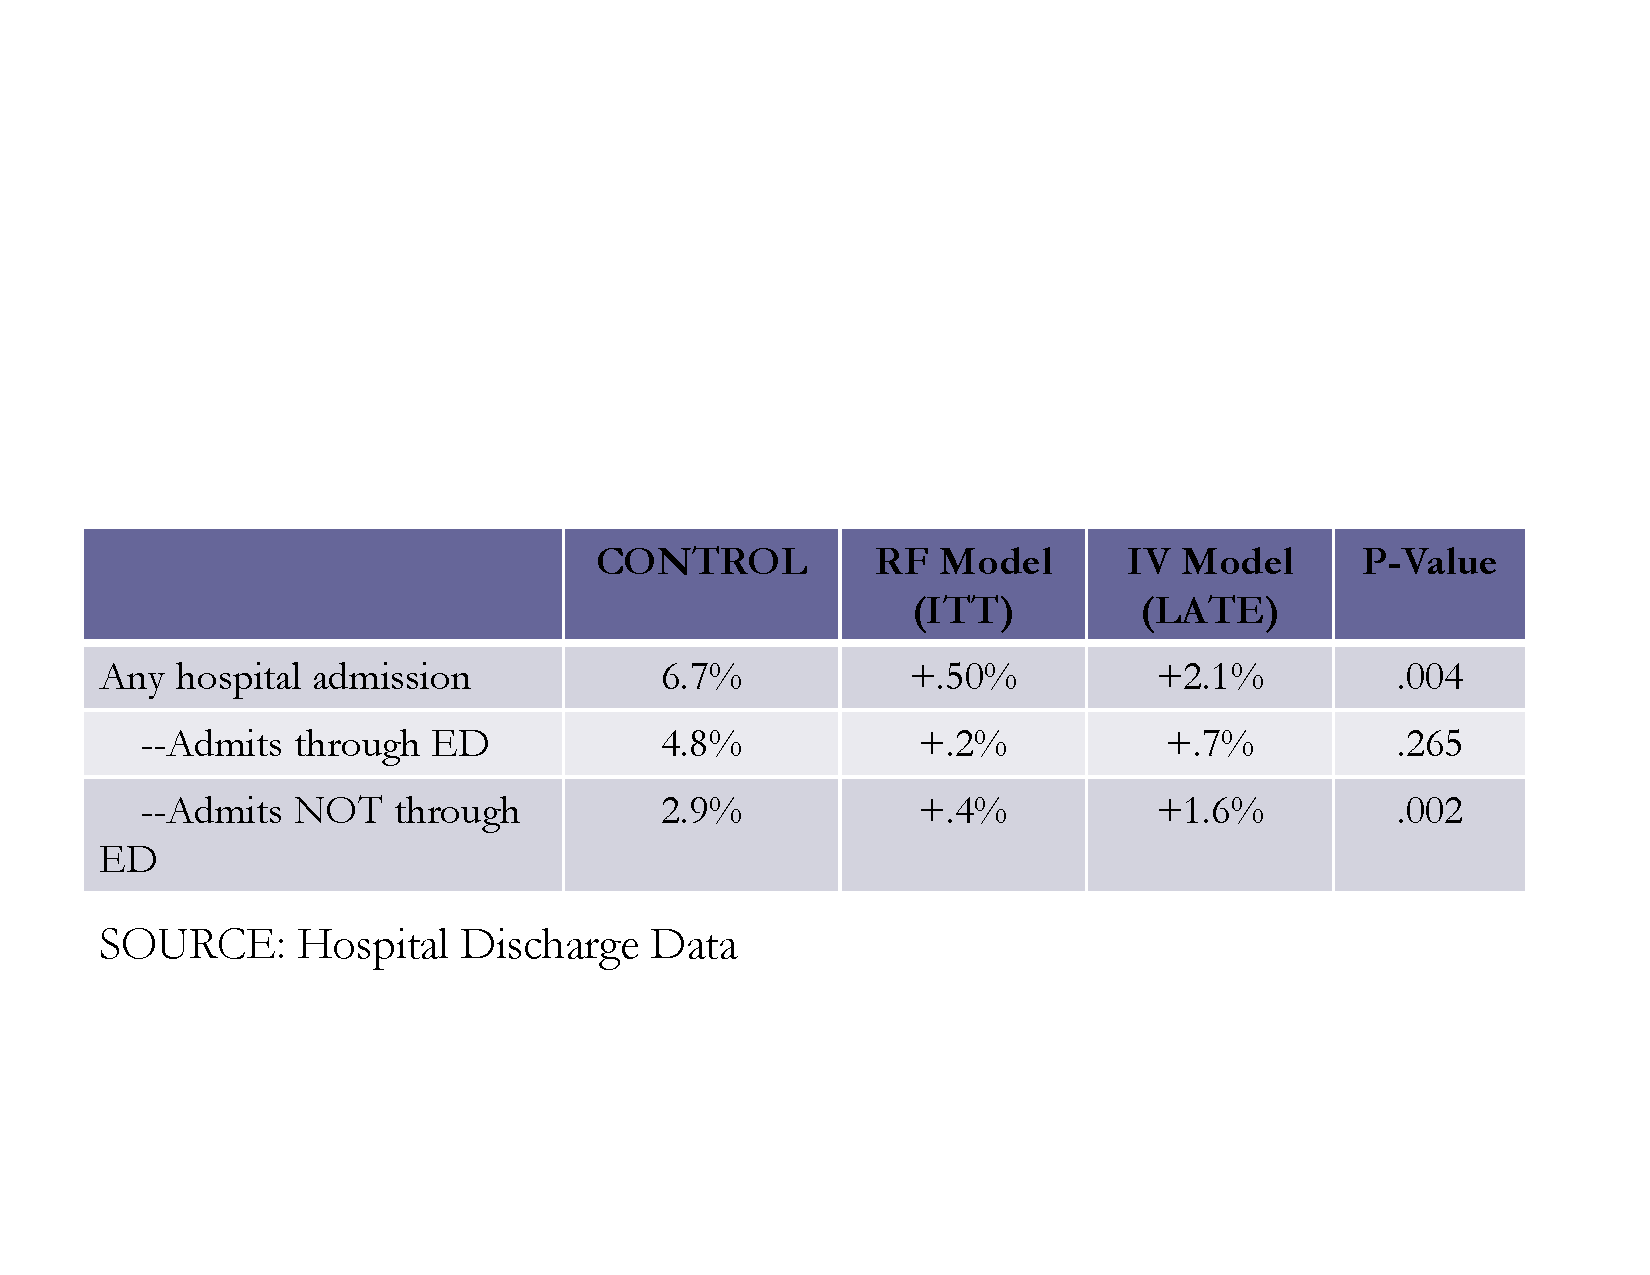
\includegraphics[scale=0.40]{./lecture_includes/baicker_6.pdf}
	\end{figure}
	
	Overall, this represents a 30\% higher probability of admission, although admissions are still rare events
\end{frame}

\begin{frame}[plain]
	
	\begin{figure}
	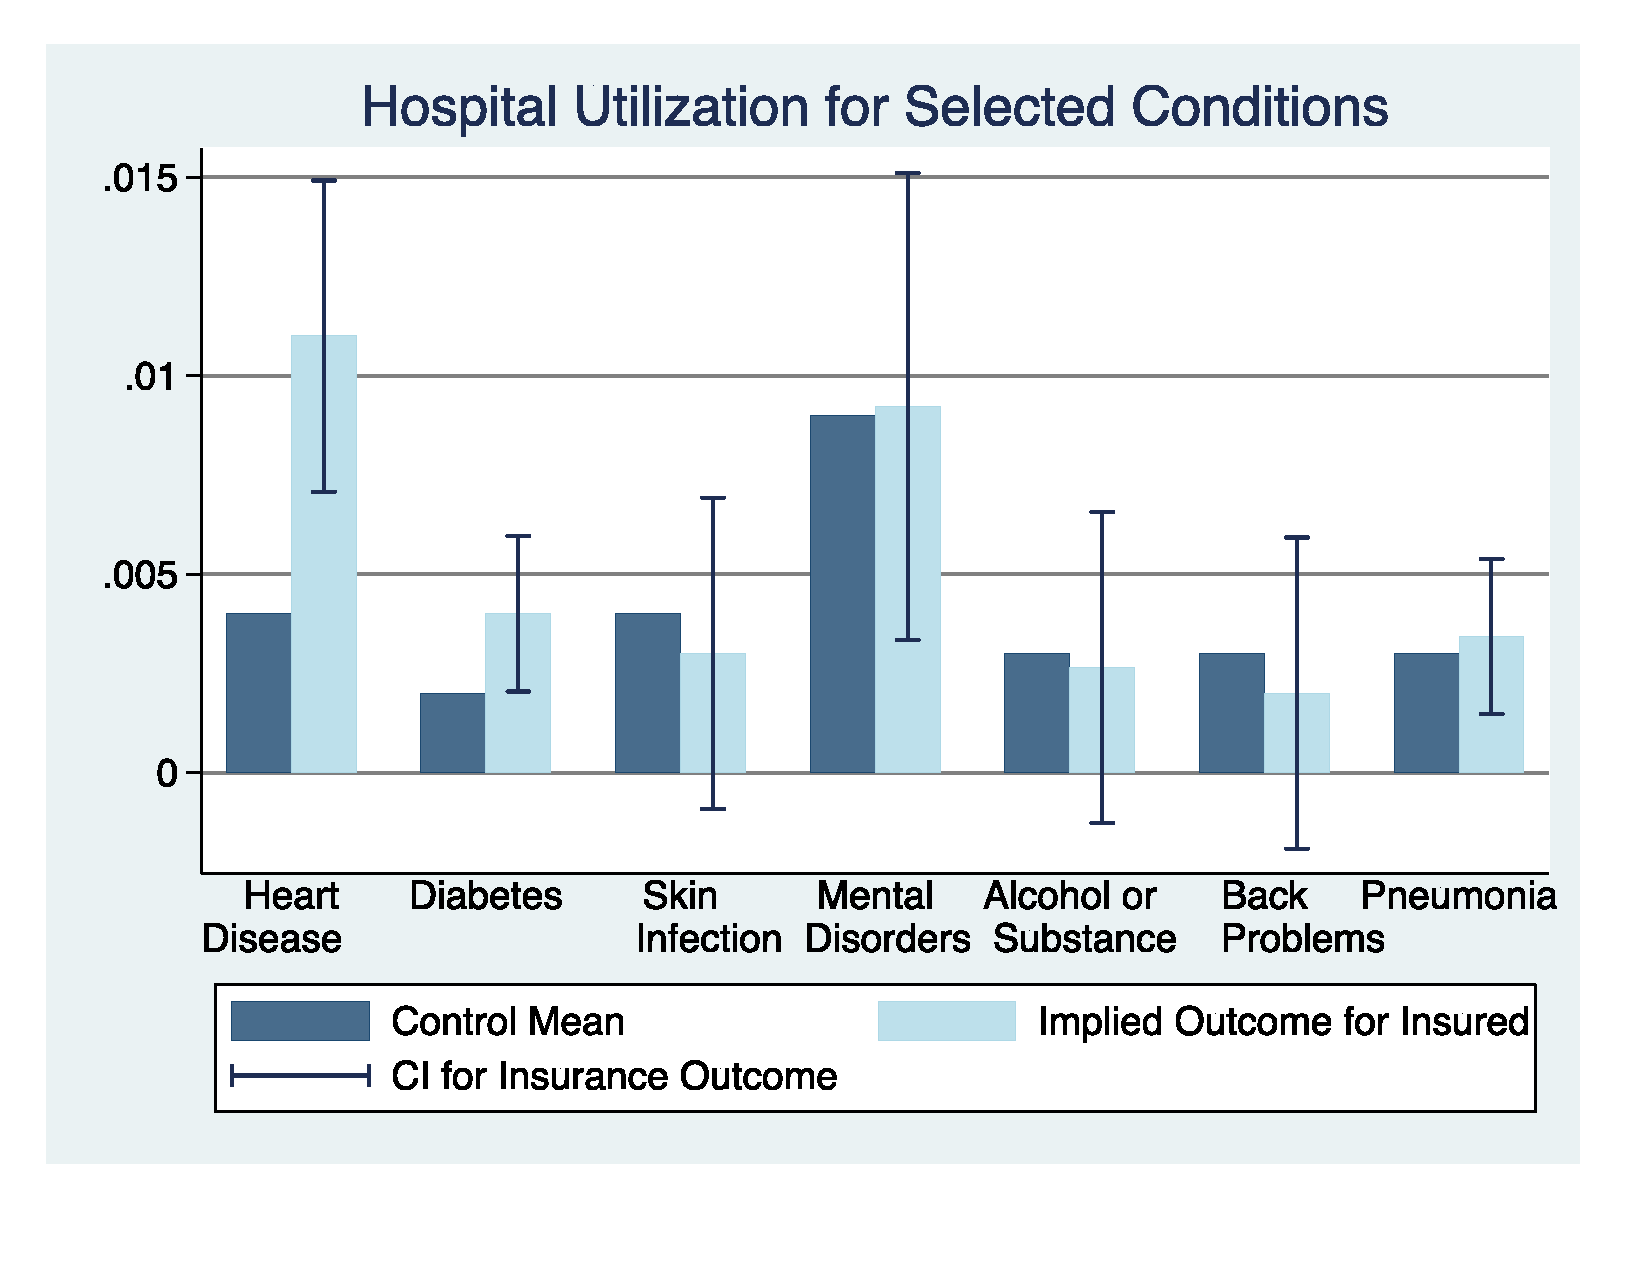
\includegraphics[scale=0.40]{./lecture_includes/baicker_7.pdf}
	\end{figure}
\end{frame}


\begin{frame}{Summary: Access and use of care}
	
	\begin{itemize}
	\item Overall, utilization and costs went up relative to controls
		\begin{itemize}
		\item 30\% increase in probability of an inpatient admission
		\item 35\% increase in probability of an outpatient visit
		\item 15\% increase in probability of taking prescription medications
		\item Total \$777 increase in average spending (a 25\% increase)
		\end{itemize}
	\item With this increased spending, those who gained insurance were
		\begin{itemize}
		\item 35\% more likely to get all needed care
		\item 25\% more likely to get all needed medications
		\item Far more likely to follow preventive care guidelines, such as mammograms (60\%) and PAP tests (45\%)
		\end{itemize}
	\end{itemize}
\end{frame}

\begin{frame}{Results: Financial Strain}

Gaining insurance resulted in a reduced probability of having medical collections in credit reports, and in lower amounts owed
		
	\begin{figure}
	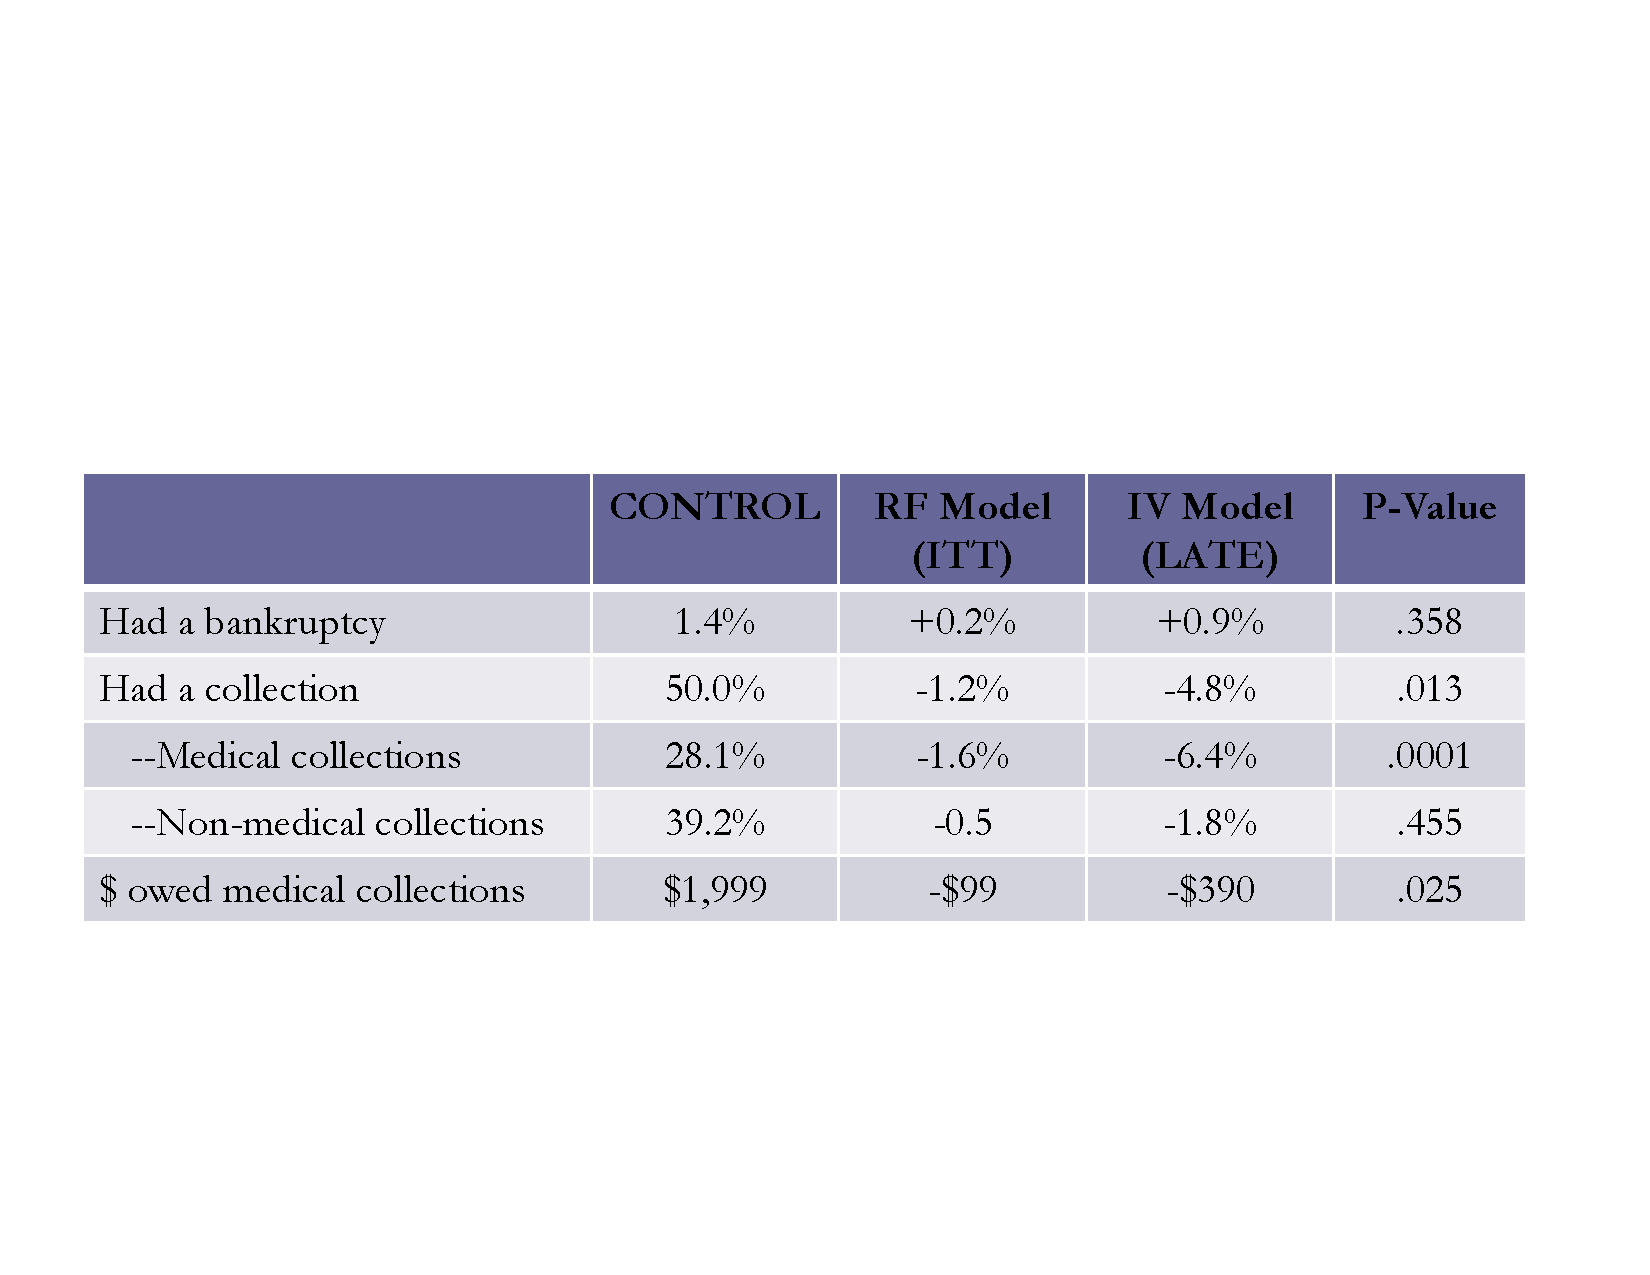
\includegraphics[scale=0.40]{./lecture_includes/baicker_8.pdf}
	\end{figure}
	
	Source: Credit report data
	
\end{frame}


\begin{frame}[plain]
	
	\begin{figure}
	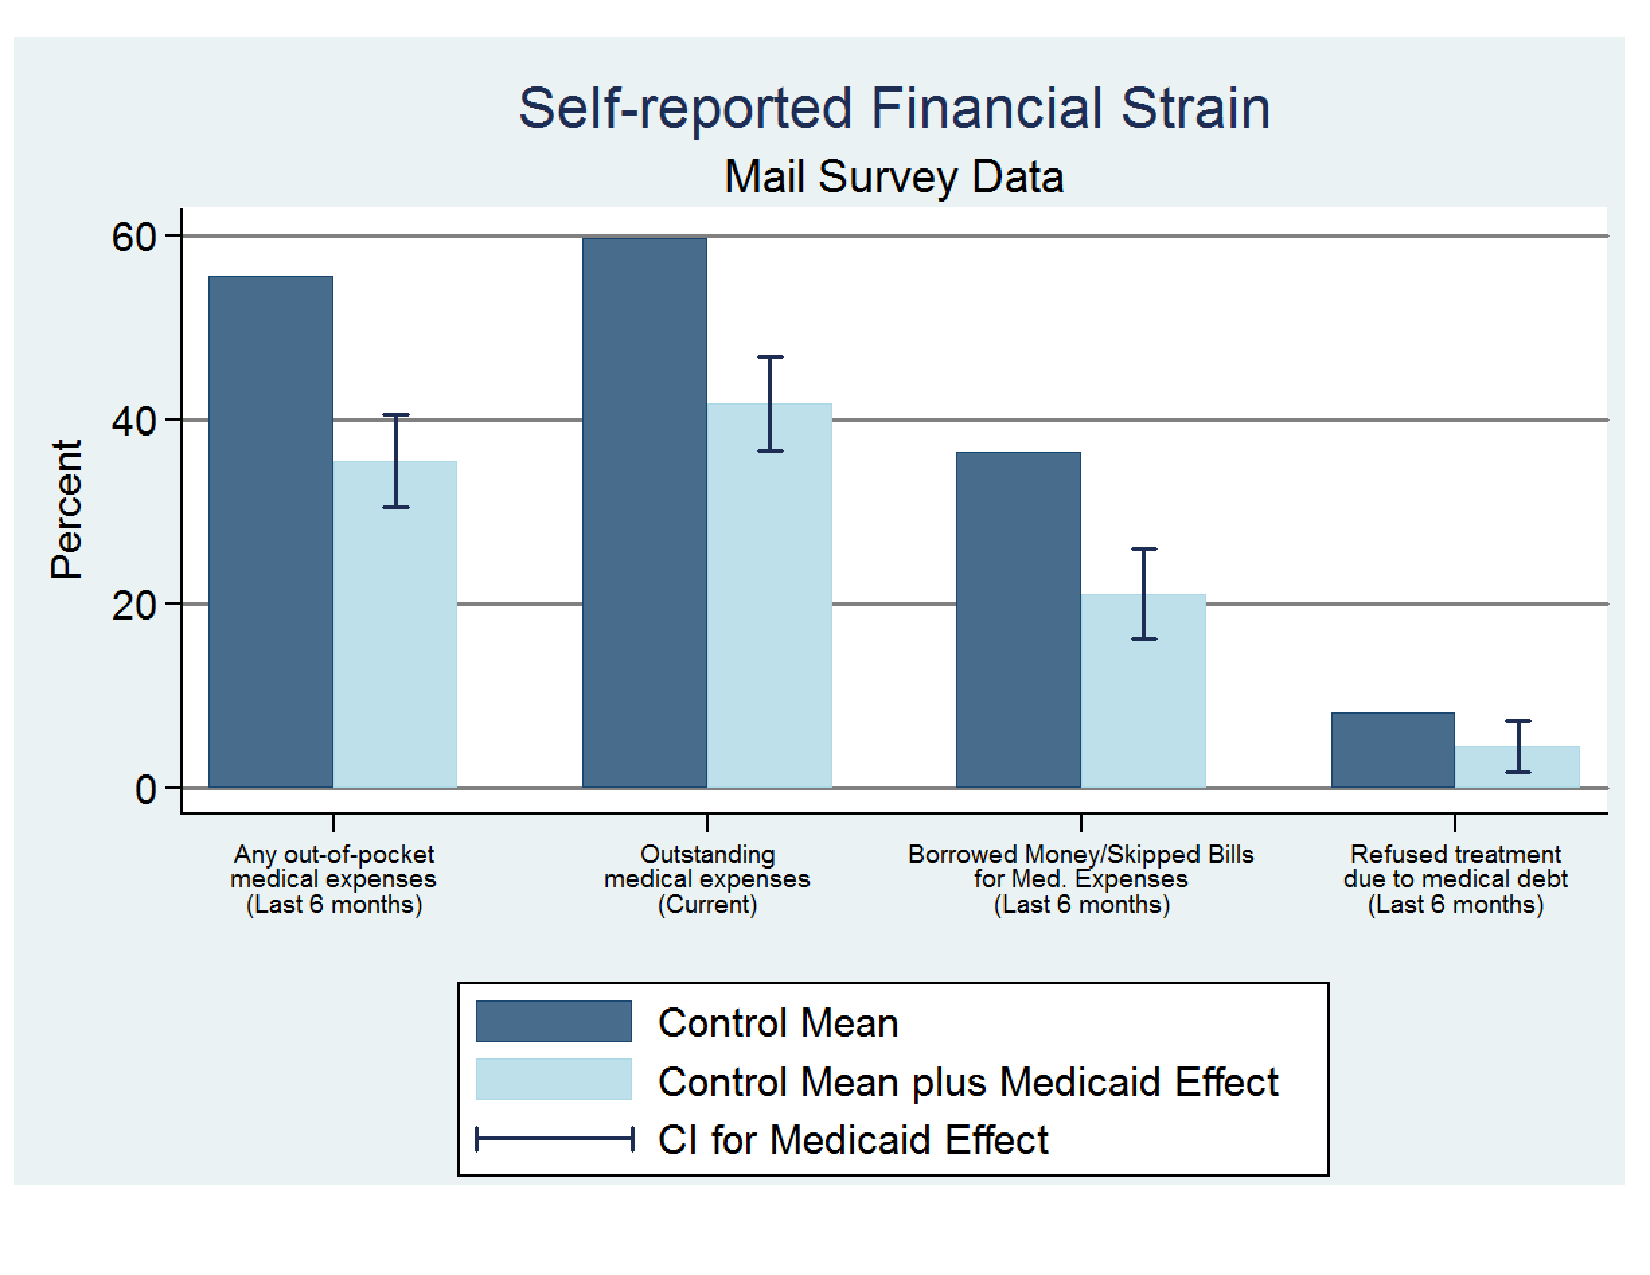
\includegraphics[scale=0.40]{./lecture_includes/baicker_9.pdf}
	\end{figure}
\end{frame}


\begin{frame}{Summary: Financial Strain}
	
	\begin{itemize}
	\item Overall, reductions in collections on credit reports were evident
		\begin{itemize}
		\item 25\% decrease in probability of a medical collection
		\item Those with a collection owed significantly less
		\end{itemize}
	\item Household financial strain related to medical costs was mitigated
		\begin{itemize}
		\item Substantial reduction across all financial strain measures
		\item Captures ``informal channels'' people use to make it work
		\end{itemize}
	\item Implications for both patients and providers
		\begin{itemize}
		\item Only 2\% of bills sent to collections are ever paid
		\end{itemize}
	\end{itemize}
\end{frame}



\begin{frame}{Results: Self-reported health}

Self-reported measures showed significant improvements one year after randomization
		
	\begin{figure}
	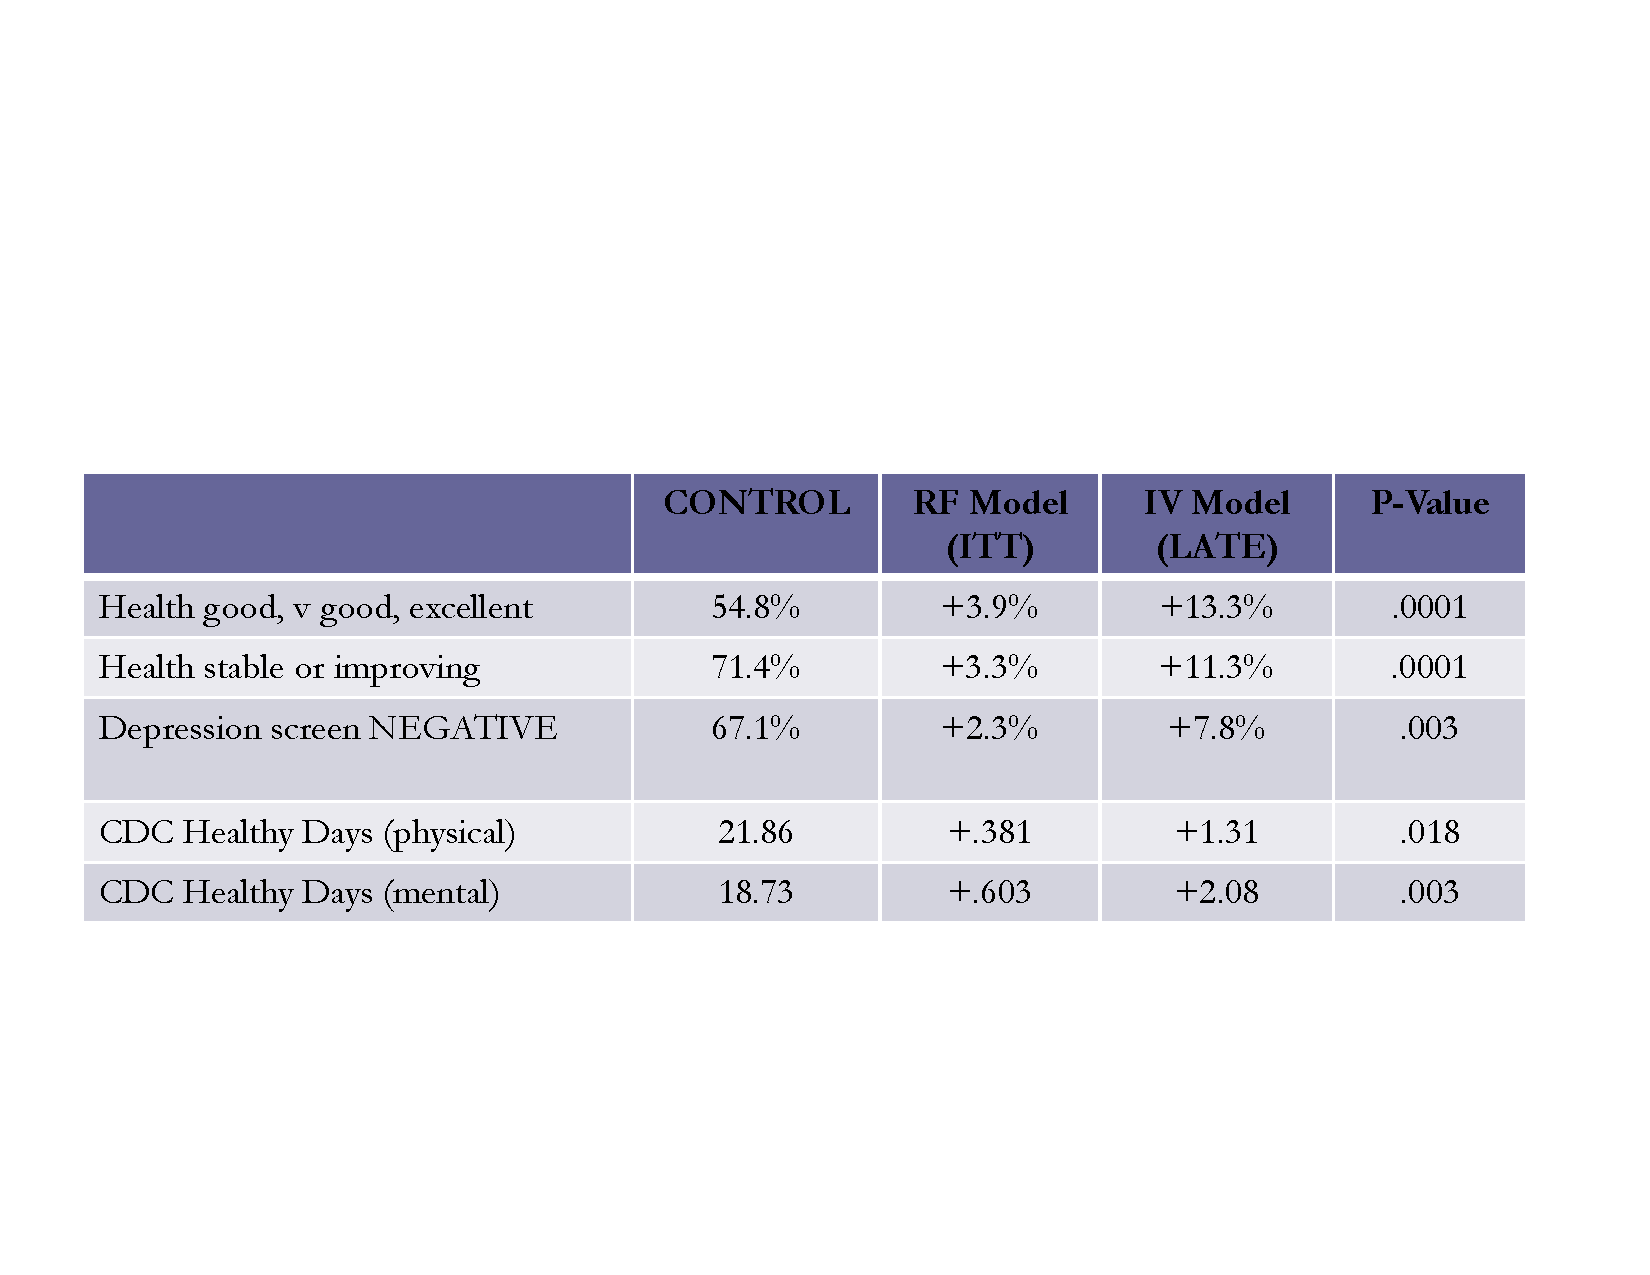
\includegraphics[scale=0.40]{./lecture_includes/baicker_10.pdf}
	\end{figure}
	
	Source: Survey data
	
\end{frame}



\begin{frame}{Summary: Self-reported health}
	
	\begin{itemize}
	\item Overall, big improvements in self-reported physical and mental health
		\begin{itemize}
		\item 25\% increase in probability of good, very good or excellent health
		\item 10\% decrease in probability of screening for depression
		\end{itemize}
	\item Physical health measures open to several interpretations
		\begin{itemize}
		\item Improvements consistent with findings of increased utilization, better access, and improved quality
		\item BUT in their baseline surveys, results appeared shortly after coverage ($\sim$2/3rds magnitude of full result)
		\item May suggest increase in \emph{perception} of well-being rather than physical health
		\end{itemize}
	\item Biomarker data can shed light on this issue
	\end{itemize}
\end{frame}

\begin{frame}{Discussion}
	
	\begin{itemize}
	\item At 1 year, found increases in utilization, reductions in financial strain, and improvements in self-reported health	
		\begin{itemize}
		\item Medicaid expansion had benefits and costs -- didn't ``pay for itself''
		\item Confirmed biases inherent in observational studies -- would have estimated bigger increases in use and smaller improvements in outcomes
		\end{itemize}
	\item Policy-makers may have different views on value of different aspects of improved well-being
		\begin{itemize}
		\item ``I have an incredible amount of fear because I don't know if the cancer has spread or not.''
		\item ``A lot of times I wanted to rob a bank so I could pay for the medicine I was just so scared \dots People with cancer either have a good chance or no chance.  In my case it's hard to recover from lung cancer but it's possible.  Insurance took so long to kick in that I didn't think I would get it.  Now there is a big bright light shining on me.'' (Anecdotes)
		\end{itemize}
	\item Important to have broad evidence on multifaceted effects of Medicaid expansions
	\end{itemize}
\end{frame}

\begin{frame}{Baicker, Katherine, et al. (2014). ``The Oregon Experiment -- Effects of Medicaid on Clinical Outcomes'', \emph{The New England Journal of Medicine}.}
\end{frame}

\begin{frame}{In-person data collection}
	
	\begin{itemize}
	\item Questionnaire and health examination including
		\begin{itemize}
		\item Survey questions
		\item Anthropometric and blood pressure measurement
		\item Dried blood spot collection
		\item Catalog of all medications
		\end{itemize}
	\item Fielded between September 2009 and December 2010
		\begin{itemize}
		\item Average response $\sim$25 months after lottery began
		\end{itemize}
	\item Limited to Portland area: 20,745 person sample
	\item 12,229 interviews for effective response rate of 73\%
	\end{itemize}
\end{frame}

\begin{frame}{Analytic approach}
	
	\begin{itemize}
	\item Intent to treat effect of \emph{lottery selection}
		\begin{itemize}
		\item Comparing all selected with all not selected
		\item Random treatment assignment
		\item No differential selection for outcome measurement
		\end{itemize}
	\item Local average treatment effect on \emph{Medicaid coverage}
		\begin{itemize}
		\item Using lottery selection as an instrument for coverage
		\item $\sim$24 percentage point increase in Medicaid enrollment
		\item No change in private insurance (no crowd-out)
		\item No effect of lottery except via Medicaid coverage
		\end{itemize}
	\item Statistical inference is the same for both
	\end{itemize}
\end{frame}



\begin{frame}{Results}
	
	\begin{enumerate}
	\item \emph{Health care use}
	\item Financial strain
	\item Clinical health outcomes
	\end{enumerate}
	
\end{frame}

\begin{frame}[plain]
	
	\begin{figure}
	\includegraphics[scale=0.40]{./lecture_includes/baicker_11.pdf}
	\end{figure}
\end{frame}

\begin{frame}[plain]
	
	\begin{figure}
	\includegraphics[scale=0.40]{./lecture_includes/baicker_12.pdf}
	\end{figure}
\end{frame}
		
		
\begin{frame}{Health care use results}
	
	\begin{itemize}
	\item Increases in use in various settings
		\begin{itemize}
		\item Increases in probability and number of outpatient visits
		\item Increases in probability and number of prescription drugs
		\item No discernible change in hospital or ED use (imprecise)
		\end{itemize}
	\item Increases in preventive care across range of services
	\item Increases in perceived access and quality
	\item Implied 35\% increase in spending for insured
	\end{itemize}
\end{frame}		


\begin{frame}{Results}
	
	\begin{enumerate}
	\item Health care use
	\item \emph{Financial strain}
	\item Clinical health outcomes
	\end{enumerate}
	
\end{frame}

\begin{frame}[plain]
	
	\begin{figure}
	\includegraphics[scale=0.40]{./lecture_includes/baicker_13.pdf}
	\end{figure}
\end{frame}

\begin{frame}{Financial Hardship Results}
	
	\begin{itemize}
	\item Reduction in strain, out-of-pocket (OOP), money owed
		\begin{itemize}
		\item Substantial reduction across measures
		\item Elimination of catastrophic OOP health spending
		\end{itemize}
	\item Implications for distribution of burden/benefits
		\begin{itemize}
		\item Some borne by patients, some by providers
		\item Non-financial burden of medical expenses and debt
		\end{itemize}
	\end{itemize}
\end{frame}

\begin{frame}{Results}
	
	\begin{enumerate}
	\item Health care use
	\item Financial strain
	\item \emph{Clinical health outcomes}
	\end{enumerate}
	
\end{frame}


\begin{frame}{Focusing on specific conditions}
	
	\begin{itemize}
	\item Measured:
		\begin{itemize}
		\item Blood pressure
		\item Cholesterol levels
		\item Glycated hemoglobin
		\item Depression
		\end{itemize}
	\item Reasons for selecting these:
		\begin{itemize}
		\item Reasonably prevalent conditions
		\item Clinically effective medications exist
		\item Markers of longer term risk of cardiovascular disease
		\item Can be measured by trained interviewers and lab tests
		\end{itemize}
	\item A limited window into health status
	\end{itemize}
\end{frame}

\begin{frame}[plain]
	
	\begin{figure}
	\includegraphics[scale=0.40]{./lecture_includes/baicker_14.pdf}
	\end{figure}
\end{frame}

\begin{frame}[plain]
	
	\begin{figure}
	\includegraphics[scale=0.40]{./lecture_includes/baicker_15.pdf}
	\end{figure}
\end{frame}

\begin{frame}[plain]
	
	\begin{figure}
	\includegraphics[scale=0.40]{./lecture_includes/baicker_16.pdf}
	\end{figure}
\end{frame}

\begin{frame}[plain]
	
	\begin{figure}
	\includegraphics[scale=0.40]{./lecture_includes/baicker_17.pdf}
	\end{figure}
\end{frame}

\begin{frame}{Results on specific conditions}
	
	\begin{itemize}
	\item Large reductions in depression
		\begin{itemize}
		\item Increases in diagnoses and medication
		\item In-person estimate of $-9$ percentage points in being depressed
		\end{itemize}
	\item Glycated hemoglobin
		\begin{itemize}
		\item Increases in diagnosis and medication
		\item No significant effect on HbA1c; wide confidence intervals
		\end{itemize}
	\item Blood pressure and cholesterol
		\begin{itemize}
		\item No significant effects on diagnosis or medication
		\item No significant effects on outcomes
		\end{itemize}
	\item Framingham risk score
		\begin{itemize}
		\item No significant effect (in general or sub-poplulations)
		\end{itemize}
	\end{itemize}
\end{frame}


\begin{frame}[plain]
	
	\begin{figure}
	\includegraphics[scale=0.40]{./lecture_includes/baicker_18.pdf}
	\end{figure}
\end{frame}

\begin{frame}{Summary}
	
	\begin{itemize}
	\item One to two years after expanded access to Medicaid:
		\begin{itemize}
		\item Increases in health care use and associated costs
		\item Increases in compliance with recommended preventive care
		\item Improvements in quality and access
		\item Reductions in financial strain
		\item Improvements in self-reported health
		\item Improvements in depression
		\item No significant change in specific physical measures
		\end{itemize}
	\item Sense of the relative magnitude of the effects
		\begin{itemize}
		\item Use and access, financial benefits, general health, depression 
		\item Physical measures of specific chronic conditions
		\end{itemize}
	\end{itemize}
\end{frame}

\begin{frame}{Extrapolation to Obamacare (ACA) Expansion}
	
	\begin{itemize}
	\item Context quite relevant for health care reform:	
		\begin{itemize}
		\item States can choose to cover a similar population in planned 2014 Medicaid expansions (up to 138\% of federal poverty line)
		\end{itemize}
	\item But important caveats to bear in mind
		\begin{itemize}
		\item Oregon and Portland vs. US generally
		\item Voluntary enrollment vs. mandate
		\item Partial vs. general equilibrium effects
		\item Short-run (1-2 years) vs. medium or long run
		\end{itemize}
	\item We will revisit this again later in the difference-in-differences section when discussing Miller, et al. (2019)
	\end{itemize}
\end{frame}

\begin{frame}{Updating Priors based on Study's Findings}
	
	\begin{itemize}
	\item ``Medicaid is worthless or worse than no insurance"'	
		\begin{itemize}
		\item Studies found increases in utilization and perceived access and quality
		\item Reductions in financial strain, improvement in self-reported health
		\item Improvement in depression
		\item Can reject large declines in several physical measures
		\end{itemize}
	\item ``Health insurance expansion saves money''
		\begin{itemize}
		\item In short run, studies showed increases in utilization and cost and no change in ED use
		\item Increases in preventive care, improvements in self-reported health, improvements in depression
		\end{itemize}
	\end{itemize}
\end{frame}

\begin{frame}{Conclusion}
	
	\begin{itemize}
	\item Effects of expanding Medicaid likely to be manifold
		\begin{itemize}
		\item Hard to establish with observational data and often misleading 
		\end{itemize}
	\item Expanding Medicaid generates both costs and benefits
		\begin{itemize}
		\item Increased spending
		\item Measurably improves \emph{some} aspects of health but not others
			\begin{itemize}
			\item Important caveats about generalizability
			\item Weighing them depends on policy priorities
			\end{itemize}
		\end{itemize}
	\item Further research on alternative policies needed
		\begin{itemize}
		\item Many steps in pathway between insurance and outcome
		\item Role for innovation in insurance coverage
		\item Complements to health care (e.g., social determinants)
		\end{itemize}
	\end{itemize}
\end{frame}


\subsection{Introduction to leniency designs}

\begin{frame}{Various types of IV designs}
\begin{itemize}
\item Because of its broad usefulness, there are several IV-within-IV type models
\item RCTs with noncompliance, fuzzy regression discontinuity, and Bartik instruments are such examples 
\item Not enough time to cover them all, so I'm going to focus on another one: leniency design or ``judge fixed effects''
\item I'll use this example to illustrate both new estimators as well as new things to learn
\end{itemize}

\end{frame}


\begin{frame}{Mental health court and recidivism}

\begin{itemize}
\item Mental health courts are in around 600 counties across the US
\item Diversion courts that divert mentally ill inmates to a specialized court whose aim is to dismiss charges in exchange for treatment adherence
\item High concentration of mentally ill in corrections, so important potential policy
\item First evidence using quasi-random assignment within a jurisdiction
\item Conclusion: mental health courts increase repeat offending
\end{itemize}

\end{frame}



\begin{frame}{}
\frametitle{Jails and prisons are the mental health hospitals of last resort}
        \begin{itemize}
	    \item Inmates are 64\% or up to 12 times more likely to have a mental illness than the general community (Prins, 2014)
	    \begin{itemize}
	        \scriptsize
            \item In most states, there is at least one jail or prison that houses more mentally ill individuals than the largest psychiatric hospital in the area (Torrey et al. 2014)
            \item $\sim$20 percent of inmates in our data require treatment for their mental illness
        \end{itemize}
		\item On any given day, $~$7 percent of inmates with mental illness are experiencing severe symptoms such as psychosis, delusions or suicidal thoughts (Corrections Officers Receive Specialized Mental Health Training, 2020)
		\begin{itemize}
		\scriptsize
            \item One study found a 77\% prevalence rate of mental illness among inmates who attempted suicide (Goss et al. 2002)
            \end{itemize}
\end{itemize}    

\end{frame}


\begin{frame}
\frametitle{Misdemeanor Mental Health Diversion Docket }

\includegraphics[scale=0.16]{./lecture_includes/mhc.png}

\end{frame}

\begin{frame}
\frametitle{Travis county correctional complex}

\includegraphics[scale=0.25]{./lecture_includes/travis_complex.png}

\end{frame}




\begin{frame}{From booking to mental health court}

       \begin{columns}
          \column{0.38\linewidth}
             \centering
             \includegraphics[height=8.25cm, width=5.55cm]{./lecture_includes/mhc_recidivism.pdf}
           \column{0.58\linewidth}
\begin{itemize}
\item Each inmate is randomly assigned a therapist who interviews them for 15 minutes within 36 hrs of booking
\item Therapists assign a score (0-3) measuring the severity of mental and behavioral health symptoms 
\item Inmates with no (0) or mild (1) functioning related symptoms skip MHC and go to typical courts
\item Inmates with moderate (2) or severe (3) symptoms go to MHC
\end{itemize}
         \end{columns} 
    \end{frame}




\begin{frame}
\frametitle{What is a leniency design?}

\begin{itemize}
\item Assume that in order to be assigned to counsel, an inmate must first be seen by a clinician who after interviewing them scores the severity of their symptoms (high/low)
\item If symptoms were a blood test, then it wouldn't matter who saw the inmate -- they'd all give the same score in counterfactual even if randomized
\item But symptoms are based on observation, interpretation and professional judgment, and they're seeing them in high volume daily for only 15 minutes usually
\item Leniency uses the clinicians average tendency to give inmates high scores as an instrument for what score they did give an inmate
\end{itemize}

\end{frame}

\begin{frame}
\frametitle{IV Assumptions: (1) Independence}

Independence -- director of inmate mental health has explained that each day, they alphabetize clinicians and then one to one assign to inmates as they arrive (similar to Kremer and Miguel's deworming randomization)

\bigskip

Kind of interesting -- I often wonder if since independence only requires that instruments be assigned independent of potential treatment status if that therefore means randomization is \emph{necessary}, as opposed to just sufficient

\end{frame}

\begin{frame}
\frametitle{IV Assumptions: (2) SUTVA}

SUTVA -- an inmate's assignment to mental health court is based on their own therapist, not someone else's


\end{frame}


\begin{frame}
\frametitle{IV Assumptions: (3) Exclusion}

Exclusion -- randomized therapist during assessment can only impact repeat offending via assignment to mental health court

\bigskip

We hypothesized that if the scores are used to deliver services to inmates while in jail, then this could violate exclusion

\bigskip

One possibility is if high scores are associated with other treatments while in jail, such as housing, but for repeat offending upon release, it's hard to fathom what this would be doing. 



\end{frame}


\begin{frame}
\frametitle{IV Assumptions: (4) Non-zero first stage}

Non-zero first stage -- being assigned a therapist with a high average score significantly raises the probability the inmate gets a high score too

\end{frame}


\begin{frame}
\frametitle{IV Assumptions: (5) Monotonicity}

Monotonicity -- if clinician A strictly gives more high scores than clinician B, then any time clinician B would have given a high score, clinician A would have as well (they do not change places in strictness)

\end{frame}

\begin{frame}
\frametitle{Calculating the residualized leave-one-out mean}

\begin{enumerate}
\item Regress observed \emph{MHC} onto a vector of time controls (day of year time fixed effects)
\item Calculate the residual, $\widetilde{D}_{dkt}$, from this regression;['
\item Use the residualized propensity to recommend mental health court rate to calculate the therapist recommendation instrument $\widetilde{Z}_{cl}$ as a leave-one-out mean rate of mental health court associated with each randomly assigned therapist $l$ and inmate $c$
\end{enumerate}

\begin{eqnarray}
\widetilde{Z}_{cl} &=& \bigg ( \frac{1}{n_l - n_c} \bigg ) \bigg ( \sum_{k=0}^{n_l} \widetilde{D}_{dkt} - \sum_{k \in \{ c \}} \widetilde{D}_{dkt} \bigg ) \nonumber \\
&=& \frac{1}{n_l - 1} \sum_{k \neq c}^{n_l - 1} \widetilde{D}_{dkt}
\end{eqnarray}

\end{frame}
  
  

\begin{frame}
\frametitle{2SLS estimating equations}

\begin{eqnarray}
MHC_{dct} &=& \beta \widetilde{Z}_{cl} + \psi X_{dct} + \tau_t + \varpi_{dct} \\
Y_{dct} &=& \delta \widehat{MHC}_{dct} + \gamma X_{dct} + \tau_t + \varepsilon_{dct} 
\end{eqnarray}

\bigskip 

where $Y$ is the outcome of interest (e.g., repeat offending), $MHC$ is an indicator equalling 1 if the inmate was assigned to the mental health court; $X$ are pre-court controls; $\tau_t$ are time fixed effects; $\widetilde{Z}$ is the residualized ``leave-one-out-mean'' average assignment to mental health court and errors are at the end of each equation. 

\end{frame}


\begin{frame}{Visualizing residualized leave-one-out mean}

    \includegraphics[width=\textwidth]{./lecture_includes/under25_samp_FirstStage_all.png}


\end{frame}


\begin{frame}{First stage}

\include{./lecture_includes/under25_samp_fs_regs.tex}

\end{frame}


\begin{frame}[shrink=20]{Balance}

\include{./lecture_includes/under25_samp_balance.tex}

\end{frame}




\begin{frame}
\frametitle{Strict monotonicity test}

\begin{itemize}
\item Frandsen, Lefgren and Leslie (2020) test joint null of exlcusion and monotonicity
\item If you can argue one hold, then rejections mean the other doesn't hold

\item We think exclusion plausibly holds given the research design, so rejecting the null speaks to strict monotonicity violations


\end{itemize}
\end{frame}


\begin{frame}{Strict monotonicity test}

\begin{itemize}

\item This test requires that the ATE among individuals who violate monotonicity be identical to the ATE among some subset of individuals who satisfy it. 

\item Their proposed test is based on two observations: 
	\begin{enumerate}
	\item  the average outcomes, conditional on therapist assignment, should fit a continuous function of therapist propensities, and 
	\item  the slope of that continuous function should be bounded in magnitude by the width of the outcome variable’s support
	\end{enumerate}

\item Get ready to have your mind blown -- spoiler alert, strict monotonicity doesn't hold even remotely in our data

\end{itemize}

\end{frame}


\begin{frame}[shrink=20]{Strict monotonicity}

\include{./lecture_includes/under25_samp_mono_table.tex}

\end{frame}


\begin{frame}{Average monotonicity}

\begin{itemize}
\item We think maybe strict monotonicity doesn't hold because of the unbelievable discretion these therapists have, plus their inexperience -- leniency designs give and the take away
\item Historically, before Frandsen, Lefgren and Leslie (2020), though, people would test for monotonicity using a more ad hoc test
\item You'd look at the first stage in subsets of the data (by covariates) and check if the sign was the same
\item Personally, it seems almost impossible to fail this test
\end{itemize}

\end{frame}

\begin{frame}[shrink=20]{Average monotonicity}

\include{./lecture_includes/under25_samp_avg_mono.tex}

\end{frame}


\begin{frame}{Criticism of 2SLS: Over identification and bias}

\begin{itemize}
\item Even though the 2SLS model is just identified with residualized leave-one-out-mean, our instrument is actually multi-dimensional in the number of clinicians and with weak instruments, this creates finite sample bias for 2SLS due to \emph{many instruments}

\item To help pin this down, consider that the propensity score theorem which states the propensity score is a scalar based on dimension reduction in X (Rosenbaum and Rubin 1983)

\item This isn't really a just identified model so we should explore alternative models that are more appropriate for our data and design: we consider three
\end{itemize}

\end{frame}


\begin{frame}{Alternative to 2SLS: LIML}

\begin{itemize}
\item If LATEs vary, then two step IV estimators like 2SLS estimate a convex combination of them
\item Minimum distances estimators like LIML may be outside the convex hull of the LATEs and may not be interpretable as causal
\item This calls into the question the use of LIML when there are large number of instruments
\end{itemize}

\end{frame}

\begin{frame}{Alternative to 2SLS: JIVE}

\begin{itemize}
\item One popular alternative to the 2SLS model in these applications has been the jackknife IV estimator (JIVE) (Angrist, Imbens and Krueger 1999)

\item JIVE removes bias using leave-out first stage fits for each observation 

\item That is the fitted value for observation $i$ is $Z_i\widehat{\pi}_{i}$ where $\widehat{\pi}_i$ is an estimate that throws out observation $i$

\item The other appeal is that it can handle large number of instruments

\end{itemize}

\end{frame}


\begin{frame}{Alternative to 2SLS: JIVE}

\begin{itemize}

\item But JIVE can be extremely biased with numerous \emph{covariates}.  

\item Kolesar (2013) notes that in a finite sample, JIVE will be noisy and this estimation error will be correlated with the outcome since it depends on the treatment status of a particular inmate.  

\item This will cause JIVE to be biased when the number of covariates is large as is the case in our context -- we have 14 covariates and 84 time fixed effects. 

\item We face therefore a tradeoff between a set of time fixed effects that ensure conditional randomization and the biases created by large numbers of covariates for our JIVE estimator.  

\end{itemize}

\end{frame}


\begin{frame}[shrink=20]{Main results}

\include{./lecture_includes/under25_samp_main_regs.tex}

\end{frame}




\begin{frame}{Alternative to 2SLS: UJIVE}

\begin{itemize}
\item To resolve this, we accompany our 2SLS and JIVE estimates with models that are more robust for large number of covariates as well as large number of instruments.  

\item Our first alternative is to estimate LATEs using the UJIVE estimator (Kolesar 2013)

\item UJIVE estimates are robust to a large set of \emph{covariates} and \emph{instruments} by excluding inmate $i$ from estimation, thus guaranteeing that the prediction error be uncorrelated with the outcome (Kolesar 2013)

\item This means that UJIVE estimates are consistent for a convex combination of LATEs even when we have a large number of covariates. 

\item You can implement this using Kolesar's matlab code (and we do in another paper), but it's giving us problems here so I can't report the results

\end{itemize}

\end{frame}

\begin{frame}{Alternatives: LASSO}

\begin{itemize}
\item We also present two machine learning selection IV models: 
    \begin{itemize}
    \item the post-double-selection model and 
    \item the post-lasso-orthogonalization method described by Chernozhukov (2015) which we loosely term our LASSO and post-LASSO models, respectively.  
    \end{itemize}
\item These machine models models are designed to minimize the problems of including a large number of \emph{instruments} (columns 3-4) as well as a large number of \emph{controls} (columns 5-6).
\item We use the Stata command \texttt{lassopack} for its implementation 
\end{itemize}

\end{frame}




\begin{frame}[shrink=20]{Main results}

\include{./lecture_includes/under25_samp_lasso.tex}

\end{frame}


\subsection{Marginal Treatment Effects}


\begin{frame}{Marginal Treatment Effects}
       \begin{columns}
          \column{0.38\linewidth}
             \centering
             \includegraphics[height=5.25cm, width=4.5cm]{./lecture_includes/labour_mte.png}
           \column{0.65\linewidth}
		\begin{itemize}
	\item Cornelissen, et al. (2016) is a phenomenal review of this literature
	\item I've found this literature really fascinating
	\item If there is heterogeneity in unobservables
	\item To get a distribution of treatment effects
	\item Calculate aggregate parameters like the ATE
		\end{itemize}
         \end{columns} 
    \end{frame}





\begin{frame}{Marginal treatment effects}

What assumptions do we need? 
    	\begin{itemize}
	\item Heckman and Vytacil (2005, 2006, 2007, etc.) show that all policy relevant parameters (e.g., ATE, ATT, ATU) can be reconstructed using weighted averages over the MTE
   	\item Technically you can identify LATE with average monotonicity, but you need strict for MTE
    	\item Additive separability of treatment effects (i.e., unobserved plus observed heterogeneity)
	\item Additive separability means that the treatment effect can be separated into two components: the observed heterogeneity (covariates) and the unobserved heterogeneity
    	\item Only required if not full support, and we don't have full support
	\end{itemize}

\end{frame}



\begin{frame}{Marginal treatment effects}

\begin{itemize}
\item In our context, we explore the heterogeneity in treatment effects across inmates' underlying mental illness proxied by the propensity score
\item Consider the following equations decomposing an inmate $i$'s potential recidivism into the conditional means of potential outcomes, $\mu^j(X_i)$, based on inmate characteristics $X_i$ as well as deviations from the mean $U_i^j$
\end{itemize}

\begin{eqnarray*}
Y_i^0 &=& \mu^0(X_i) + U_i^0 \\
Y_i^1 &=& \mu^1(X_i) + U_i^1 
\end{eqnarray*}

\end{frame}

\begin{frame}{Selection}


Mental health court assignment is based on an individual latent index threshold in which the net benefits of mental health court are exactly equal to
\bigskip
\begin{eqnarray*}
D_i^* = \mu^D(X_i,Z_i) - V_i
\end{eqnarray*}where $X_i$ and $Z_i$ are the inmate's observed determinants of treatment choice, but $Z_i$ is the instruments, and $V_i$ the unobserved characteristics that makes treatment choice less like (``unobserved resistance to treatment'')

\bigskip

Assignment to the mental health court occurs when $D_i^*>0$ otherwise they go to traditional adjudication

\end{frame}

\begin{frame}{Selection and expected gains}

\begin{itemize}
\item Very common for people in this literature to use language about ``selection based on gains'' as in choosing the treatment bc they expect to gain from it
\item In our context, we don't think you can take that literally because their moderate to severe mental illness is doing the choosing
\item We treat ``choice'' and ``moderate to severe mental illness'' are treated as synonyms, but that's just in our context
\end{itemize}

\end{frame}

\begin{frame}{Selection}

\begin{itemize}
\item The directions on our variables can be a little hard to interpret because for us higher values of $\mu_D(X,Z)$ basically cause them to go to mental health court, but they correspond to worse symptoms
\item When the therapist believes the inmate's functioning is above her own reservation threshold for that inmate, $V_i$, the evaluator assigns a high score which assigns him to mental health court
\end{itemize}

\end{frame}

\begin{frame}{Selection}

\begin{itemize}
\item Indifference condition is $\mu_D(X,Z)=V$, and thus when $D^*>0$, $\mu_D(X,Z)>V$, and the therapist assigns him to mental health court
\item We then apply the cdf of $V$ to this inequality to get $F_V(\mu^D(X_i,Z_i)) \geq F_V(V_i)$ which bounds both sides b/w 0 and 1
\item The left side is the propensity score (i.e., the conditional probability of treatment) which is $p_i(X_i,Z_i)$ and the right is the quantiles of the distribution of the unobserved resistance to treatment, $U_i^D$
\item Rewrite the selection equation  as $p_i(X_i,Z_i) \geq U_i^D$ which means an inmate $i$ selects into treatment when their propensity score is greater than their unwillingness to participate due to their slightly higher functioning
\end{itemize}

\end{frame}


\begin{frame}
\frametitle{Some sources of confusion I had}

\begin{itemize}
\item So it may help if you replace the phrase ``high propensity score / low resistance to treatment'' with ``moderate to severe mental illness'' (high scores)
\item If I have schizophrenia with extreme displays of psychosis, then I am \textbf{less} resistance to treatment because the treatment is a high score, and I will almost certainly get a high score (high propensity score)
\item If I come in with depression but am functional, my score is lower and so I both have a lower propensity score \emph{and} therefore have a \emph{higher} resistance to treatment
\item Note the subtle language: ``propensity score'' and ``resistance to treatment'' are reversed -- people with less resistance have higher propensity scores because their illness is so severe
\end{itemize}

\end{frame}



\begin{frame}{Switching equation}

Write down the choice of either potential outcome according to which treatment was chosen using a switching equation

\begin{eqnarray*}
Y_i &=& D_iY_i^1 + (1-D_i)Y_i^0 \\
Y_i &=& Y_i^0 + (Y_i^1 - Y_i^0)D_i
\end{eqnarray*}which is a regression equation.  If we substitute our earlier potential outcomes into this we get:

\begin{eqnarray*}
Y_i &=& \mu^0(X_i) + D_i(\mu^1(X_i) - \mu^0(X_i) + U_i^1 + U_i^0) + U_i^0
\end{eqnarray*}

\end{frame}




\begin{frame}
\frametitle{Steps}

\begin{enumerate}
\item Estimate the propensity score using logit (here issues of common support arise as we want it across all cells of Z)
\item Model recidivism as a function of covariates and propensity score with second degree polynomials
\item Calculate the derivative of $\widehat{recidivism}$ with respect to the propensity score and plot it as a curve
\end{enumerate}

\bigskip

Since we don't have full support, we rescaled the weights so that they integrate to one over the trimmed sample so that we can calculate different weighted averages of the MTEs


\end{frame}



\begin{frame}
\frametitle{Calculating aggregates}

\begin{itemize}
\item ATE is the equally weighted average over the entire MTE curve, ATT as a weighted average over the left group of ``low resistance, high propensity score'', and ATU as the weighted average of the right group of (``high resistance, low propensity'')
\item Downward slope means selection on unobserved returns to mental health court (i.e., ATT$>$ATE$>$ATU)
\item Upward slope means the reverse (i.e., ATU$>$ATE$>$ATT)
\end{itemize}

\end{frame}

\begin{frame}{Common support}

    \includegraphics[width=\textwidth]{./lecture_includes/common_support_recid.png}

\end{frame}

\begin{frame}{MTE and aggregate parameters for recidivism}

    \includegraphics[width=\textwidth]{./lecture_includes/mte_recid__2.png}

\end{frame}
\subsection{Covariates}

\begin{frame}{IV with covariates}

\begin{itemize}
\item What if you think you need to control for covariates?  Can't you just control for it in your 2SLS specification? But how?
\item Blandhol, et al. (2022) as well as Stoczynski (2021) bring up some issues with typical 2SLS specifications with covariates
\item This is a decently sized literature going back at least to Abadie (2003), Frolich (2007), as well as to a degree Imbens and Angrist (1995)
\item The punchline is that controlling for covariates can be somewhat hazardous when using 2SLS
\end{itemize}


\end{frame}


\begin{frame}{Saturated regression models}

\begin{itemize}
\item Remember Angrist and Krueger's QoB instrument specification where they interacted Z with region of birth and year of birth?  This was almost entirely a saturated model (they didn't interact Z with age I don't think)
\item Saturated models are the full set of interactions on all discrete covariates as well as each one independently 
\end{itemize}

\bigskip

\begin{quote}
``Saturated regression models are regression models with discrete explanatory variables, where the model includes a separate parameter for all possible values taken on by the explanatory variables.'' (Angrist and Pischke 2009, p. 48-49)
\end{quote}

\end{frame}


\begin{frame}{Identification with covariates and 2SLS}

\begin{itemize}
\item We have to modify independence and exclusion (which isn't all that surprising), but we also have to introduce new types of first stage and common support assumptions
\item Assume conditional independence since we're controlling for X, exclusion conditional on X, positive correlation with covariates and treatment
\item Common support assumptions: there are units with $Z=1$ across distribution of X and units in both treatment and control across X 
\item The last two parts of that requires that there is variation in the instrument as well as a distinct number of compliers and defiers at every value of covariates
\end{itemize}

\end{frame}

\begin{frame}{2SLS estimand with covariates}

If you assume this and monotonicity, then Sloczyn'ski (2021),  Angrist and Imbens (1995) and Kolesar 2013) shows that a saturated 2SLS model identifies a convex combination of conditional LATEs with weights equal to the conditional variance of the first stage
\begin{eqnarray*}
\delta_{2SLS} = \frac{E[\sigma^2(X) \cdot \tau(X) ]}{E[\sigma^2(X)]}
\end{eqnarray*}where $\sigma^2$ is $E \bigg [ (E[D|X,Z] - E[D|X] )^2 | X \bigg ]$ and $\tau(x)$ is the conditional LATE.  Notice the variances weighting the conditional LATEs

\end{frame}



\begin{frame}{Covariates in 2SLS models}

\begin{itemize}
\item So the Angrist and Imbens (1995) approach to interacting the instrument with all possible dummies combining covariates in a saturated 2SLS model is not only sufficient to recover weighted combination of LATEs -- it's also necessary
\item But though Angrist and Imbens (1995) did it this way, it's very rare to see covariates controlled for in a nonparametric way like this because overidentification with 2SLS raises issues with weak instruments
\end{itemize}

\begin{quote}
`` Bound, Jaeger and Baker (1995) write, "[our results] indicate that the common practice of adding interaction terms as excluded instruments may exacerbate the [weak instruments] problem.''
\end{quote}
\begin{itemize}
\item Another possibility is to run first stages for every value of X combination (these get huge quickly) and weight them so as to avoid curse of dimensionality issues
\end{itemize}

\end{frame}



\begin{frame}{Saturate and weight}

\begin{itemize}
\item Only one that isn't is the saturate and weight method which requires interacting dummies for values of continuous $X_k$ with all $X_{k'}$ which in a finite sample runs into curse of dimensionality
\item Some cells won't have any variation in $Z$ conditional on $X$
\item They show it's necessary and sufficient for estimate to be weighted average over all individual LATEs, otherwise negative weights enter
\end{itemize}

\end{frame}

\begin{frame}{Covariates going forward}

\begin{itemize}
\item When all covariates are discrete, then the Angrist and Imbens (1995) saturated method recovers convex combination of conditional LATEs
\item 2SLS will in general reflect treatment effects for compliers and always/never takers, and some of the treatment effects for the always/never-takers will necessarily be negatively weighted
\item Sloczyn'ski (2021) introduces a new procedure called ``reordered IV'' but it doesn't guarantee that the resulting estimand will be similar to the unconditional LATE
\item There are a variety of alternatives to 2SLS like Abadie (2003), which uses a propensity score (for Z) to construct ``kappa weights'' 
\end{itemize}

\end{frame}

	

\begin{frame}{Selection on unobservables}
	
	
	\begin{center}
	\begin{minipage}{.5\textwidth}
	
	\begin{center}
	\begin{tikzpicture}[node distance=1.5cm]
	
		% nodes - for left-hand DAG %
		\node[text centered] (u) {$U$};
		\node[below right of  = u, text centered] (y) {$Y$};
		\node[below left of = u, text centered] (d) {$D$};
 
		% edges %
		\draw[->, line width=1] (d) -- (y);
		\draw[dashed, ->] (u) -- (y);
		\draw[dashed, ->] (u) -- (d);

		\end{tikzpicture}
		\end{center}
		\end{minipage}


	\end{center}

Then $D$ is endogenous due to backdoor path $D \leftarrow U \rightarrow Y$ and causal effect $D\rightarrow Y$ is not identified using the backdoor criterion.  

\end{frame}	


\begin{frame}{Instruments}
	
	
	\begin{center}
	\begin{minipage}{.5\textwidth}
	
	\begin{center}
	
	\begin{tikzpicture}[node distance=1.5cm]
	
		% nodes - for left-hand DAG %
		\node[text centered] (u) {$U$};
		\node[below right of  = u, text centered] (y) {$Y$};
		\node[below left of = u, text centered] (d) {$D$};
		\node[above left of = d, text centered] (z) {$Z$};
 
		% edges %
		\draw[->, line width=1] (d) -- (y);
		\draw[->, line width=1] (z) -- (d);
		\draw[dashed, ->] (u) -- (y);
		\draw[dashed, ->] (u) -- (d);

		\end{tikzpicture}
		\end{center}
		\end{minipage}


	\end{center}

	Notice how the path from $Z\rightarrow D\leftarrow U \rightarrow Y$ is blocked by a collider.  

\end{frame}	

